%%
%% This is file `sample-manuscript.tex',
%% generated with the docstrip utility.
%%
%% The original source files were:
%%
%% samples.dtx  (with options: `all,proceedings,bibtex,manuscript')
%% 
%% IMPORTANT NOTICE:
%% 
%% For the copyright see the source file.
%% 
%% Any modified versions of this file must be renamed
%% with new filenames distinct from sample-manuscript.tex.
%% 
%% For distribution of the original source see the terms
%% for copying and modification in the file samples.dtx.
%% 
%% This generated file may be distributed as long as the
%% original source files, as listed above, are part of the
%% same distribution. (The sources need not necessarily be
%% in the same archive or directory.)
%%
%%
%% Commands for TeXCount
%TC:macro \cite [option:text,text]
%TC:macro \citep [option:text,text]
%TC:macro \citet [option:text,text]
%TC:envir table 0 1
%TC:envir table* 0 1
%TC:envir tabular [ignore] word
%TC:envir displaymath 0 word
%TC:envir math 0 word
%TC:envir comment 0 0
%%
%% The first command in your LaTeX source must be the \documentclass
%% command.
%%
%% For submission and review of your manuscript please change the
%% command to \documentclass[manuscript, screen, review]{acmart}.
%%
%% When submitting camera ready or to TAPS, please change the command
%% to \documentclass[sigconf]{acmart} or whichever template is required
%% for your publication.
%%
%%
\documentclass[acmsmall, screen, review, anonymous]{acmart}

%%
%% end of the preamble, start of the body of the document source.

%%%%%%%%%%%%%%%%%%%%%%%%%%%%%%%%%%%%%%%%%
\usepackage{algorithm}
\usepackage{algpseudocode}

% only use one of these
% \usepackage{algorithmic}
% \usepackage{algpseudocode}

\usepackage{amsmath}
\usepackage{amsthm}

\theoremstyle{plain} % plain = bold heading, italic body
\newtheorem{theorem}{Theorem}[section]
\newtheorem{lemma}[theorem]{Lemma}

\usepackage{float}
\usepackage[font=footnotesize]{caption}

% ===== PREAMBLE STARTS HERE =====
\usepackage{graphicx}
\usepackage{xcolor}

\setlength{\textfloatsep}{6pt}
\setlength{\floatsep}{6pt}
\setlength{\intextsep}{6pt}

% ===== PREAMBLE ENDS HERE =====

\usepackage{adjustbox}
\usepackage{booktabs}
\usepackage{multirow}
\usepackage{threeparttable}

\usepackage{balance}

\usepackage{listings}
\usepackage{tikz}

\usepackage{paralist}
\usepackage{pifont}
\usepackage{enumitem}

\usepackage{comment}

% \usepackage[hyphens]{url}
\usepackage{caption}
% Options: small, normalsize, large, Large, LARGE, huge
\captionsetup{font=normalsize}      

\makeatletter
\renewcommand\section{\def\@toclevel{1}%
  \@startsection{section}{1}{\z@}%
  {-.45\baselineskip \@plus -1\p@ \@minus -.1\p@}%
  {.18\baselineskip}%
  {\ACM@NRadjust\@secfont}}
\renewcommand\subsection{\def\@toclevel{2}%
  \@startsection{subsection}{2}{\z@}%
  {-.40\baselineskip \@plus -1\p@ \@minus -.1\p@}%
  {.15\baselineskip}%
  {\ACM@NRadjust\@subsecfont}}
\renewcommand\subsubsection{\def\@toclevel{3}%
  \@startsection{subsubsection}{3}{\z@}%
  {-.30\baselineskip \@plus -1\p@ \@minus -.1\p@}%
  {-3.5\p@}%
  {\ACM@NRadjust{\@subsubsecfont\@adddotafter}}}
\let\ACM@origsection\section
\let\ACM@origsubsection\subsection
\let\ACM@origsubsubsection\subsubsection
\makeatother

\usepackage{tabularx} % add in preamble

\usepackage{placeins}

% \usepackage[colorlinks=true,linkcolor=blue,urlcolor=blue,citecolor=blue]{hyperref}

\newcommand{\myitem}{%
    \refstepcounter{enumi}%
    \item[\raisebox{0.2ex}{\tikz[baseline=(char.base)]{
        \node[shape=circle, fill=black, inner sep=1.2pt] (char) {\textbf{\textcolor{white}{\scriptsize\theenumi}}};}}]%
}

\lstset{language=C++,
        basicstyle=\footnotesize\ttfamily,
        numbers=left,
        numberstyle=\tiny,
        stepnumber=1,
        numbersep=5pt,
        backgroundcolor=\color{white},
        showspaces=false,
        showstringspaces=false,
        showtabs=false,
        frame=single,
        rulecolor=\color{black},
        tabsize=2,
        captionpos=b,
        breaklines=true,
        breakatwhitespace=false,
        title=\lstname,
        keywordstyle=\color{blue},
        commentstyle=\color{green},
        stringstyle=\color{red},
        escapeinside={\%*}{*)},
        morekeywords={*,...}
}

\begin{document}

%%
%% The "title" command has an optional parameter,
%% allowing the author to define a "short title" to be used in page headers.
 \title{Performance Insights and Implications of Traversal-based Graph Analytics on both Multi-core CPUs and GPUs}
%\title{XG-Blossom and Performance Insights of Traversal-based Graph Analytics on Multi-core CPUs and GPUs}

\input{textfiles/0_copyright}

%%
%% The "author" command and its associated commands are used to define
%% the authors and their affiliations.
%% Of note is the shared affiliation of the first two authors, and the
%% "authornote" and "authornotemark" commands
%% used to denote shared contribution to the research.
\author{Jiaxin Liu}
\affiliation{%
  \institution{The Ohio State University}
  \city{Columbus}
  \country{USA}}
\email{liu.11080@osu.edu}

\author{Dayi Fan}
\affiliation{%
  \institution{The Ohio State University}
  \city{Columbus}
  \country{USA}}
\email{fan.1090@osu.edu}

\author{Rubao Lee}
\affiliation{%
  \institution{Freelance}
  \city{Columbus}
  \country{USA}}
\email{lee.rubao@ieee.org}

\author{Cathy H. Xia}
\affiliation{%
  \institution{The Ohio State University}
  \city{Columbus}
  \country{USA}}
\email{xia.52@osu.edu}

\author{Xiaodong Zhang}
\affiliation{%
  \institution{The Ohio State University}
  \city{Columbus}
  \country{USA}}
\email{zhang@cse.ohio-state.edu}

%%
%% By default, the full list of authors will be used in the page
%% headers. Often, this list is too long, and will overlap
%% other information printed in the page headers. This command allows
%% the author to define a more concise list
%% of authors' names for this purpose.
% \renewcommand{\shortauthors}{Trovato et al.}

%%
%% The abstract is a short summary of the work to be presented in the
%% article.
\begin{abstract}

Traversal-based graph analytics are a fundamental class of graph workloads involving systematically visiting vertices in a graph to explore its structure in a specific order. \textcolor{blue}{Breadth-First Search (BFS)}, \textcolor{blue}{Single-Source Shortest Path (SSSP)}, and \textcolor{blue}{Multiple-Source Shortest Path (MSSP)} are representative algorithms in this class. Traversal-based graph analytics are crucial in many fields including artificial intelligence, network analysis, social media, and many others.  We have conducted a comprehensive, performance- and measurement-driven study to understand the behavior, insights, and implications of traversal-based graph analytics on both multi-core \phantomsection\label{para:first-cpu-gpu}\textcolor{blue}{Central Processing Units (CPUs)} and \textcolor{blue}{Graphics Processing Units (GPUs)}. 
We introduce a set of performance profiling metrics, including instruction issue rate on both CPUs and GPUs; L3 cache miss rate and miss frequency on CPUs; and effective device memory bandwidth on GPUs, capturing most critical architectural factors to uncover program execution dynamics. 

In addition to BFS, SSSP, and MSSP, our study also includes the blossom algorithm, a foundational method to compute maximum matchings in general graphs.  X-Blossom, a recently proposed parallel framework of blossom algorithm, currently has an implementation only on multi-core CPUs. With our optimizations, its CPU performance improves by up to $3.26\times$. More importantly, we have developed a highly efficient GPU implementation of X-Blossom that achieves up to $39.09\times$ speedup over X-Blossom-Pro. 

While recent studies largely emphasize the massive parallelism of GPUs, not all applications can exploit it effectively.
Our intensive evaluation of four traversal-based graph primitives with distinct parallelism, locality, and computation patterns shows that the proposed profiling approach can characterize execution bottlenecks and determine architectural suitability between CPUs and GPUs.
We believe our profiling methodology is a practical approach for analyzing other parallel-processing applications to understand their performance with respect to the interaction between parallelism, data movement, and architectural resources.

% % Background 
% The blossom algorithm is a foundational method for computing maximum matchings in general graphs, supporting critical resource-allocation tasks in diverse domains such as logistics planning, large-scale clustering, and dynamic cloud scheduling. 
% As these workloads in modern applications scale to billion-edge graphs, it becomes essential to design high-performance algorithms to meet their stringent runtime and scalability requirements.
% % Issues with the SOTA work
% X-Blossom, a recently proposed parallel framework of blossom algorithm, makes an important step in this direction,
% but still leaves substantial performance headroom in its multi-core CPU implementation due to several inefficiencies.
% More fundamentally, CPUs are latency-oriented and therefore offer relatively few cores, which prevents X-Blossom’s irregular parallelism from being fully exploited.
% This naturally motivates offloading X-Blossom’s computation to modern throughput-oriented hardware accelerators such as GPUs for additional performance gains.
% % Summary
% In this paper, we present a comprehensive, performance- and measurement-driven study of X-Blossom that advances its performance frontier on GPUs and introduces a general methodology for evaluating algorithm–architecture compatibility and guiding CPU–GPU platform selection. 
% % Performance
% We first remove major inefficiencies in the existing multi-core implementation, producing an optimized CPU baseline, X-Blossom-Pro, which achieves up to 3.26× speedups. 
% Building on this variant, we develop X-Blossom++, a GPU-based implementation that fully exploits the framework’s inherent parallelism. Across a broad suite of large real-world graphs, X-Blossom++ consistently outperforms X-Blossom-Pro, achieving an additional speedup of up to 46×.
% % SIGMETRICS
% To understand the architectural suitability of X-Blossom, we use breadth-first search (BFS) as an offset workload and implement state-of-the-art BFS and X-Blossom on both CPUs and GPUs. 
% We then conduct extensive cross-platform measurements of all four implementations using two simple, architecture-agnostic metrics: instruction execution rate and effective memory bandwidth. 
% The contrast between BFS and X-Blossom reveals distinct metric signatures that explain why X-Blossom is best realized on GPUs. 
% From this analysis, we distill a general methodology that relates these metric characteristics to architectural suitability, offering practical guidance on when graph workloads should run on CPUs and when GPUs are the preferred platform.
    
\end{abstract}


%%
%% The code below is generated by the tool at http://dl.acm.org/ccs.cfm.
%% Please copy and paste the code instead of the example below.
%%
% \begin{CCSXML}
% <ccs2012>
%  <concept>
%   <concept_id>00000000.0000000.0000000</concept_id>
%   <concept_desc>Do Not Use This Code, Generate the Correct Terms for Your Paper</concept_desc>
%   <concept_significance>500</concept_significance>
%  </concept>
%  <concept>
%   <concept_id>00000000.00000000.00000000</concept_id>
%   <concept_desc>Do Not Use This Code, Generate the Correct Terms for Your Paper</concept_desc>
%   <concept_significance>300</concept_significance>
%  </concept>
%  <concept>
%   <concept_id>00000000.00000000.00000000</concept_id>
%   <concept_desc>Do Not Use This Code, Generate the Correct Terms for Your Paper</concept_desc>
%   <concept_significance>100</concept_significance>
%  </concept>
%  <concept>
%   <concept_id>00000000.00000000.00000000</concept_id>
%   <concept_desc>Do Not Use This Code, Generate the Correct Terms for Your Paper</concept_desc>
%   <concept_significance>100</concept_significance>
%  </concept>
% </ccs2012>
% \end{CCSXML}

% \ccsdesc[500]{Do Not Use This Code~Generate the Correct Terms for Your Paper}
% \ccsdesc[300]{Do Not Use This Code~Generate the Correct Terms for Your Paper}
% \ccsdesc{Do Not Use This Code~Generate the Correct Terms for Your Paper}
% \ccsdesc[100]{Do Not Use This Code~Generate the Correct Terms for Your Paper}

%%
%% Keywords. The author(s) should pick words that accurately describe
%% the work being presented. Separate the keywords with commas.
\keywords{Blossom Algorithm, Massively Parallel, Multi-core CPU, GPU, Performance Analysis}

% \received{20 February 2007}
% \received[revised]{12 March 2009}
% \received[accepted]{5 June 2009}

%%
%% This command processes the author and affiliation and title
%% information and builds the first part of the formatted document.
\maketitle

\section{Introduction}
%Graphs represent relationships among entities as vertices connected by edges. Graph algorithms are computational techniques for analyzing these connections and extracting both structural and semantic insights.
% Definition of Traversed-based graph analytics: visit more and more vertices by always operating on a subset of vertices
% Traversal-based graph analytics are a fundamental graph workload for analyzing connectivity and graph structure, and they appear in many application domains. 
\subsection{Traversal-based Graph Analytics}
\label{subsec:intro-traversal}
Traversal-based graph algorithms form a fundamental family of graph analytics methods. 
% They start from one or more source vertices and incrementally discover unvisited vertices by traversing edges, stopping when a specified termination condition is met.
They begin from one or more source vertices as an initial frontier and progressively explore the graph by expanding this frontier with more vertices until a specified termination condition is met.
% Application of traversed-based graph analytics
Representative examples include BFS, SSSP, and MSSP, which are widely used in network analysis to compute reachability and shortest-path distances from one or multiple sources in communication and infrastructure networks \cite{hoefler2009optimized, guimera2005worldwide, zhan1998shortest}. 
In social-network analysis, traversal-based methods support influence estimation, central-actor identification, and diffusion modeling \cite{basuchowdhuri2019fast, pv2024degree, byun2019chronograph}. 
They are also core primitives in AI and knowledge-graph reasoning, enabling state-space search, symbolic inference, and path-based reasoning \cite{russell1995modern, osipjan2025graphtrace, canesche2020traversal, jia2025neural}. 
In scientific computing and bioinformatics, traversal-based algorithms are used to analyze interaction graphs (e.g., molecular and protein–protein interaction networks) and biological pathways \cite{alon2007network, rubel2020augmenting, franzese2019hypergraph}.

\subsection{The Blossom Algorithm and its Parallel Processing}
% Definitions of Maximum Matching .
Maximum matching is a fundamental problem in graph theory and a cornerstone of combinatorial optimization \cite{plummer1986matching}.
It has broad real-world applications, including logistics planning for vehicle-to-request assignment \cite{meshkani2022generalized, abeywickrama2021optimizing, kalantari2023trailer}, large-scale clustering and data analysis such as representative structure construction, entity alignment, and community detection \cite{auer2012graph, dhillon2007weighted, zhu2024survey, sun2018bootstrapping, majmudar2020provable, rezaei2016set, gmati2024new}, cloud and edge job scheduling for task–resource allocation \cite{herodotou2021trident, yang2021edge, ye2024deep}, as well as machine learning \cite{he2021learnable, li2022sigma, wang2021joint}, recommendation systems \cite{han2021graph, naini2015you, su2021neural}, and health resource allocation \cite{roth2005pairwise}.

% Edmond's Blossom Algorithm
Given a graph, a matching is a set of pairwise non-adjacent edges and a maximum matching is a matching of maximum cardinality.
Edmonds’ blossom algorithm \cite{edmonds1965maximum, edmonds1965paths} is the first polynomial-time method for computing maximum matchings in general graphs.
It iteratively searches for augmenting paths and contracts odd-length cycles (blossoms) encountered during the search.
% Traversal-based nature of blossom algorithm
Graph primitives can be broadly classified by execution pattern into iterative algorithms and traversal-based algorithms.
Iterative graph algorithms, such as Triangle Counting and PageRank, apply uniform operations to all vertices in the graph until a convergence criterion is satisfied. 
In contrast, traversal-based algorithms follow the frontier-expansion paradigm described in \S~\ref{subsec:intro-traversal}.
Examining the execution pattern of the blossom algorithm, it proceeds in rounds consisting of expansion, augmenting-path detection, and blossom processing.
The expansion phase directly corresponds to the traversal process, during which unvisited vertices are explored and added to the frontier. 
Augmenting-path detection acts as a termination condition for the traversal, signaling when a valid augmenting path has been found. 
Blossom processing serves as an auxiliary operation that identifies and handles odd cycles, allowing the search to ultimately discover an augmenting path. 
Therefore, the blossom algorithm can be characterized as a traversal-based graph primitive, as its execution pattern closely aligns with the notion of graph traversal.

% Sequential Blossom is slow
Edmonds’ blossom algorithm is computationally expensive, with worst-case time complexity $O(V^2E)$, making it a bottleneck for modern large-scale graphs with millions of vertices and edges.
% Moore's Law => Parallel
While extensive research efforts have optimized the sequential implementation of the blossom algorithm \cite{blum2015maximum, gabow1976efficient, gabow1984efficient, gabow1990data, gabow1991faster}, as Moore’s Law approaches its physical limits, the rate of improvement in single-core performance has largely diminished.
Therefore, developing efficient parallel algorithms is increasingly important for large-scale maximum matching.
% \cite{fan2024x}.
% GPUs => Massively Parallel
Moreover, modern hardware accelerators, particularly GPUs, have been widely used to accelerate graph algorithms by leveraging thousands of cores and high memory bandwidth. 
This raises the question of whether such architectures can also be harnessed to speed up large-scale blossom-based maximum matching.


% X-Blossom, X-Blossom-Pro and X-Blossom++
X-Blossom \cite{fan2025x} is a parallel framework for the blossom algorithm that avoids blossom contraction and dynamic graph modifications, enabling concurrent growth of search structures and the discovery of multiple augmenting paths per phase. 
% \cite{fan2025x, wang2019sep, wang2021grus}.
However, the current implementation of X-Blossom has two key limitations: it aggressively discards reusable search structures, and its CPU-based execution prevents it from fully exploiting the framework's inherent parallelism.
To address these limitations, we develop two enhanced realizations of X-Blossom.
First, we introduce a selective-reset mechanism that clears only the search structures involved in discovered augmenting paths while preserving all other reusable components.
This yields an improved CPU implementation, X-Blossom-Pro, which achieves a speedup of up to $3.26\times$ over the original version and provides a stronger baseline.
Building on X-Blossom-Pro, we further propose X-Blossom++, the first GPU-based realization of the blossom algorithm.
X-Blossom++ incorporates an additional restructuring phase to transform the framework’s irregular parallelism into compact, fine-grained tasks suitable for massive GPU execution. 
This unlocks substantially greater parallelism and delivers up to $39.09\times$ acceleration over X-Blossom-Pro across all datasets.

\subsection{Our Profiling Approach for Performance Insights}
Bulk Synchronous Parallel (BSP) models parallel programs as supersteps of local computation, communication, and synchronization \cite{valiant1990bridging}.
Traversal-based graph processing naturally follows this structure, as each iteration updates active vertices or partitions, exchanges frontier or dependency information, and synchronizes before the next iteration.

However, BSP is architecture-independent and does not directly capture the tightly coupled memory systems and execution mechanisms of modern multi-core CPUs and GPUs.
% For example, A single multi-core CPU system can integrate up to more than 100 nodes with a large L3 cache, and a huge shared memory \cite{cpu_arch_amd}. 
% A single GPU card features thousands of CUDA cores and a large capacity of device memory \cite{nvidia_ampere_architecture_whitepaper}. 
For example, modern CPUs provide many complex cores with a large shared \phantomsection\label{para:first-llc}\textcolor{blue}{Last-Level Cache (LLC)} \cite{cpu_arch_amd}, while GPUs provide thousands of lightweight cores and high-bandwidth device memory \cite{nvidia_ampere_architecture_whitepaper}.
% In such environments, inter-worker communication is largely realized within local computation as shared-memory reads and writes, with fine-grained atomic operations enforcing synchronization. As a result, communication overhead no longer needs to be represented as a separate standalone component as before.
In these platforms, inter-worker communication is often realized implicitly through shared-memory reads and writes within the same address space, while atomic operations enforce fine-grained synchronization.
As a result, communication cost appears as memory-system pressure rather than explicit message passing.
For traversal-based graph analytics, which feature irregular access patterns and low arithmetic intensity, performance is often bounded by data movement through the memory hierarchy rather than by arithmetic operations.
Moreover, because frontier sizes and degree distributions vary across natural graphs, achievable performance also depends on whether sufficient parallel work can be sustained throughout execution \cite{gonzalez2012powergraph}.

% Having inspired by the BSP model and architectural advances of multi-core CPUs and GPUs, 
Motivated by the limitations of BSP and by architectural advances in multi-core CPUs and GPUs, we introduce a profiling-based methodology to evaluate execution efficiency along two complementary dimensions: data movement effectiveness and parallelism exploitation. For each dimension, we define metrics that expose bottlenecks and enable a CPU--GPU comparison of memory and compute utilization. We quantify data movement using CPU cache behavior (L3 miss rate and miss frequency, reflecting LLC utilization) and GPU effective memory bandwidth (attainable device-memory throughput). We quantify parallelism exploitation using instruction execution rate on both CPU and GPU, indicating how effectively the hardware issues and retires instructions given the available parallel work. Together, these metrics support resource-utilization and platform-suitability assessment by indicating whether performance is limited by data movement or insufficient parallel work.

\subsection{An Executive Summary of Our Work}\label{subsec:intro-exec-summary}
In this work, we study four representative traversal-based graph algorithms: BFS, SSSP, MSSP, and the blossom algorithm for maximum matching.
Using our profiling-based methodology, we conduct a comprehensive performance- and measurement-driven study to understand their execution behavior on multi-core CPUs and GPUs, extract key performance insights, and assess their architecture suitability across the two platforms.
Our contributions are summarized as follows:
\begin{itemize}[leftmargin=*, topsep=0pt, itemsep=0pt, parsep=0pt]
  \item 
  \textcolor{blue}{We add a selective-reset mechanism for alternating trees to the existing X-Blossom implementation}, resulting in an improved CPU version, X-Blossom-Pro, which accelerates the original X-Blossom by up to $3.26\times$.
  \item 
  We develop the first GPU-based implementation of a blossom-style maximum matching algorithm, X-Blossom++, \textcolor{blue}{by porting the dynamic data structures such as path table and checking set to GPU-friendly buffers while using fine-grained load balancing strategy to maximize parallelism exploitation. }
  As a result, X-Blossom++ achieves speedups of up to $39.09\times$ over X-Blossom-Pro.
  \item We introduce architecture-aware profiling metrics to characterize traversal-based graph workloads and assess CPU vs.~GPU suitability.
  \item \phantomsection\label{item:takeaway-architecture-suitability}\textcolor{blue}{Our analysis yields the architectural-suitability takeaway: workloads with high parallelism in both computation and data movement benefit more from GPUs, whereas workloads with limited parallelism and small, high-locality working sets are better suited to multi-core CPUs.}
  \item The datasets, program implementations on both CPUs and GPUs, and scripts to reproduce all experiments are open sourced for public use and continued development at \href{https://github.com/victorliu-sq/GACGE-SIGMETRICS27}{this link}.
\end{itemize}


\section{Background}

\subsection{Maximum Matching Computation using Augmenting Path}
In a general graph $G$, a \emph{matching} $M$ is a set of edges with no shared endpoint.
Edges in $M$ are \emph{matched}; all other edges are \emph{unmatched}.
A vertex is \emph{exposed} if it is incident to no matched edge, and the matching size $|M|$ is the number of matched edges.
In Fig.~\ref{Diagram:MaximumMatching}(a), $M=\{(2,3),(4,5)\}$ has size two, and vertices $1$ and $6$ are exposed.

A matching is \emph{maximum} if no larger matching exists.
Maximum matching algorithms rely on \emph{augmenting paths}: alternating paths whose endpoints are exposed.
Flipping the matched and unmatched edges along such a path replaces a non-maximum matching with a strictly larger one.
In Fig.~\ref{Diagram:MaximumMatching}(a), the path $1\!-\!2\!-\!3\!-\!5\!-\!4\!-\!6$ is augmenting because it alternates between unmatched and matched edges and starts and ends at exposed vertices.
Flipping it yields $M'=\{(1,2),(3,5),(4,6)\}$ in Fig.~\ref{Diagram:MaximumMatching}(b), which is maximum because all vertices are matched.

\begin{figure}[!htbp]
	\centering
	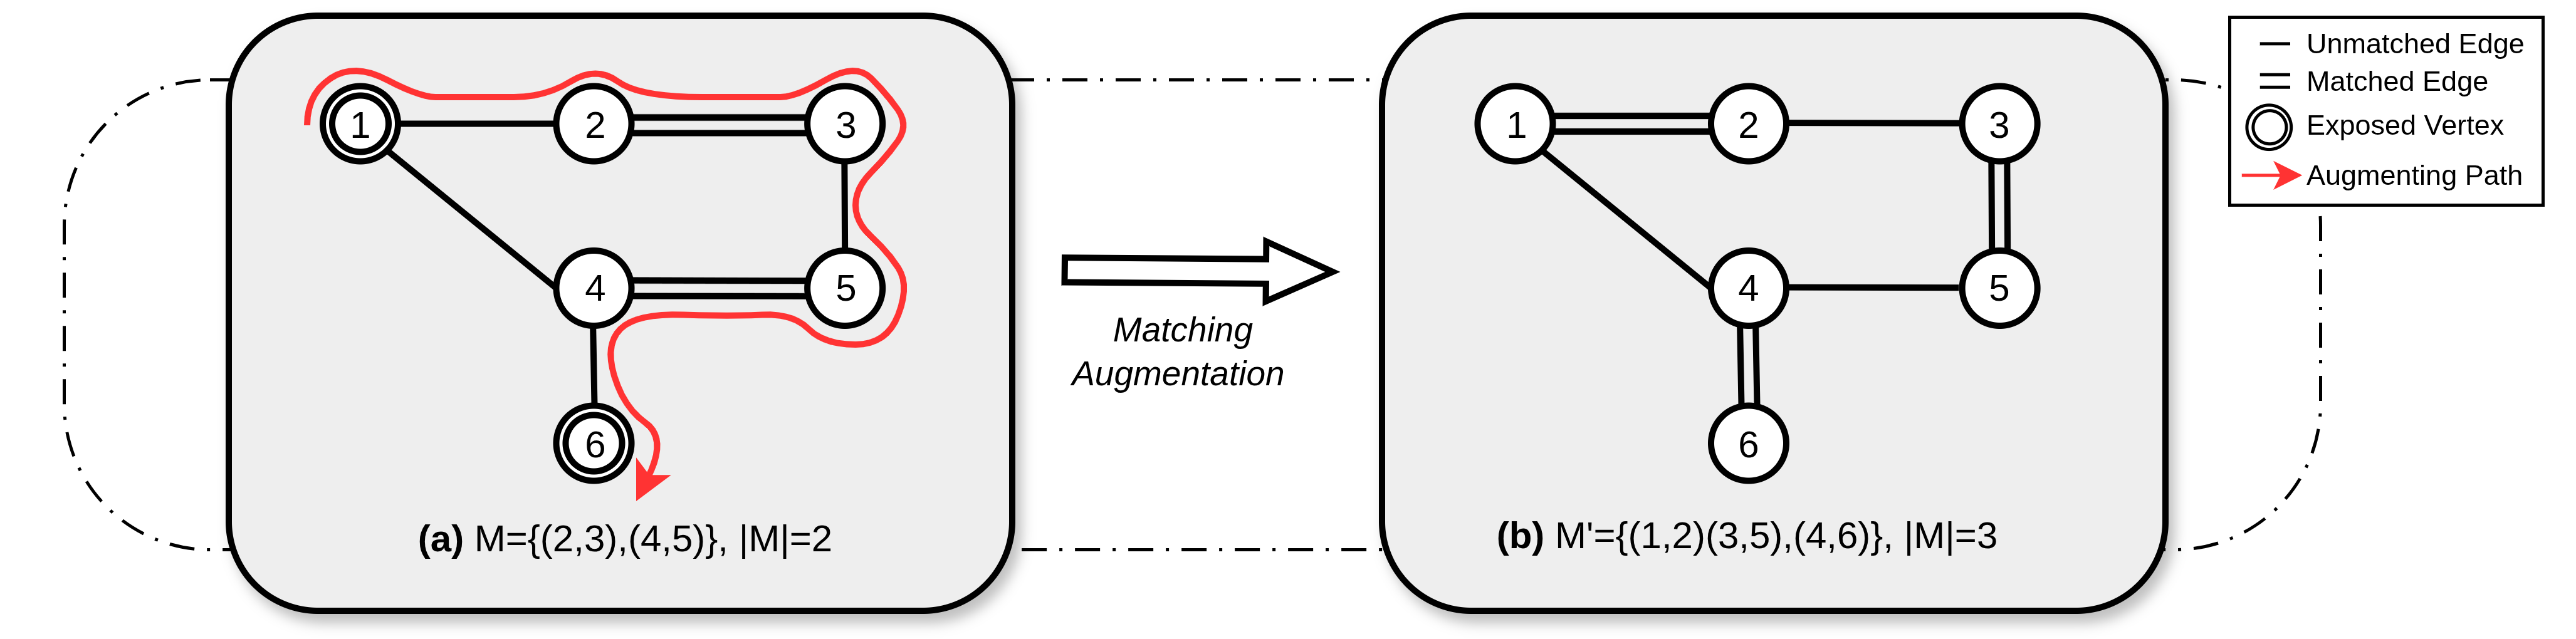
\includegraphics[width=0.80\columnwidth]{figures/diagrams/maximmum_matching.drawio.png}
	\captionsetup{skip=4pt}
	\caption{Maximum Matching and Augmenting Path}
	\label{Diagram:MaximumMatching}
\vspace{-4pt}
\end{figure}

Berge's theorem states that a matching is maximum iff no augmenting path exists.
Thus, Algorithm~\ref{Algo:MaximumMatchingAlgo} starts from the empty matching, repeatedly calls \textsc{Find-Augmenting-Path}, and augments along any returned path until the procedure returns empty.

\begin{algorithm}[!htbp]
  \small
  \captionsetup{font = footnotesize}
  \caption{The Maximum Matching Algorithm}
  \label{Algo:MaximumMatchingAlgo}
  \begin{algorithmic}[1]
    \Require A graph $G$
    \Ensure A maximum matching $M$

    \State $M \gets \emptyset$
    \Repeat
      \State $P \gets$ \Call{Find-Augmenting-Path}{$G$, $M$}
      \If{$P \neq \emptyset$}
        \State $M \gets (M \setminus P) \cup (P \setminus M)$ \Comment{augment $M$ along $P$}
      \EndIf
    \Until{$P = \emptyset$}
    \State \Return $M$

  \end{algorithmic}
\end{algorithm}

\subsection{Augmenting-Path Search via Alternating Trees}
Augmenting-path search uses an \emph{alternating forest}: alternating trees rooted at exposed vertices.
Each node is labeled even or odd by its depth from the root; exposed roots are even.
In Fig.~\ref{Diagram:AlternatingTrees}(a)--(b), exposed nodes~1 and~6 initialize two even-rooted trees.

\begin{figure}[!h]
	\centering
	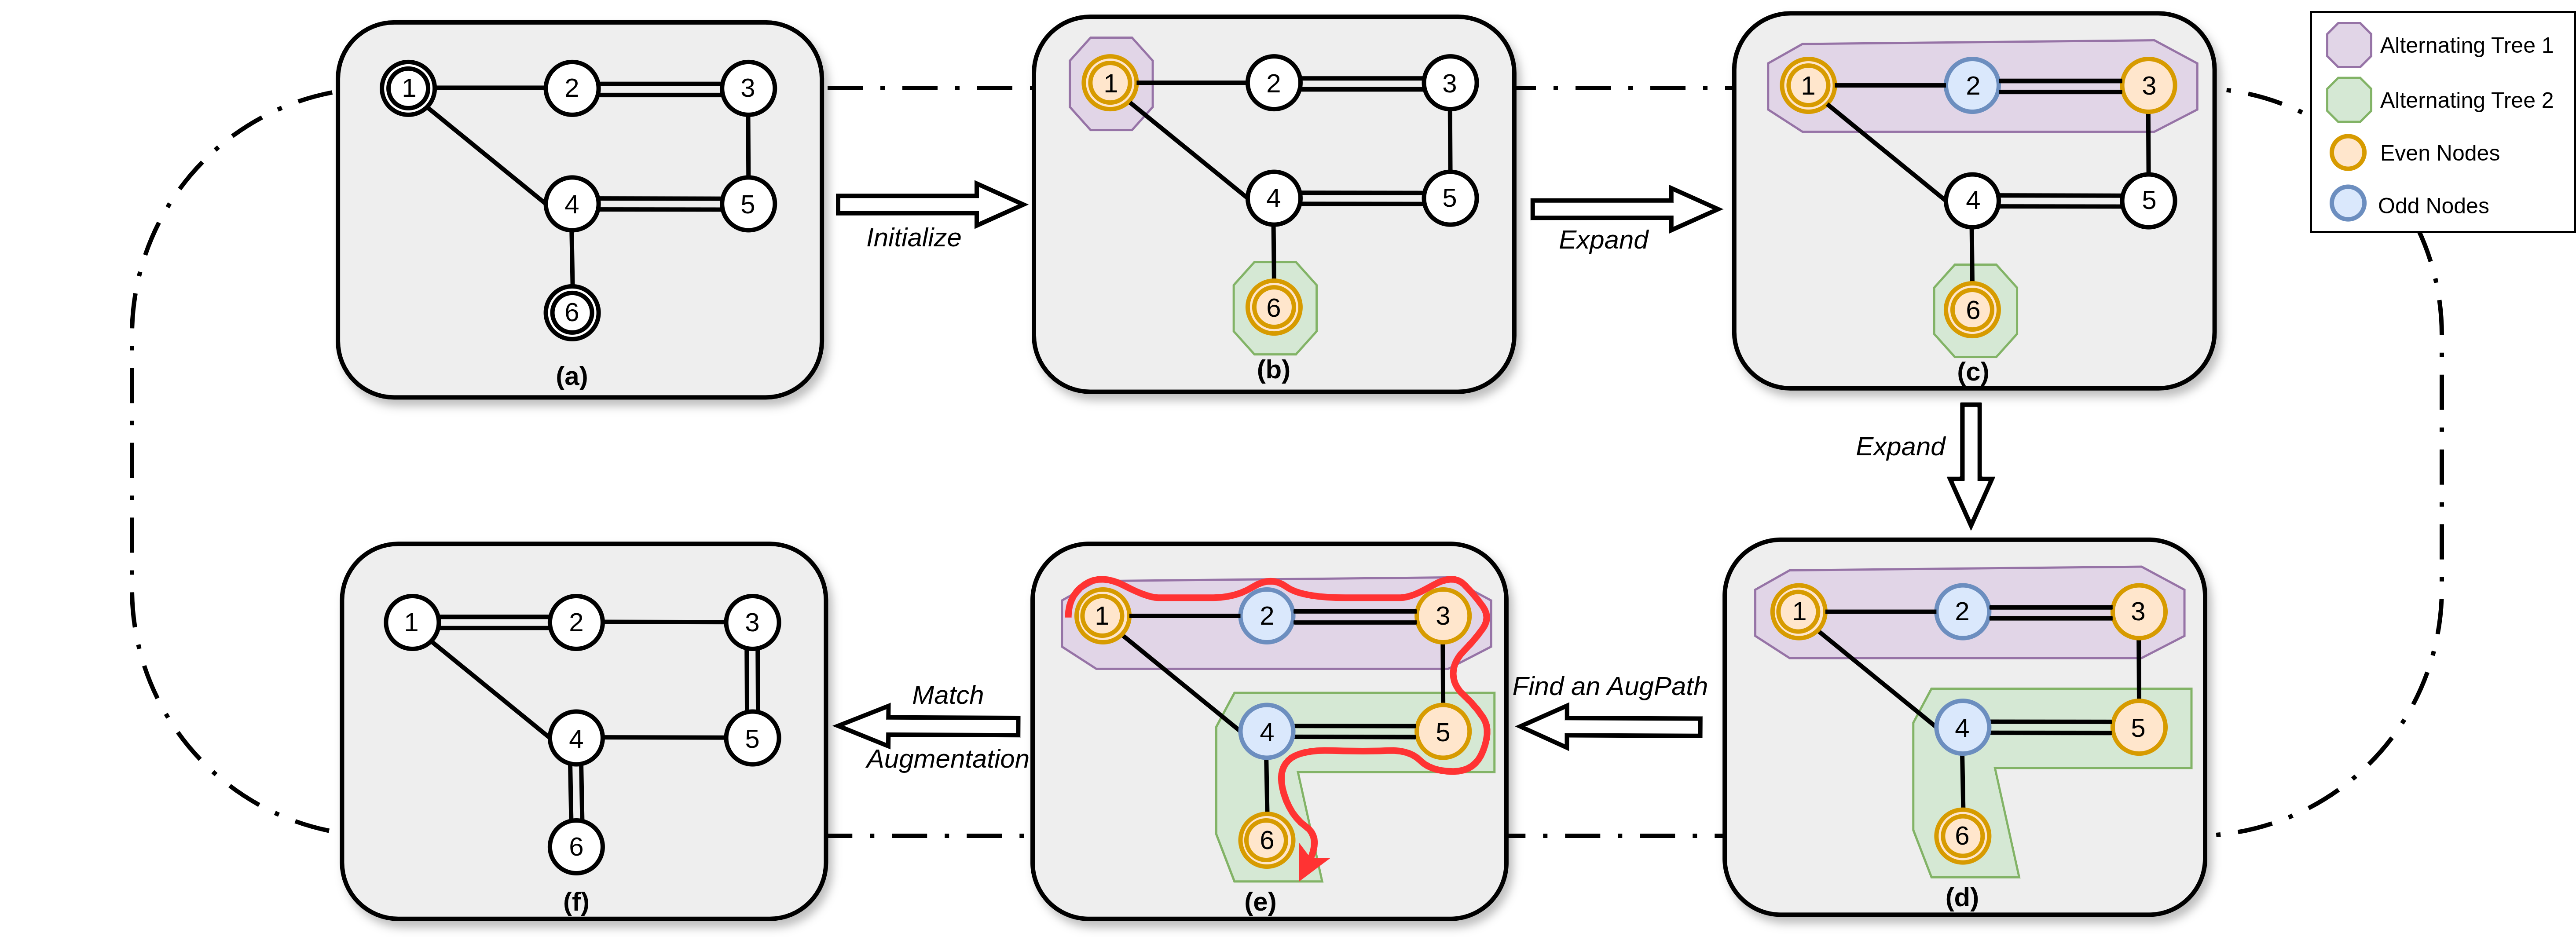
\includegraphics[width=1.0\columnwidth]{figures/diagrams/AlternatingTreesFewerSamples.drawio.png}
	\captionsetup{skip=4pt}
	\caption{The Augmenting-Path Search Procedure using Alternating Trees}
	\label{Diagram:AlternatingTrees}
\vspace{-4pt}
\end{figure}

% Expansion
Expansion starts only from even nodes and proceeds in two-edge steps: an unmatched edge to an odd node, then a matched edge to a new even node.
This preserves the invariant that every root-to-vertex path in an alternating tree has even length and starts with an unmatched edge.
In Fig.~\ref{Diagram:AlternatingTrees}(c), Tree~1 expands from node~1 to node~2 through an unmatched edge and then to node~3 through a matched edge, making nodes~2 and~3 odd and even, respectively.
Similarly, Fig.~\ref{Diagram:AlternatingTrees}(d) expands Tree~2 from node~6 through node~4 to node~5.
If an unmatched edge connects even vertices from different trees, their root-to-vertex paths plus this edge form an augmenting path.
In Fig.~\ref{Diagram:AlternatingTrees}(e), edge $(3,5)$ yields $1\!-\!2\!-\!3\!-\!4\!-\!5\!-\!6$, producing the larger matching in Fig.~\ref{Diagram:AlternatingTrees}(f).


% Key issue with this alternating-tree-expansion and augmenting-path detection mechanism => Blossom

\subsection{The Blossom Anomaly and Two Algorithmic Remedies}
% Although alternating trees work perfectly in bipartite graphs, their expansion may fail to discover an augmenting path in general graphs due to the presence of \emph{blossoms}.  
% A blossom is an odd-length alternating cycle that arises when two even-length root-to-vertex alternating paths in the \textbf{same} alternating tree are connected by an unmatched edge.
% And one node v of the cycle, the base of this blossom is such a node that there exists an alternating path of even length from this node to an exposed vertex.
% For example, in Fig.~\ref{Diagram:Blossoms}(a), the graph forms a blossom $1\!-\!2\!-\!3\!-\!5\!-\!4\!-1$ because the two even-length alternating paths $1\!-\!2\!-\!3$ and $1\!-\!4\!-\!5$ become connected by the unmatched edge $(3,5)$. And 1 is the base of this blossom because it has a even-length path of 0 from it to an exposed node, which is itself.

% Blossoms must be handled carefully because many of the alternating expansion patterns permitted by a blossom fail to expose augmenting paths that actually exist in the graph.  
% For instance, Fig.~\ref{Diagram:MaximumMatching} and ~\ref{Diagram:AlternatingTrees} shows that the graph indeed contains an augmenting path with respect to the given matching.  
% However, the blossom also permits an alternative expansion sequence that conforms to the alternating-tree expansion rules yet still fail to detect any augmenting path, since no unmatched edge ever connects two even vertices from distinct alternating trees.  

% % Two Blossom algorithms
% Blossom algorithms are augmenting-path search procedures with specific blossom handling subroutines.
% To our best knowledge, two sequential blossom algorithms are introduced: the classical recursive blossom algorithm and its modern non-recursive counterpart.
% Both of them handle blossoms by taking into consideration additional alternating-growth patterns necessary for augmenting path detection.
% % Recursive Blossom Algorithm
% The classical recursive algorithm handles a detected blossom by \emph{contracting} the entire odd cycle into a single super-vertex as shown in Fig.~\ref{Diagram:Blossoms}~(e) where the blossom is contracted into a single vertex 7.
% This super-vetex effectively represents all necessary alternating expansions through the contracted blossom.
% After that, in Fig.~\ref{Diagram:Blossoms}~(f) the augmenting-path search will continue on the contracted graph which results in an augmenting path (7,6)
% Then the algorithm performs a \emph{lifting} step in Fig~\ref{Diagram:Blossoms}~(g), expanding each contracted blossom with an even-length path from blossom base 1 to the connect node 4 in reverse order to recover a valid augmenting path in the original graph. 
% % Recursive-Free Blossom Algorithm
% For recursive-free blossom algorithm, upon detecting a blossom, the algorithm instead transform all odd nodes in the blossom into even nodes with a vliad even-length alternating path to the tree root. 
% This "evenification" of the blossom exposes new expansion opportunities, allowing formerly odd vertices to initiate further alternating-tree growth and augmenting-path detection
% In Fig~\ref{Diagram:Blossoms}~(i), nodes 2 and 4 are transformed into even nodes with even-length path 14532 and 12354. 
% After that, the augmenting path can be formed by connecting nodes 4 and 6 since both of them are even nodes.

Alternating-tree expansion is sufficient in bipartite graphs but can fail in general graphs because of \emph{blossoms}.
A blossom is an odd alternating cycle formed when an unmatched edge connects two even vertices in the same alternating tree; its \emph{base} has an even alternating path to an exposed root.
In Fig.~\ref{Diagram:Blossoms}(c), vertices $1\!-\!2\!-\!3\!-\!5\!-\!4\!-1$ form a blossom, and vertex~1 is the base.
Blossoms must be handled carefully because they permit alternating expansion patterns that obey the local tree rules but still fail to expose augmenting paths that exist in the graph.
Without special handling, the valid augmenting path shown in Figs.~\ref{Diagram:MaximumMatching} and~\ref{Diagram:AlternatingTrees} can be missed, as Fig.~\ref{Diagram:Blossoms}(a)--(c) illustrates.

\begin{figure}[!h]
	\centering
	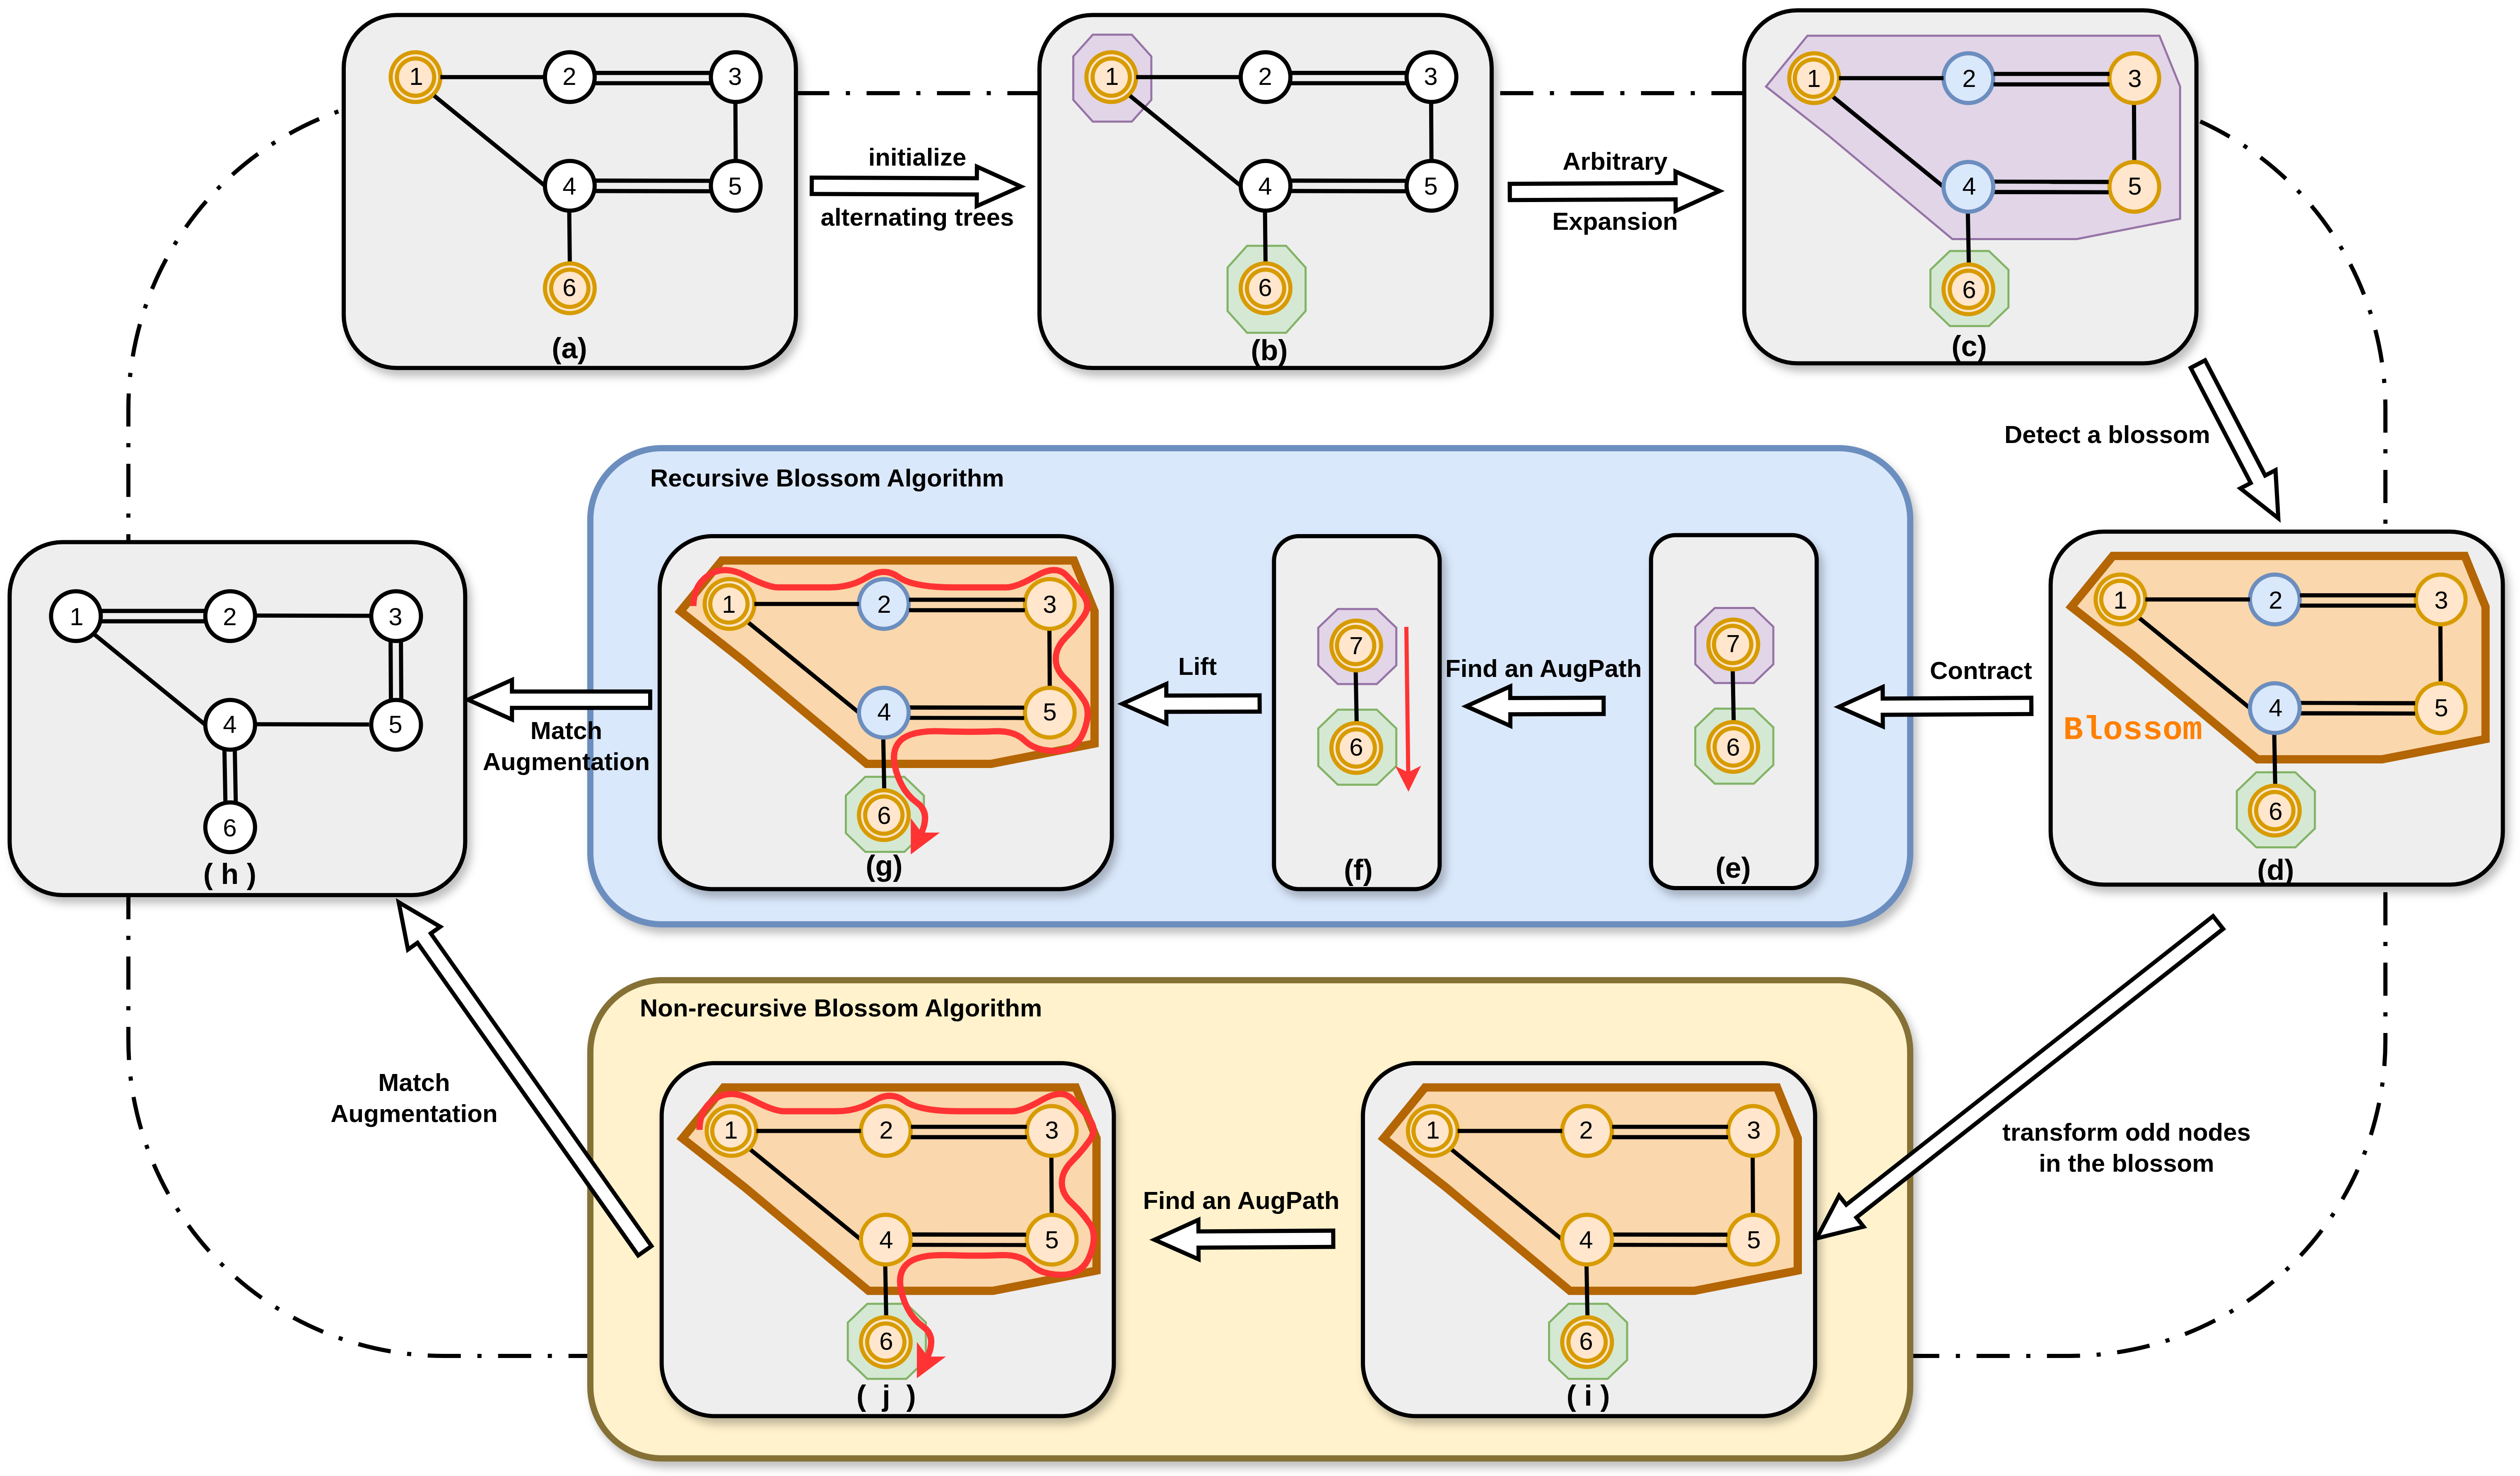
\includegraphics[width=0.95\columnwidth]{figures/diagrams/Blossoms.drawio.png}
	\captionsetup{skip=4pt}
	\caption{The formation of Blossoms and Two Blossom algorithms}
	\label{Diagram:Blossoms}
\vspace{-4pt}
\end{figure}

Two sequential remedies are commonly used: the classical recursive blossom algorithm and a recursion-free variant.
The recursive algorithm contracts a detected blossom into a super-vertex, continues the search on the contracted graph, and then \emph{lifts} the result back to the original graph.
In Fig.~\ref{Diagram:Blossoms}(d)--(h), the blossom becomes vertex~7; after an augmenting path is found, lifting selects the even path $4\!-\!5\!-\!3\!-\!2\!-\!1$ to reconstruct the original augmenting path.

The recursion-free algorithm avoids contraction by converting each odd blossom vertex into an even vertex with a valid even-length alternating path from the root.
This ``evenification'' lets these vertices continue tree expansion.
In Fig.~\ref{Diagram:Blossoms}(i), nodes~2 and~4 become even via paths $1\!-\!4\!-\!5\!-\!3\!-\!2$ and $1\!-\!2\!-\!3\!-\!5\!-\!4$; Fig.~\ref{Diagram:Blossoms}(j) then exposes an augmenting path.


\subsection{X-Blossom Parallel Framework}
The recursion-free algorithm is more amenable to parallelization because it avoids contraction and lifting, whose dynamic graph updates serialize computation.

% X-Blossom
X-Blossom is a parallel framework based on the recursion-free blossom algorithm for parallel augmenting-path search. As shown in Algorithm~\ref{Algo:XBlossom}, it maintains three auxiliary data structures:
\begin{itemize}[leftmargin=*]
    \item The checking set (frontier) $N$, containing the active even vertices whose incident edges are examined in the current iteration.
    \item The alternating forest $F$, consisting of alternating trees rooted at exposed vertices, each representing an independent search structure where even nodes are stored as the search progresses.
    \item The augmenting-path set $P$, which stores augmenting paths discovered during the search.
\end{itemize}

After initializing these structures from the exposed vertices, X-Blossom repeatedly executes three internally parallel procedures in sequence:  
(1) augmenting-path detection,  
(2) alternating-tree expansion, and  
(3) blossom handling.  
The iteration terminates either if an augmenting path is found or if no new even vertices can be generated, indicating that no further augmenting paths exist.
\phantomsection\label{para:xblossom-three-parallel-procedures}
\textcolor{blue}{At the implementation level, all three procedures partition the current checking set across worker threads, and each thread repeatedly scans the incident edges of its assigned frontier vertices.
Procedure~(1) detects augmenting paths by examining unmatched edges between even vertices from different alternating trees and recording vertex-disjoint candidates.
The expansion step then advances the search frontier: Procedure~(2) finds unmatched neighbors outside the current forest, follows their matched partners, and inserts the newly reached even vertices into the next frontier.
For blossom handling, Procedure~(3) inspects edges between even vertices in the same tree, identifies blossom structures, and converts eligible odd vertices into even vertices for subsequent expansion.}

% \vspace{-4pt}
\begin{algorithm}[!htbp]
  % \small
  \footnotesize
  \captionsetup{font = footnotesize}
  \caption{Parallel Augmenting-Path Search Procedure in X-Blossom}
  \label{Algo:XBlossom}
  \begin{algorithmic}[1]

  \Require Graph $G$ and matching $M$
  \Ensure A set of vertex-disjoint augmenting paths $P$, or empty if none exist

  \State $N \gets$ set of exposed vertices
  \State $F \gets$ set of trees rooted at exposed vertices
  \State $P \gets \emptyset$

  \While{$P = \emptyset \wedge N \neq \emptyset$}

      \State $P \gets$ \Call{Parallel-Augmenting-Path-Detection}{$G, M, N, F$}

      \State $N_{\text{next1}} \gets$ \Call{Parallel-Expand-Alternating-Trees}{$G, M, N, F$}

      \State $N_{\text{next2}} \gets$ \Call{Parallel-Blossom-Handling}{$G, M, N, F$}
      
      \State $N \gets N_{\text{next1}} \cup N_{\text{next2}}$

  \EndWhile
  
  \State \Return $P$

  \end{algorithmic}
\end{algorithm}
\vspace{-4pt}


\section{Accelerating X-Blossom on CPUs and GPUs}
We accelerate the original multi-core CPU implementation of X-Blossom in two steps. 
First, we propose X-Blossom-Pro, an optimized CPU realization that introduces alternating-tree reuse to remove duplicated computation across augmenting-path searches.
% and yields up to $3.26\times$ speedup over the original CPU implementation. 
Second, we develop X-Blossom++, the first GPU implementation of the blossom algorithm.
X-Blossom++ maps X-Blossom-Pro's dynamic data structures to GPUs and uses fine-grained edge-level GPU load balancing.
% As a result, X-Blossom++ achieves up to $39.09\times$ speedup over X-Blossom-Pro.

\subsection{X-Blossom-Pro: An Enhanced Implementation of X-Blossom for Multi-Core CPUs}
\label{subsec:reuse}
Maximum matching invokes augmenting-path search repeatedly.
After a matching augmentation between two calls, the previously exposed roots of alternating trees that participate in a discovered augmenting path become matched.
These newly matched vertices can no longer serve as valid exposed roots, so their associated trees must be cleared.
% Connecting Sentence
Algo.~\ref{Algo:XBlossom} handles this root-status change by clearing all alternating trees before each subsequent call, but this is overly conservative.
Trees not involved in any discovered augmenting path remain rooted at exposed vertices, structurally intact, and reusable across iterations.
% Since their roots remain exposed after augmentation, 

% \vspace{-4pt}
\begin{algorithm}[!htbp]
  % \small
  \footnotesize
  \captionsetup{font = footnotesize}
  \caption{Parallel Augmenting-Path Search Procedure with Reusable Alternating Trees in X-Blossom-Pro}
  \label{Algo:Reuse}
  \begin{algorithmic}[1]

  \Require Graph $G$ and matching $M$
  \Ensure A set of vertex-disjoint augmenting paths $P$, or empty if none exist

  \State $S_{\text{exposed}} \gets $ set of exposed vertices
  \State $S_{\text{reuse}} \gets $ non-root even nodes in surviving alternating trees
  \State $S_{\text{reset}} \gets $ non-root even nodes in cleared alternating trees
  \State $N \gets  S_{\text{exposed}} \cup S_{\text{reuse}} $
  \State $F \gets F_\text{old} \cup S_{\text{exposed}} - S_{\text{reset}}$
 
  \State $P \gets \emptyset$
  
  \While{$P = \emptyset \wedge N \neq \emptyset$}

      \State $P \gets$ \Call{Parallel-Augmenting-Path-Detection}{$G, M, N, F$}
      % \If{$P_{\text{total}} \neq \emptyset$}
      %     \State \Return $P_{\text{total}}$
      % \EndIf

      \State $N_{\text{next1}} \gets$ \Call{Parallel-Expand-Alternating-Trees}{$G, M, N, F$}

      \State $N_{\text{next2}} \gets$ \Call{Parallel-Blossom-Handling}{$G, M, N, F$}
      
      \State $N \gets N_{\text{next1}} \cup N_{\text{next2}}$

  \EndWhile
  
  \State \Return $P$

  \end{algorithmic}
\end{algorithm}

Motivated by alternating-tree reuse in bipartite graphs~\cite{akathoott2025bidirectional}, we extend reuse to general graphs with blossoms.
Algo.~\ref{Algo:Reuse} partitions even vertices after each augmentation into exposed vertices, reusable non-root even vertices in surviving trees, and non-root even vertices in trees that must be reset (lines 1--3).
The new checking set combines exposed and reusable even vertices (line 4), so all retained vertices re-enter the three parallel subroutines and preserve the correctness guarantee of~\cite{fan2025x}.
The alternating forest then keeps only surviving trees and removes those whose roots became matched (line 5).
The remaining search follows Algo.~\ref{Algo:XBlossom} while avoiding regrowth of structurally valid trees.


\subsection{X-Blossom++: The First GPU-Accelerated Blossom Algorithm Implementation}
\label{subsec:xb++}
% In this section, we present the first GPU implementation of the blossom algorithm, termed X-Blossom++. Building upon the optimizations introduced in X-Blossom-Pro, X-Blossom++ maps the algorithm’s dynamic data structures onto GPUs and further addresses the inherent irregular and imbalanced parallelism of X-Blossom.

% This is an easy one, but still worth mentioning as one necessary step. 
\subsubsection{Dynamic Data Structure Representations on GPUs}
\label{subsub:repOnGPU}
% Introduction to GPU representation of path tables
X-Blossom uses highly dynamic structures, including the path table and checking set, with frequent insertions and deletions.
On CPUs, standard resizable containers handle allocation, growth, and reclamation efficiently.
On GPUs, CUDA allocation APIs such as \texttt{cudaMalloc} and \texttt{cudaFree} are costly~\cite{guo2024gmlake}, and higher-level containers such as Thrust inherit this cost under frequent updates.
Thus, X-Blossom++ uses explicit memory-management strategies for these dynamic structures.

\begin{figure}[!h]
	\centering
	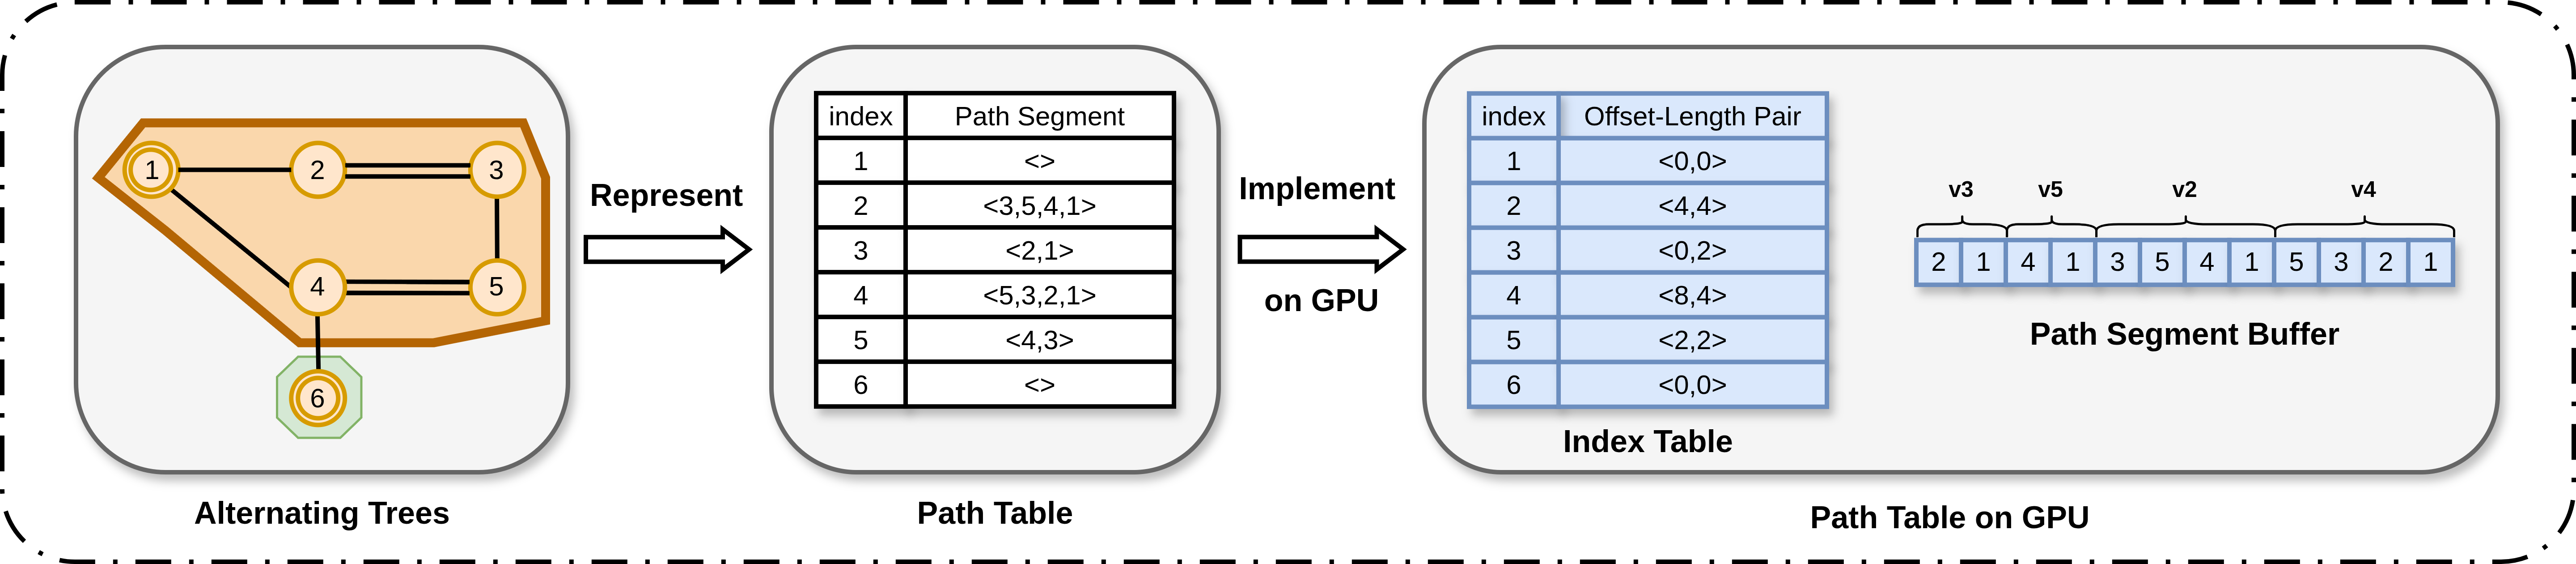
\includegraphics[width=1.0\columnwidth]{figures/diagrams/PathTableGPU.drawio.png}
	\captionsetup{skip=4pt}
	\caption{Alternating Trees, Path Table, and Path Table Implementation on GPUs}
	\label{Diagram:PathTable}
\vspace{-4pt}
\end{figure}

% Path Table on GPUs has an additional index table to be functional and efficient
A \emph{path table} compactly represents the alternating forest by mapping each even vertex to a \emph{path segment}.
As shown in Fig.~\ref{Diagram:PathTable}, roots such as 1 and 6 store empty segments.
Vertices added by expansion store the segment back to the previous even vertex: vertex~3 stores $\langle 2,1\rangle$, and vertex~5 stores $\langle 4,3\rangle$.
When blossom handling converts an odd vertex into an even vertex, it stores the segment through the blossom base; vertex~2 traces to base~1 through $3 \rightarrow 5 \rightarrow 4 \rightarrow 1$ and stores $\langle 3,5,4,1\rangle$.

On the GPU, the path table has an \emph{index table}, which maps each even vertex to an offset--length pair, and a contiguous \emph{path segment buffer}.
For example, vertex~2 stores $(4,4)$, meaning its four-element segment starts at offset~4.
% atomic counter
An atomic counter tracks the next available buffer offset.
Inserting a segment atomically reserves a contiguous region, writes the segment there, and records the offset--length pair in the index table.
% checking set
Similarly, the \emph{checking set} uses an array for newly added even vertices and an atomic counter for insertion positions.

\subsubsection{Two Workload Balancing Strategies}
\label{subsub:load-balancing}
Like other traversal algorithms, X-Blossom repeatedly processes incident edges of vertices in the current frontier across its three parallel phases.
Sparse graphs are stored in CSR format, where \emph{column indices} store neighbor vertices contiguously and \emph{row offsets} give each vertex's neighbor-list start.
Thus, processing frontier edges is equivalent to scanning the corresponding column-indices segments.
In Fig.~\ref{Diagram:Load-Balancing}, vertices 1--4 form the frontier; vertex~4 reads row-offset value 6 and scans $\langle v_3, v_5, v_6, v_7\rangle$.

% Two types of load-balancing strategy.
\begin{figure}[!h]
	\centering
	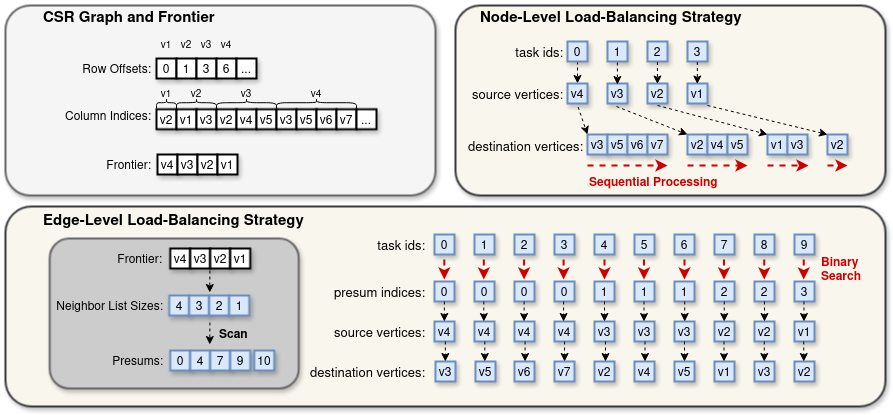
\includegraphics[width=1.0\columnwidth]{figures/diagrams/LoadBalanceStrategy.drawio.png}
	\captionsetup{skip=4pt}
	\caption{Two Load-Balancing Strategies}
	\label{Diagram:Load-Balancing}
\vspace{-4pt}
\end{figure}

% coarse-grained strategy
% In the coarse-grained, vertex-level strategy, each frontier vertex is treated as the indivisible unit of parallel work.
% Once an active frontier vertex is assigned to a thread, the thread loads the vertex’s neighbor-list offset and then serially scans and processes all of its incident edges.
Efficient frontier processing depends on workload distribution.
We consider two granularities: coarse-grained vertex-level (node-level) scheduling and fine-grained edge-level scheduling.
The vertex-level strategy creates one task per frontier vertex.
Each task reads \texttt{Row Offsets} and scans the corresponding \texttt{Column Indices} segment.
As Fig.~\ref{Diagram:Load-Balancing} shows, vertices 0--3 map to tasks 0--3, so different neighbor lists run in parallel but each list is scanned serially.
% Although the vertex-level strategy exposes parallelism across frontier vertices with minimal scheduling overhead, it underutilizes the available parallelism because all edges incident to a frontier vertex are independent and could, in principle, be processed concurrently. 
This design has low scheduling overhead but can underutilize parallelism because incident edges are independent.
It is also sensitive to skewed degree distributions: a high-degree frontier vertex can make its assigned thread process substantially more edges than other threads.
In the example, vertex $v_3$ has three neighbors while $v_1$ has one, so the thread processing $v_1$ can become idle while the thread processing $v_3$ remains busy.
% Moreover, in the context of X-Blossom, the imbalance is further amplified because a thread may also perform expensive blossom-related operations, such as detecting blossom bases and materializing blossoms, making the per-vertex workload even more irregular.
In X-Blossom, imbalance can be amplified when some vertices trigger costly blossom operations, such as tracing two endpoint-to-root paths to find the base and materializing the odd cycle.

% fine-grained strategy
The edge-level strategy instead creates one task per frontier edge.
It first builds an array of neighbor-list sizes and performs a prefix-sum scan, compacting sparse, skewed per-vertex work into dense per-edge tasks.
The resulting prefix-sum array records the cumulative number of incident edges contributed by frontier vertices, and its final entry gives the total number of frontier edges to process.
In Fig.~\ref{Diagram:Load-Balancing}, the frontier contributes ten edges, so ten tasks are generated.
Each task uses its ID to locate the corresponding frontier vertex by binary-searching the prefix-sum array.
For example, task IDs 4--6 map to prefix index~1, vertex $v_3$, and offsets 0--2, corresponding to neighbors $v_2$, $v_4$, and $v_5$.
By assigning one task per frontier edge, this strategy processes all incident edges in parallel rather than serially scanning each neighbor list.
However, compaction adds per-edge lookup overhead, which can be costly on platforms where binary searches and indirect indexing are expensive.
We evaluate both strategies in \S~\ref{subsubsec:exp_load_balancing}; edge-level load balancing is superior for X-Blossom++, whereas node-level scheduling is more effective for X-Blossom-Pro.

\begin{comment}
\subsection{On-the-fly Blossoeem-Base Identification}
The blossom-base identification is a prerequisite step before constructing a blossom as the concatenation of the paths from the base to each endpoint. 
This procedure takes as input an alternating tree, its root, and two even endpoints that form a blossom, and returns the blossom base. 
For example, given the alternating tree in Fig.~\ref{Diagram:OnTheFly} with root \(1\) and even endpoints \(9\) and \(11\), the goal of blossom-base identification is to return vertex \(5\) as the blossom base, which will later be used to construct the blossom cycle \(5 \to 6 \to 7 \to 8 \to 9 \to 11 \to 10 \to 5\).
% Path Table
During this process, each alternating tree is represented by a \emph{path table}, in which every even vertex stores the path segment from its preceding even vertex to itself (the right-hand table in Fig.~\ref{Diagram:OnTheFly}). For instance, even vertex \(9\) stores the segment \(\langle 9,8,7\rangle\). The root vertex \(1\) stores an empty path, since it has no preceding even vertex, and vertices \(2,4,6,8,10\) are odd, so they do not store any path segments in the table.


\begin{figure}[!h]
	\centering
	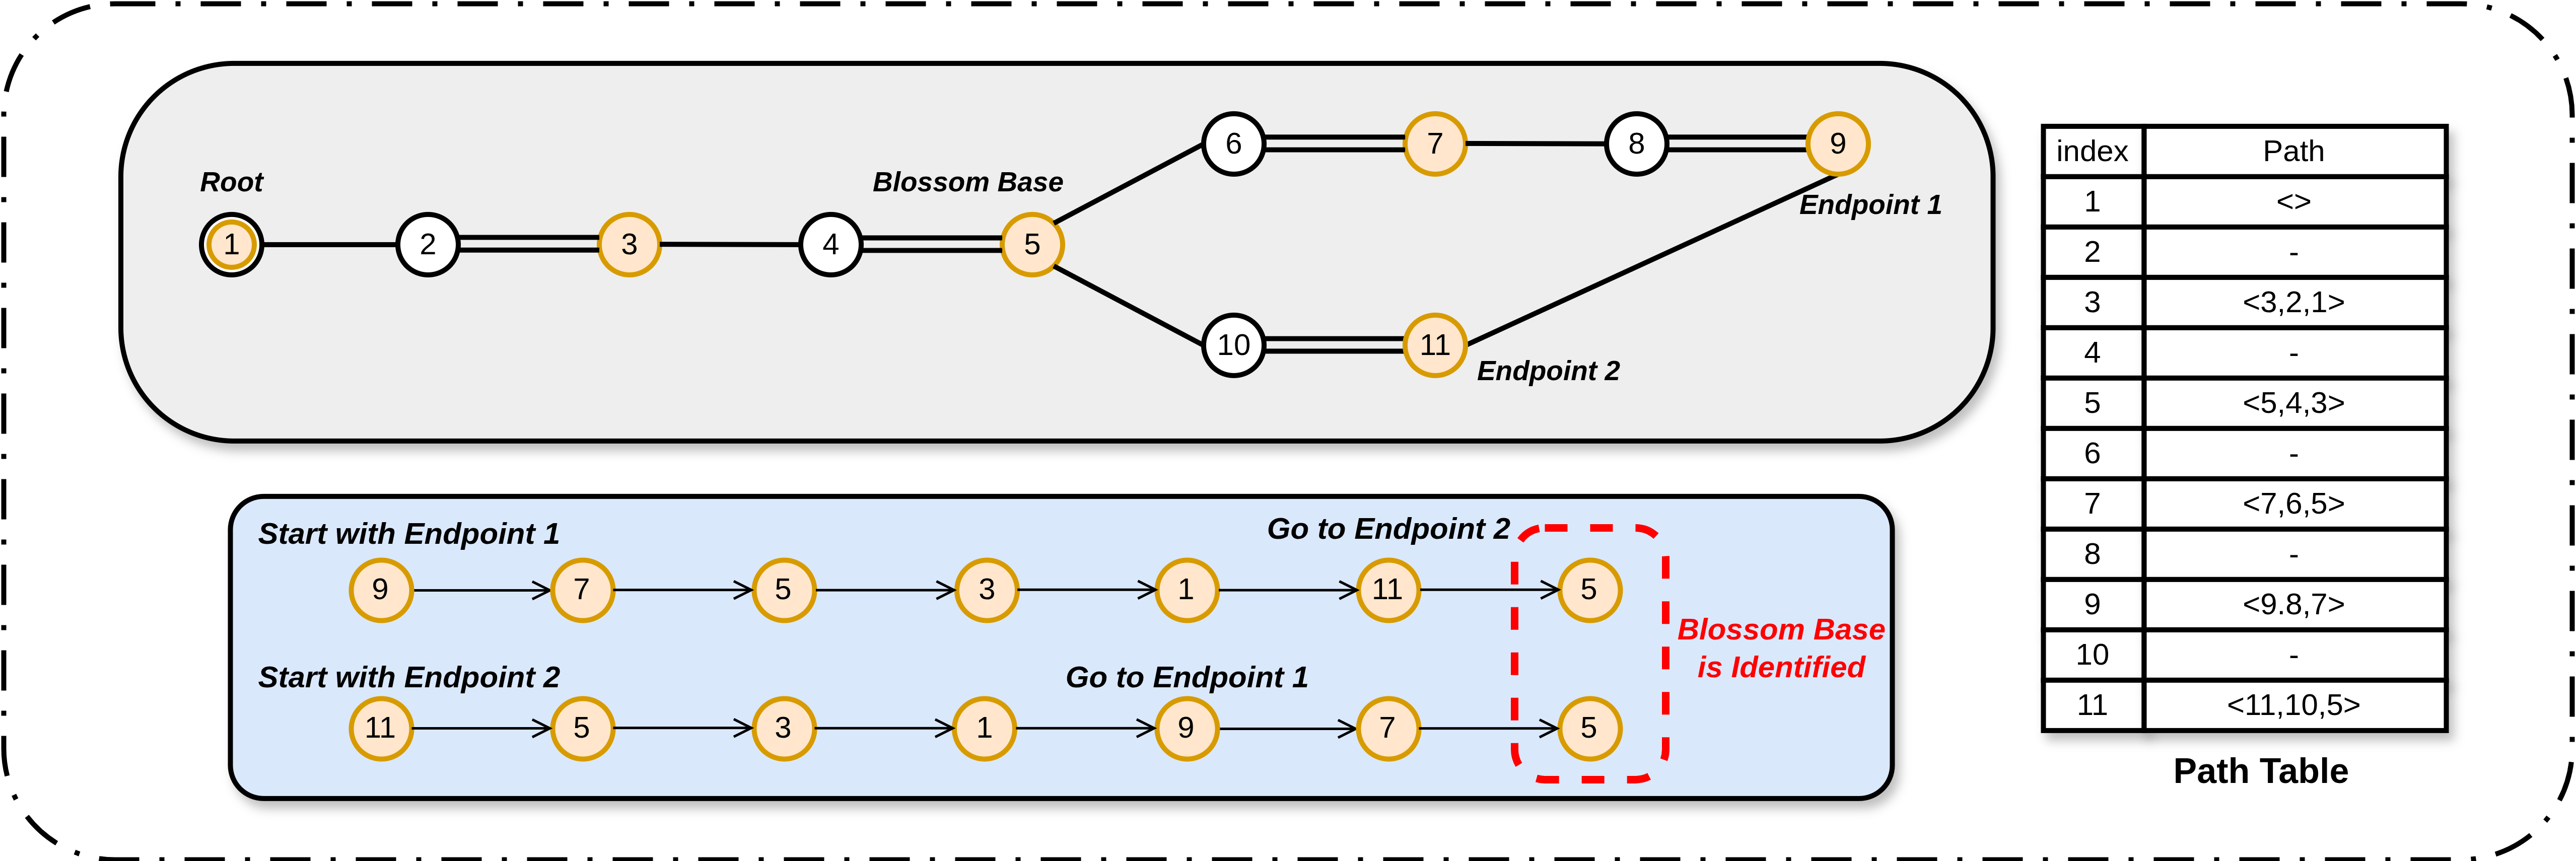
\includegraphics[width=1.0\columnwidth]{figures/diagrams/OnTheFlyIdenOnly.drawio.png}
	\captionsetup{skip=4pt}
	\caption{The On-The-Fly Blossom-Base Identification}
	\label{Diagram:OnTheFly}
\vspace{-4pt}
\end{figure}

The current blossom-base identification strategy reconstructs the full paths from each endpoint to the root and then identifies the base by locating the first divergence in these two paths. Concretely, starting from Endpoint~1 and Endpoint~2, it reconstructs the sequences
\(9 \to 8 \to 7 \to 6 \to 5 \to 4 \to 3 \to 2 \to 1\) and
\(11 \to 10 \to 5 \to 4 \to 3 \to 2 \to 1\),
stores them in temporary buffers, and scans the buffers from the root toward the leaves until the paths split at the outgoing edges \(5 \to 6\) and \(5 \to 10\). 
The last common vertex, \(5\), is then identified as the blossom base. 
This procedure is wasteful because it stores two full endpoint-to-root paths. In particular, the shared suffix from the base to the root,
\(5 \to 4 \to 3 \to 2 \to 1\), is materialized and scanned twice, once for each endpoint, even though this segment is not needed for constructing the blossom itself.

To avoid full endpoint-to-root path materialization, we adopt an \emph{on-the-fly} blossom-base identification scheme. 
We start two walks from the two endpoints simultaneously.
Each walk repeatedly moves from its current even vertex to its preceding even vertex until the two walks reach the same vertex. 
Whenever a walk reaches the root, it jumps to the opposite endpoint and continues. 
As illustrated in the lower panel of Fig.~\ref{Diagram:OnTheFly}, one walk follows \(9 \to 7 \to 5 \to 3 \to 1\) and then jumps to \(11 \to 5\), while the other walk follows \(11 \to 5 \to 3 \to 1\) and then jumps to \(9 \to 7 \to 5\). 
At the same iteration, both walks arrive at vertex \(5\), which is identified as the blossom base. 
% This base is subsequently used to materialize the blossom by combining the segments from the base to each endpoint.
    
\end{comment}


\section{Intensive Experiments for Performance Insights}
\label{sec:intensive-experiments}

\subsection{Evaluation Platform Settings}
\subsubsection{Experimental Environment.}
\label{subsubsec:eval-exp-env}
\textcolor{blue}{
All experiments were conducted on two server-class Amazon Web Services (AWS) instances running Ubuntu 24.04.4 LTS. 
The \phantomsection\label{para:exp-setup-cpu}central processing unit (CPU)-based baselines were evaluated on an m7i.metal-24xl instance equipped with an Intel Xeon Platinum 8488C CPU with 48 physical cores, 96 hardware threads, 105 MB L3 cache, and 405 GB RAM.
In our experiments, CPU implementations use at most 48 software threads, assigning at most one worker thread to each physical core and avoiding multithreading.
The \phantomsection\label{para:exp-setup-gpu}graphics processing unit (GPU)-based baselines were evaluated on a g7e.8xlarge instance equipped with an NVIDIA RTX PRO 6000 Blackwell Server Edition GPU with 96 GB GPU memory, compute capability 12.0, NVIDIA driver 595.71.05, and CUDA 13.2.
We used two separate instances because the CPU baselines require a bare-metal instance to expose memory-system information, whereas AWS GPU instances do not provide this capability. 
All code was compiled with -O3 optimizations. The software stack included g++ 13.3.0, CMake 4.3.1, and CUDA Toolkit 13.2.
Parallel execution for our implementations follows their target architectures: X-Blossom-Pro (XB-Pro) relies on C++ \texttt{std::thread} backed by pthreads, while X-Blossom++ (XB++) launches CUDA kernels.
}

\subsubsection{Datasets.}
The ten real-world graph datasets used to evaluate our baselines are summarized in Table~\ref{tab:graph-metrics}.
% basic size
Drawn from the SNAP collection \cite{SNAP_Dataset}, these datasets span diverse application domains and exhibit substantial variation in the numbers of nodes and edges.
\phantomsection\label{para:real-world-sparse-datasets}
\textcolor{blue}{In this paper, we focus on real-world sparse graph datasets to align the evaluation with the graph structures commonly observed in large-scale network-analysis workloads.
% , where irregular degree distributions, sparse connectivity, and frontier-dependent parallelism strongly affect CPU and GPU behavior.
}
% other properties
In addition to the number of nodes and edges, we report several structural properties to better characterize each graph, including the maximum degree (Max~Deg), average degree (Avg~Deg), the total number of blossoms processed by the X-Blossom framework (Blossoms), and the average number of blossoms per node (Avg~Blossoms), as shown in Table~\ref{tab:graph-metrics}.
% graph metrics
Max~Deg represents the largest number of edges incident to any single node in the graph. 
Avg~Deg is computed as the ratio of the total number of edges to the number of nodes, providing a normalized measure of workload that enables fair comparisons across graphs of different sizes.
% Blossoms corresponds to the total count of blossoms processed by the X-Blossom framework; reported values are averaged over ten independent runs of X-Blossom-Pro. 
Finally, Avg~Blossoms is computed as total blossoms divided by the number of nodes.

\begin{table*}[h]
 \footnotesize
 \centering
 \setlength{\tabcolsep}{9pt}
 \renewcommand{\arraystretch}{1.0}
 \begin{tabular*}{\textwidth}{@{\extracolsep{\fill}}c|rrrcc}
 \toprule
 Dataset &
 $|V|$ &
 $|E|$ &
 Max Deg. &
 Avg Deg. &
 Avg~Blossoms \\
 \midrule
 GPlus & 107,614 & 12,238,285 & 20127 & 114 & 80.1 {\tiny $\pm$ 5.77} \\
 Twitch & 168,114 & 6,797,557 & 35279 & 40.4 & 8.43 {\tiny $\pm$ 2.25} \\
 Amazon & 334,863 & 925,872 & 549 & 2.76 & 7.85 {\tiny $\pm$ 0.096} \\
 HiggsNets & 456,626 & 12,508,409 & 51386 & 27.4 & 0.714 {\tiny $\pm$ 0.236} \\
 Youtube & 1,134,890 & 2,987,624 & 28754 & 2.63 & 0.048 {\tiny $\pm$ 0.001105} \\
 Hyperlink & 1,791,489 & 25,444,206 & 238342 & 14.2 & 3.81 {\tiny $\pm$ 0.143} \\
 Wikipedia & 2,394,385 & 4,659,565 & 100029 & 1.95 & 0.000523 {\tiny $\pm$ 0.000015} \\
 StackOverflow & 2,601,977 & 28,183,518 & 44065 & 10.8 & 0.000570 {\tiny $\pm$ 0.000016} \\
 Patent & 3,774,768 & 16,518,947 & 793 & 4.38 & 1.00 {\tiny $\pm$ 0.229} \\
 LiveJournal & 4,847,571 & 42,851,237 & 20333 & 8.84 & 5.25 {\tiny $\pm$ 0.116} \\
 \bottomrule
 \end{tabular*}
 \captionsetup{skip=4pt}
 \caption{
 Graph structural metrics and blossom statistics for the evaluated datasets.
 Avg~Blossoms entries are reported as mean $\pm$ 95\% confidence interval over 50 rounds.
 }
 \label{tab:graph-metrics}
\vspace{-4pt}
\end{table*}


\subsection{Performance Evaluation and Analysis of XB-Pro and XB++}
\subsubsection{Effectiveness of Reusing Alternating Trees}
\label{subsub:exp_reuse}
Reusing alternating trees is an algorithmic optimization for the X-Blossom framework that is independent of hardware platforms and can be applied to both CPU and GPU implementations.
We evaluate the effectiveness of reusing alternating trees in both XB-Pro (CPU) and XB++ (GPU) by comparing implementations with and without this optimization across ten real-world graph datasets; the results are reported in Table~\ref{tab:reuse}.
On the CPU, the baseline X-Blossom (XB) does not support alternating-tree reuse, whereas XB-Pro enables this optimization.
On the GPU, we compare XB++ with X-Blossom-GPU (XB-GPU), a naive GPU implementation of the original X-Blossom algorithm.
Specifically, XB-GPU uses the dynamic data structures described in \S~\ref{subsub:repOnGPU} and the edge-level load-balancing strategy presented in \S~\ref{subsub:load-balancing}, but does not incorporate the alternating-tree reuse technique introduced in \S~\ref{subsec:reuse}.
As shown in Table~\ref{tab:reuse}, speedups are computed as the runtime without alternating-tree reuse (XB or XB-GPU) divided by the runtime with reuse (XB-Pro or XB++).
Across all real-world graphs, alternating-tree reuse consistently improves performance on both CPU and GPU.
On the CPU, XB-Pro outperforms XB on all datasets, achieving speedups ranging from 1.20$\times$ to 3.26$\times$.
On the GPU, the performance gains from this technique are more pronounced, with speedups ranging from 1.24$\times$ to 5.68$\times$.
\textcolor{blue}{To explain this variability, Table~\ref{tab:reuse} reports ReuseRatio, defined as the percentage of alternating-tree nodes preserved by the reuse mechanism rather than reset. 
A higher ReuseRatio means that more previously constructed search state can be carried across iterations, reducing repeated tree reconstruction. 
This metric tracks the observed speedups: Amazon, Patent, and LiveJournal have the three highest ReuseRatio values on both CPU and GPU and also achieve the largest reuse speedups. 
In contrast, Wikipedia has the lowest ReuseRatio on both platforms and correspondingly shows the smallest benefit from reuse.}

\begin{table*}[h]
 \scriptsize
 % \small
 \centering
 \setlength{\tabcolsep}{3pt}
 \renewcommand{\arraystretch}{1.0}
 \resizebox{\textwidth}{!}{%
 \begin{tabular}{l|cccc|cccc}
 \toprule
  & \multicolumn{4}{c|}{\textbf{CPU}}
  & \multicolumn{4}{c}{\textbf{GPU}} \\
 \cmidrule(lr){2-5} \cmidrule(lr){6-9}
 Dataset &
 XB &
 XB-Pro &
 Speedup &
 ReuseRatio (\%) &
 XB-GPU &
 XB++ &
 Speedup &
 ReuseRatio (\%) \\
 \midrule
 Amazon & 1.49 {\tiny $\pm$ 0.0432} & 0.458 {\tiny $\pm$ 0.0105} & 3.26$\times$ & 42.4 {\tiny $\pm$ 0.3} & 0.444 {\tiny $\pm$ 0.0142} & 0.0781 {\tiny $\pm$ 0.0041} & 5.68$\times$ & 39.6 {\tiny $\pm$ 0.2} \\
 Patent & 8.23 {\tiny $\pm$ 0.366} & 5.05 {\tiny $\pm$ 0.184} & 1.63$\times$ & 32.1 {\tiny $\pm$ 0.1} & 0.567 {\tiny $\pm$ 0.0145} & 0.122 {\tiny $\pm$ 0.0045} & 4.64$\times$ & 31.9 {\tiny $\pm$ 0.08} \\
 LiveJournal & 16.8 {\tiny $\pm$ 0.554} & 8.08 {\tiny $\pm$ 0.320} & 2.08$\times$ & 31.0 {\tiny $\pm$ 0.1} & 0.916 {\tiny $\pm$ 0.0372} & 0.237 {\tiny $\pm$ 0.0031} & 3.86$\times$ & 27.3 {\tiny $\pm$ 0.1} \\
 StackOverflow & 1.57 {\tiny $\pm$ 0.0792} & 1.22 {\tiny $\pm$ 0.0392} & 1.28$\times$ & 20.2 {\tiny $\pm$ 0.6} & 0.0460 {\tiny $\pm$ 0.0018} & 0.0284 {\tiny $\pm$ 0.0009} & 1.62$\times$ & 19.3 {\tiny $\pm$ 0.3} \\
 GPlus & 1.54 {\tiny $\pm$ 0.0461} & 1.21 {\tiny $\pm$ 0.0763} & 1.27$\times$ & 18.4 {\tiny $\pm$ 0.06} & 0.389 {\tiny $\pm$ 0.0086} & 0.177 {\tiny $\pm$ 0.0034} & 2.20$\times$ & 18.8 {\tiny $\pm$ 0.06} \\
 Hyperlink & 4.69 {\tiny $\pm$ 0.148} & 3.42 {\tiny $\pm$ 0.124} & 1.37$\times$ & 18.3 {\tiny $\pm$ 0.06} & 0.548 {\tiny $\pm$ 0.0099} & 0.171 {\tiny $\pm$ 0.0024} & 3.21$\times$ & 17.8 {\tiny $\pm$ 0.04} \\
 Youtube & 0.442 {\tiny $\pm$ 0.0277} & 0.345 {\tiny $\pm$ 0.0167} & 1.28$\times$ & 17.3 {\tiny $\pm$ 0.5} & 0.0276 {\tiny $\pm$ 0.0010} & 0.0161 {\tiny $\pm$ 0.0005} & 1.71$\times$ & 16.4 {\tiny $\pm$ 0.3} \\
 HiggsNets & 0.902 {\tiny $\pm$ 0.0203} & 0.572 {\tiny $\pm$ 0.0154} & 1.58$\times$ & 14.3 {\tiny $\pm$ 0.06} & 0.239 {\tiny $\pm$ 0.0075} & 0.0755 {\tiny $\pm$ 0.0015} & 3.17$\times$ & 14.3 {\tiny $\pm$ 0.09} \\
 Twitch & 0.503 {\tiny $\pm$ 0.0155} & 0.403 {\tiny $\pm$ 0.0380} & 1.25$\times$ & 6.2 {\tiny $\pm$ 0.04} & 0.209 {\tiny $\pm$ 0.0052} & 0.0909 {\tiny $\pm$ 0.0018} & 2.30$\times$ & 6.3 {\tiny $\pm$ 0.03} \\
 Wikipedia & 0.557 {\tiny $\pm$ 0.0375} & 0.462 {\tiny $\pm$ 0.0285} & 1.20$\times$ & 1.6 {\tiny $\pm$ 0.03} & 0.0201 {\tiny $\pm$ 0.0014} & 0.0163 {\tiny $\pm$ 0.0009} & 1.24$\times$ & 1.5 {\tiny $\pm$ 0.05} \\
 \bottomrule
 \end{tabular}
 }
 \captionsetup{skip=4pt}
 \caption{
 Performance impact of alternating-tree reuse in X-Blossom on CPUs and GPUs.
 All reported runtimes of XB, XB-Pro, XB-GPU, and XB++ are in seconds.
 CPU speedup is computed as XB/XB-Pro; GPU speedup is computed as XB-GPU/XB++.
 ReuseRatio reports the percentage of alternating-tree nodes that are reused rather than reset.
 Runtime and ReuseRatio entries are reported as mean $\pm$ 95\% confidence interval over 20 rounds.
 }
 \label{tab:reuse}
\vspace{-4pt}
\end{table*}




\subsubsection{The Most Suitable Load-Balancing Strategy is Architecture-Dependent}
\label{subsubsec:exp_load_balancing}
% Architecture determines load-balancing strategy
The original X-Blossom and XB-Pro run on CPUs, whereas XB++ is implemented on GPUs. 
CPUs (Central Processing Units) and GPUs (Graphics Processing Units) are two widely used computing platforms, each optimized for distinct performance objectives.
Modern CPUs prioritize minimizing latency and strong performance for single-threaded and irregular, control-intensive workloads.
In contrast, modern GPUs are designed to maximize throughput by exploiting massive parallelism across large numbers of lightweight threads.
To investigate how hardware architecture affects the choice of load-balancing strategy, we implement both XB-Pro and XB++ with the node-level and edge-level load-balancing strategies described in \S~\ref{subsub:load-balancing}, and evaluate them on graph datasets shown in Table~\ref{tab:graph-metrics}.
We summarize the results in Figure~\ref{plot:load-balance}. 
The top row reports XB-Pro, and the bottom row reports XB++.
For each dataset, we report the runtime of each implementation under both schemes and compute speedup as the node-level runtime divided by the edge-level runtime.
A speedup smaller than 1 indicates that node-level strategy is faster, whereas a speedup greater than 1 indicates that edge-level strategy is more efficient.

\begin{figure}[h]
    \centering
    \includegraphics[width=1.0\columnwidth]{figures/plots/plot_load_balance.png}
    \captionsetup{skip=4pt}
    \caption{
    Runtime comparison of XB-Pro and XB++ under node-level and edge-level load-balancing strategies.
    All reported runtimes are in seconds.
    Numbers above edge-level bars report speedup, computed as node-level runtime divided by edge-level runtime.
    }
    \label{plot:load-balance}
\vspace{-4pt}
\end{figure}


% Why can edge-level parallelism take effect on CPU but not on GPU
As shown in Figure~\ref{plot:load-balance}, XB++ consistently achieves performance improvements with the edge-level strategy across nearly all datasets, whereas XB-Pro experiences substantial slowdowns under the same strategy. 
XB++ shows only minor slowdowns on Wikipedia (0.841$\times$) and StackOverflow (0.961$\times$), 
attributable to their limited blossom density and low degree distributions as shown in Table~\ref{tab:graph-metrics}.
The contrasting effects of the edge-level strategy relative to the node-level strategy on XB-Pro and XB++ stem from edge-level indexing overhead: each frontier edge requires an additional binary search, introducing a per-edge cost.
On CPUs, with limited hardware concurrency, this overhead cannot be effectively amortized or hidden; it outweighs the benefits of finer-grained parallelism and becomes a computation bottleneck, making the edge-level strategy less effective than the node-level alternative.
In contrast, GPUs leverage \phantomsection\label{para:first-simt}\textcolor{blue}{Single-Instruction, Multiple-Thread (SIMT)} execution and massive concurrency to keep many warps in flight, processing all frontier edges concurrently.
\phantomsection\label{para:smit_execution}
\textcolor{blue}{In SIMT execution, GPU threads are grouped into warps that execute the same instruction stream in lockstep. A streaming multiprocessor can keep many warps resident at the same time and rapidly switch among ready warps when some warps stall on memory accesses or branch-dependent work. This hardware scheduling allows lightweight CUDA threads to tolerate latency through concurrency rather than by optimizing the latency of a single thread. For XB++, edge-level load balancing creates many fine-grained tasks, which gives the SIMT scheduler enough warps to keep the GPU occupied.
}
This high occupancy effectively hides the binary-search overhead for edge indexing, enabling edge-level strategy to deliver consistent speedups in XB++.

Under an inappropriate load-balancing strategy, XB++ on GPU may only modestly outperform XB-Pro on CPU.
On GPlus, the node-level XB++ runtime is only 1.08$\times$ faster than XB-Pro (1.06 s vs. 1.15 s), despite running on a GPU. This result is consistent with Table~\ref{tab:graph-metrics}: GPlus has the highest Avg~Blossoms value (80.1), so blossom-related sequential work dominates. 
This illustrates that CPUs remain competitive for control- and memory-intensive blossom operations because of stronger single-thread performance and cache locality. 
CPUs employ deep pipelines with advanced features (e.g., out-of-order execution, branch prediction, speculative execution) and large last-level caches to optimize single-thread performance and reduce memory-access latency. 
GPUs instead favor throughput, using simpler pipelines and more hardware threads for massive parallelism, along with relatively shallow caches tuned for bandwidth over latency. 
\phantomsection\label{para:blossom-node-level-limitation}\label{para:xbpp-sequential-work}
\textcolor{blue}{In XB++, the expensive sequential work mainly comes from blossom-related path-table operations, such as identifying the blossom base by tracing endpoint-to-root paths and materializing the odd cycle from the corresponding path segments. 
These operations use irregular memory accesses and variable-length loops inside each GPU task, so they limit parallel efficiency when blossom work dominates.} This creates a mismatch between GPU architectures and sequential blossom handling, limiting the benefit of GPU execution when the node-level strategy exposes little fine-grained parallelism.

Although GPUs are ill-suited to the sequential blossom work, their massive parallelism can still amortize blossom-related overheads when sufficient independent work is available. 
\phantomsection\label{para:xbpp-parallel-work}
\textcolor{blue}{XB++ exposes this parallelism through an edge-level strategy in its three major search phases: frontier edges are processed in parallel to detect augmenting paths, to grow alternating trees, and to identify same-tree even-edge pairs that form discovered blossoms.} 
On GPUs, the edge-level approach exposes finer-grained tasks, enabling many blossom-related operations to execute concurrently and thereby reducing their effective cost relative to the node-level variant. 
This behavior is reflected in the relationship between each dataset's Avg Blossoms metric, which captures blossom density and the amount of blossom work available for parallel execution, and the XB++ edge-over-node speedup. 
Accordingly, on GPlus, XB++ with the edge-level strategy delivers the largest improvement over its node-level counterpart (6.13$\times$), consistent with GPlus's very high Avg~Blossoms value (80.1). 
In contrast, for Wikipedia (Avg~Blossoms = 0.000523) and StackOverflow (Avg~Blossoms = 0.000570), XB++ using the edge-level strategy provides no benefit and is slightly slower than node-level (0.841$\times$ and 0.961$\times$, respectively) because the blossom workload is too small to expose enough parallelism to exploit. 
Youtube follows the same trend: its low Avg~Blossoms value (0.048) leads to only a near-neutral edge-over-node speedup (1.01$\times$).
Some datasets, such as Amazon, have a higher Avg~Blossoms value (7.85) yet see only a modest XB++ edge-over-node speedup (1.11$\times$), which we attribute to the graph's sparsity (Max Deg = 549, Avg Deg = 2.76) limiting the amount of exploitable GPU parallelism.
\textcolor{blue}{Thus, XB++ performance is governed by the balance between edge-level parallel work and serial blossom/path-table work, not simply by GPU thread count.}

% Summary
In summary, we present a progressive hardware acceleration development workflow, from the original X-Blossom, to a load-balancing–aware multi-core CPU implementation, and finally to a GPU implementation with architecture-specific load balancing. Each stage yields measurable performance improvements, highlighting the effectiveness of our development methodology.
% Results
Based on our experiments, we show that in X-Blossom, the choice of load-balancing strategy for frontier processing is fundamentally determined by the underlying hardware architecture. Consequently, both the original CPU-based X-Blossom implementation and XB-Pro adopt a coarse-grained, vertex-centric load-balancing strategy that better aligns with CPU architectural strengths. In contrast, XB++ employs a fine-grained, edge-centric load-balancing strategy to exploit GPU parallelism more effectively.

% Scalability Test
\subsection{Scalability Test}
\label{subsec:scalability_test}
\textcolor{blue}{To evaluate performance scalability, we conducted scalability tests for both XB-Pro and XB++ under node-level and edge-level load-balancing strategies. 
For XB-Pro, we varied the number of CPU threads from 1 to 48, matching the number of physical CPU cores and avoiding simultaneous multithreading. For XB++, we varied the maximum number of enabled GPU SMs. We then measured the speedup over the least computing resource baseline, where XB-Pro uses only one CPU thread and XB++ enables only one GPU SM. This comparison reflects how effectively each implementation benefits from additional parallel execution resources.
All tests were performed on three graph datasets using the maximum number of nodes, as shown in Fig.~\ref{plot:scalability_test}.
}

\begin{figure}[!htbp]
    \centering
    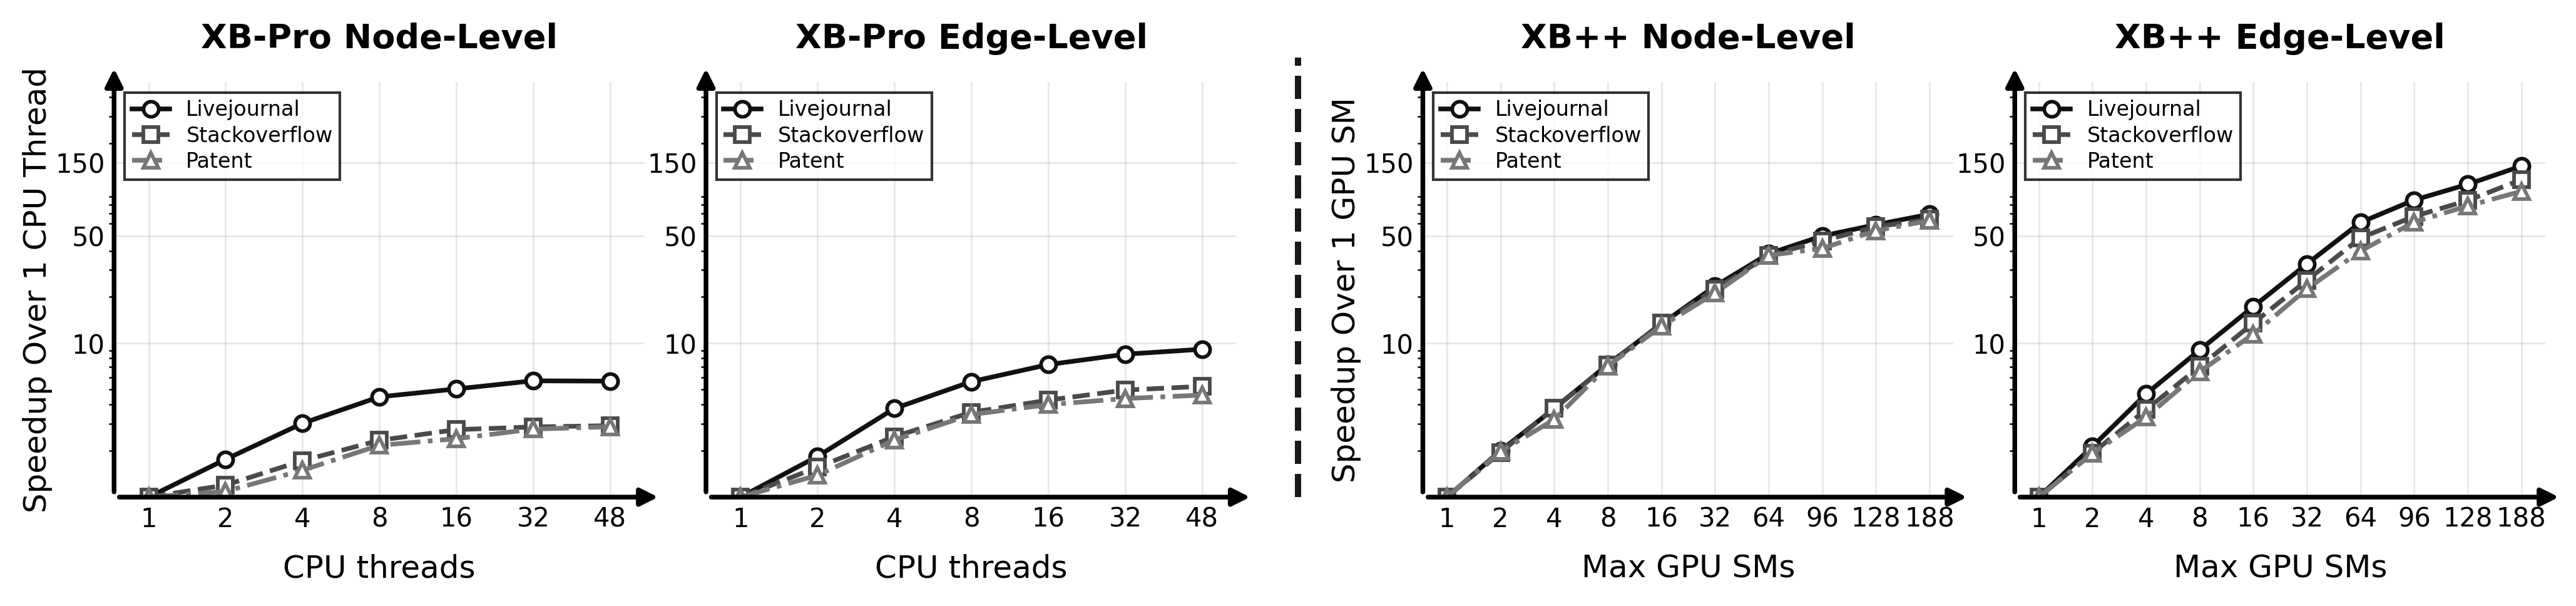
\includegraphics[width=1.0\columnwidth]{figures/plots/plot_scalability.png}
    \captionsetup{skip=4pt}
    \caption{Scalability of XB-Pro and XB++ over one CPU thread or one GPU SM.}
    \label{plot:scalability_test}
\vspace{-4pt}
\end{figure}

\textcolor{blue}{
On both CPU and GPU, edge-level load balancing achieves higher speedups than node-level load balancing on each dataset.
This is because edge-level scheduling exposes finer-grained frontier work, which improves utilization of available execution resources and reduces load imbalance across vertices with different degrees.
The GPU speedups are substantially higher than the CPU speedups as more resources are enabled.
XB++ benefits more from additional GPU SMs because CUDA threads are lightweight and scheduled in warps by hardware, allowing many fine-grained edge tasks to run concurrently and \textcolor{blue}{reduce} amortized memory latency with relatively low scheduling overhead.
In contrast, XB-Pro is limited by the smaller number of CPU cores, heavier software threads, and more expensive synchronization and memory-hierarchy effects, so additional CPU threads provide less aggregate parallel throughput.
}


\section{Architecture Suitability Determination based on Resource Utilization}
\label{sec:arch_suitability}
Multi-core CPUs and GPUs represent distinct architectural trade-offs: CPUs have complex cores for fast multi-threaded execution, while GPUs rely on a large number of simple CUDA cores to achieve massive parallelism.
Accordingly, multi-core CPUs and GPUs achieve high performance in fundamentally different ways: CPUs reduce latency via complex hardware mechanisms and large caches, while GPUs \textcolor{blue}{reduce} amortized latency through massive parallelism.
Recent studies have largely emphasized GPU acceleration for parallel applications; however, such studies face two limitations.
First, GPUs are not a one-size-fits-all solution for all workloads.
Second, multi-core CPUs offer advanced architectural features that enable high performance, including out-of-order superscalar execution, deep pipelining, branch prediction, and large shared L3 caches in addition to per-core L1 and L2 caches.
The effectiveness of these hardware resources is highly workload-dependent.
In this section, we introduce a profiling-based approach and present case studies of four representative traversal-based graph primitives, BFS, SSSP, MSSP, and the blossom algorithm, to assess their architectural suitability. 
This enables informed decisions on whether a traversal-based graph workload is better suited to multi-core CPUs or GPUs.

\subsection{Baselines.}
\label{subsec:baselines}
% In addition to the original X-Blossom implementation, X-Blossom-Pro, and X-Blossom++, we evaluate and profile breadth-first search (BFS) implementations on both CPU and GPU using two state-of-the-art graph processing frameworks: Ligra \cite{shun2013ligra} and Gunrock \cite{wang2016gunrock}. 
% We denote these BFS implementations as BFS-Ligra and BFS-Gunrock, respectively.
In addition to XB-Pro and XB++, we evaluate and profile three representative traversal-based graph primitives, BFS, SSSP, and MSSP, on both CPUs and GPUs using two state-of-the-art graph processing frameworks, Ligra \cite{shun2013ligra} and Gunrock \cite{wang2016gunrock}.
For MSSP, we randomly select source vertices equal to 5\% of all graph nodes.
We denote these implementations by their algorithm and framework, e.g., BFS-Ligra and BFS-Gunrock.
% Why do we need BFS?
These baselines serve as complementary case studies through which we apply our profiling-based methodology introduced in \S~\ref{sec:arch_suitability} and demonstrate its effectiveness in explaining traversal behavior, identifying the dominant performance bottlenecks, and guiding architecture selection between multi-core CPUs and GPUs.

% Ligra and Gunrock
Both Ligra and Gunrock are open-source frameworks that have been actively updated since their first releases.
Ligra is a shared-memory graph processing framework designed for multi-core CPUs, whereas Gunrock is a GPU-based graph analytics framework.
\textcolor{blue}{In our baselines, Ligra parallelizes traversal operators with OpenMP, while Gunrock executes traversal kernels through its CUDA-based graph analytics runtime.}
% Why
Although some prior work has reported traversal implementations that outperform Ligra (e.g., \cite{zhang2018graphit}) and Gunrock (e.g., \cite{wang2019sep}) on particular datasets under architecture-specific optimizations, we deliberately select Ligra and Gunrock as baselines because they remain in active use and development and are widely adopted as reference implementations in prior graph processing studies \cite{zhang2018graphit, nguyen2013lightweight, zhu2016gemini, wang2016gunrock, wang2019sep, brahmakshatriya2021compiling}.
Moreover, both frameworks adopt abstraction models that closely align with the BSP model, making their implementations highly comparable despite targeting different architectures.
Their respective publications also provide direct CPU-GPU comparisons, which serve as established reference points that support the credibility of our experimental results and reinforce the validity of our conclusions.

% In these systems, traversal-based graph primitives have been parallelized in either shared-memory systems, including multi-core CPU frameworks \cite{shun2013ligra, zhang2018graphit, nguyen2013lightweight} and GPU-accelerated frameworks \cite{wang2019sep, wang2016gunrock, brahmakshatriya2021compiling, ben2017groute, wang2023hytgraph, wang2025towards}, or distributed systems that span many machines \cite{gonzalez2012powergraph, malewicz2010pregel, zhu2016gemini, low2012distributed, chen2019powerlyra, gonzalez2014graphx}.
% Amazon and Patent have low Max~Deg, which limits their parallelism exploitation.

% \subsection{Two Traversal Characterization Dimensions}
\subsection{Our Profiling Approach for Traversal-Based Graph Primitives}
\label{subsec:profiling_method}
% The performance of traversal-based graph primitives is strongly influenced by the complex interactions between workload irregularity and architectural resources.
% Graph traversals inherently generate irregular memory-access patterns and uneven parallel workloads, while the underlying platform’s memory hierarchy and execution model determine how efficiently these accesses are handled and how much parallelism can be sustained.
\phantomsection\label{para:metric-selection-justification}
% Citation support:
% graphit_gpu: "The performance of graph programs depends highly on the algorithm, the size and structure of the input graphs"
% wang2016gunrock: "the irregularity of data access and control flow"
% green2019memorychannels: "Graph processing is typically considered to be a memory-bound rather than compute-bound problem."
% beamer2016understanding: "low arithmetic intensity that underutilizes available hardware platforms"
% beamer2015gail: "a single metric cannot be used, and instead it should be complemented by other metrics."
% mukkara2017cache: "limited bandwidth and long latency of main memory accesses"
% beamer2013direction: "As the frontier reaches its largest size, the percentage of peer edges dominates."
% bfs_levelsync: "memory accesses and work distribution are both irregular and data dependent."
\textcolor{blue}{
The performance of traversal-based graph primitives is determined by the interaction among algorithmic structure, input-graph properties, and architectural features \cite{graphit_gpu}.
    In contrast to dense linear-algebra kernels, traversal algorithms such as BFS, SSSP, MSSP, and blossom perform relatively few arithmetic operations per memory access; their execution is dominated by accesses to sparse graph representations, frontier state, and per-vertex or per-edge metadata \cite{wang2016gunrock,green2019memorychannels}.
    As a result, peak compute throughput, including FP64, FP32, FP16, and integer throughput, is not by itself a representative measure of the limiting factors for these workloads \cite{beamer2016understanding}.
    Peak memory bandwidth is also insufficient as a standalone indicator, because graph-analytics performance reflects trade-offs among locality, parallelism, and work efficiency \cite{beamer2015gail}.
    On CPUs, the effective cost of memory access depends on whether the active working set is served by the cache hierarchy, particularly the last-level cache, or requires repeated accesses to DRAM \cite{mukkara2017cache}.
    On GPUs, the amount of parallel work is frontier-dependent: some traversal phases expose enough active work to utilize the memory system, whereas others provide insufficient concurrency to saturate bandwidth \cite{beamer2013direction,bfs_levelsync}.
    Consequently, peak memory bandwidth alone cannot capture the effects of cache locality, memory-system utilization, and available parallelism.
}
To explicitly capture these interactions, we characterize traversal execution patterns along two complementary dimensions: \emph{data movement effectiveness} and \emph{parallelism exploitation}.

%Unlike compute-centric kernels (e.g., dense matrix multiplication), which saturate compute pipelines and scale predictably with an architecture’s peak compute throughput,
%traversal-based graph primitives do not admit such a straightforward characterization.
% two dimensions to capture the interaction between workloads and architectures

% Data Movement efficiency
Data movement effectiveness describes how quickly a traversal brings its working set to the compute cores through the memory hierarchy. 
\textcolor{blue}{The working set refers to the amount of memory that a process requires to complete its execution. For example, BFS requires $O(N)$ memory for the visited array, whereas X-Blossom requires $O(N^2)$ memory for the path table.}
%This dimension is central for traversal-based graph analytics because they typically exhibit low arithmetic intensity, and their performance is therefore primarily dominated by memory accesses rather than arithmetic operations.
%From architectural perspectives, multi-core CPUs and GPUs employ fundamentally different mechanisms to deliver data and tolerate memory latency.
% Parallelism Exploitation
On the other hand, parallelism exploitation characterizes the extent to which a traversal sustains high instruction throughput by maintaining high thread occupancy. On multi-core CPUs, high instruction throughput is achieved through advanced and complex hardware mechanisms, whereas on GPUs it is achieved by exploiting massive parallelism across many simple operations.
Unlike iterative primitives that activate all vertices in every iteration and thus provide consistently high parallelism to exploit, the amount of traversal work is largely determined by the size of the current frontier.
Since the frontier can expand or contract dramatically across iterations, the amount of parallel work available in a traversal can vary widely over time, resulting in highly irregular parallelism.

% Two Types of Profiling Dimensions
% Along these two dimensions, we propose a profiling-based approach that evaluates platform suitability for traversal workloads using a set of characterization measures derived from low-level profiling metrics on multi-core CPUs and GPUs.
Along these two dimensions, we propose a set of characterization measures derived from low-level profiling metrics on multi-core CPUs and GPUs.
On CPUs, we use the L3 cache miss rate and L3 cache miss frequency, namely the \emph{LLC miss rate} and \emph{LLC miss frequency} to reflect how effectively the LLC is utilized, since CPU performance depends strongly on cache behavior to reduce average memory-access latency. 
These two cache-based measures are not applicable on GPUs, where performance is typically dominated by sustained device memory bandwidth and mechanisms that \textcolor{blue}{reduce} effective latency through concurrency.
Accordingly, we use \emph{effective memory bandwidth} to capture the attainable throughput from GPU device memory.
To characterize the parallelism exploitation dimension, we use the \emph{instruction execution rate} on both CPUs and GPUs to quantify how effectively the processor issues and retires instructions given the available parallel work.
Together, these measures indicate whether a traversal workload is primarily constrained by data movement or by limited exploitable parallelism, providing a principled basis for evaluating hardware utilization and platform suitability.


\newcommand{\mcode}[1]{\text{\ttfamily\url{#1}}} % code-ish text that can break
\newcommand{\per}[2]{#1\,/\,#2}

\begin{table}[t]
\centering
\scriptsize
\renewcommand{\arraystretch}{1.1}
\setlength{\tabcolsep}{2pt}
\resizebox{\columnwidth}{!}{%
\begin{tabular}{llll}
\toprule
Platform & Measure & Description & Profiling Counters and Derivation \\
\midrule
CPU & \emph{instruction execution rate} &
Instr./s &
\mcode{instructions} / $t_{\text{exec}}$ \\

CPU & \emph{LLC miss frequency} &
L3 misses/s &
\mcode{mem_load_retired.l3_miss} / $t_{\text{exec}}$ \\

CPU & \emph{LLC miss rate} &
L3 misses/accesses &
\mcode{mem_load_retired.l3_miss} / (\mcode{mem_load_retired.l3_hit} + \mcode{mem_load_retired.l3_miss}) \\
\midrule
GPU & \emph{instruction execution rate} &
Instr./s &
\mcode{sm__sass_thread_inst_executed.sum} / $t_{\text{exec}}$ \\
GPU & \emph{effective memory bandwidth} &
DRAM read bytes/s &
\mcode{dram__bytes_op_read.sum} / $t_{\text{exec}}$ \\
\bottomrule
\end{tabular}%
}
\captionsetup{skip=4pt}
\caption{Five Derived Performance Measures.}
\label{tab:derived-measures}
\vspace{-4pt}
\end{table}


We summarize all derived measures in Table~\ref{tab:derived-measures}. 
The last two columns describe each measure and show how it is computed from the profiling counters used in our scripts.
In addition to the execution time $t_{\text{exec}}$, we collect CPU metrics using \texttt{perf}, the standard Linux performance profiling tool that exposes hardware performance counters, and GPU metrics using NVIDIA Nsight Compute (\texttt{ncu}), a GPU profiling tool that reports low-level kernel counters.
% CPU
On CPUs, the \emph{instruction execution rate} is derived from \emph{instructions}, which counts retired instructions, and is normalized by $t_{\text{exec}}$. 
To characterize CPU data movement, we use the Intel events \emph{mem\_load\_retired.l3\_miss} and \emph{mem\_load\_retired.l3\_hit}, which count retired loads that miss or hit in the L3 cache. 
The LLC miss rate is computed as misses divided by LLC accesses, and the LLC miss frequency is computed as misses divided by $t_{\text{exec}}$. Together, these measures reflect how effectively the LLC captures reuse and reduces DRAM traffic.
% GPU
On GPUs, the \emph{instruction execution rate} is derived from
\emph{sm\_\_sass\_thread\_inst\_executed.sum}, which aggregates the number of instructions executed by active threads across all streaming multiprocessors.
For data movement, we use \emph{dram\_\_bytes\_op\_read.sum}, which reports DRAM read bytes and is normalized by $t_{\text{exec}}$ to obtain effective memory bandwidth.

\subsection{Architectural Suitability of Traversal-Based Graph Primitives}
We now apply our profiling-based methodology to examine hardware resource utilization and to evaluate the architectural suitability of BFS, SSSP, MSSP, and X-Blossom. 
Specifically, we profile both CPU and GPU implementations of these primitives introduced in \S~\ref{subsec:baselines}, enabling a comparative analysis across architectures.
% BFS/SSSP/MSSP
On each dataset, BFS-Ligra, SSSP-Ligra, MSSP-Ligra, BFS-Gunrock, SSSP-Gunrock, and MSSP-Gunrock use the same source-node inputs for the corresponding algorithm, selected from the largest connected component of the graph.
% X-Blossom
In accordance with the architecture-dependent load-balancing strategies discussed in \S~\ref{subsubsec:exp_load_balancing}, XB-Pro employs a node-level strategy, whereas XB++ uses edge-level scheduling to better align with GPU execution.
% CPU
On multi-core CPUs, we profile BFS-Ligra, SSSP-Ligra, MSSP-Ligra, and XB-Pro using \emph{perf}, where 
%following a methodology similar to prior work~\cite{zhu2016gemini}. 
each benchmark is executed 20 times, and both runtime and profiling metrics are averaged across runs to mitigate run-to-run variability and obtain stable measurements.
% GPU
On GPUs, we evaluate and profile BFS-Gunrock, SSSP-Gunrock, MSSP-Gunrock, and XB++ using separate runtime and profiling executions to account for the non-negligible overhead introduced by \texttt{ncu}. 
Specifically, each benchmark is executed 20 times without instrumentation to obtain accurate average runtime measurements, and is executed an additional 20 times with \texttt{ncu} instrumentation to collect low-level profiling counters that characterize architectural behavior.
\subsubsection{Runtime Comparison of Four Traversal-Based Algorithms}
\label{subsubsec:runtime-comparison}

The average runtimes of BFS, SSSP, MSSP, and X-Blossom implementations (mean over 20 runs) are reported in Figure~\ref{plot:runtimes}.
SSSP-Ligra and MSSP-Ligra perform well on the three smallest datasets, while the GPU implementations outperform them on the remaining larger graphs. Overall, the GPU speedup trend follows X-Blossom $>$ MSSP $>$ SSSP $>$ BFS, indicating that GPU benefits increase with the amount of exploitable parallel work. These runtime results validate the baseline measurements used in our profiling-based analysis and motivate the need to explain why BFS, SSSP, MSSP, and X-Blossom exhibit different CPU-GPU scaling behavior.
%These results show that GPU execution is not uniformly beneficial across traversal primitives and datasets. XB++ outperforms XB-Pro on all datasets with high speedups, whereas BFS-Ligra is faster than BFS-Gunrock on nearly all datasets except the two largest graphs.

\begin{figure}[t]
    \centering
    \captionsetup{skip=4pt}
    \caption{
    Performance comparison between CPU and GPU graph traversal implementations. The rows show X-Blossom, BFS, SSSP, and MSSP, comparing the CPU implementation (XB-Pro or Ligra) against the GPU implementation (XB++ or Gunrock). Numbers above GPU bars denote CPU runtime divided by GPU runtime; red values indicate cases with no or only negligible speedup.
    }
    \includegraphics[width=1.0\columnwidth]{figures/plots/plot_runtimes.png}
    \label{plot:runtimes}
\vspace{-4pt}
\end{figure}


\subsubsection{Parallelism Exploitation}
\label{subsubsec:pe}

We first examine instruction execution rate for each of the four baselines, serving as an important indicator on how inherent parallelism in each implementation is effectively exploited on both CPU and GPU. 


\begin{table}[h]
\Huge
\centering
\setlength{\tabcolsep}{3pt}
\renewcommand{\arraystretch}{1.0}
\resizebox{\columnwidth}{!}{%
\begin{tabular}{l|cccc|cccc|cccc}
\toprule
 & \multicolumn{4}{c|}{\textbf{CPU}}
 & \multicolumn{4}{c|}{\textbf{GPU}}
 & \multicolumn{4}{c}{\textbf{CPU--GPU Scaling}} \\
\cmidrule(lr){2-5} \cmidrule(lr){6-9} \cmidrule(lr){10-13}
Dataset &
BFS-Ligra &
SSSP-Ligra &
MSSP-Ligra &
XB-Pro &
BFS-Gunrock &
SSSP-Gunrock &
MSSP-Gunrock &
XB++ &
BFS ($\times$) &
SSSP ($\times$) &
MSSP ($\times$) &
XB ($\times$) \\
\midrule
GPlus         & 132.96 & 178.35 & 218.04 & 34.79 & 710.83 & 736.43 & 896.52 & 2729.93 & 5.35$\times$ & 4.13$\times$ & 4.11$\times$ & 78.48$\times$ \\
Twitch        & 119.87 & 150.44 & 199.31 & 20.00 & 535.52 & 562.65 & 626.35 & 1137.65 & 4.47$\times$ & 3.74$\times$ & 3.14$\times$ & 56.89$\times$ \\
Amazon        & 72.99 & 80.73 & 134.44 & 15.32 & 73.89 & 87.73 & 140.80 & 636.42 & 1.01$\times$ & 1.09$\times$ & 1.05$\times$ & 41.55$\times$ \\
HiggsNets     & 88.95 & 41.81 & 49.40 & 13.25 & 826.49 & 876.90 & 968.16 & 2744.16 & 9.29$\times$ & 20.98$\times$ & 19.60$\times$ & 207.05$\times$ \\
Youtube       & 122.64 & 69.97 & 90.62 & 10.17 & 333.79 & 372.13 & 427.21 & 2579.34 & 2.72$\times$ & 5.32$\times$ & 4.71$\times$ & 253.74$\times$ \\
Hyperlink     & 188.97 & 120.81 & 116.35 & 19.32 & 1531.85 & 1578.79 & 1859.72 & 5027.41 & 8.11$\times$ & 13.07$\times$ & 15.98$\times$ & 260.23$\times$ \\
Wikipedia     & 206.16 & 29.17 & 33.12 & 12.08 & 335.23 & 355.55 & 585.73 & 4917.11 & 1.63$\times$ & 12.19$\times$ & 17.68$\times$ & 407.21$\times$ \\
Stackoverflow & 158.46 & 47.96 & 55.59 & 10.29 & 1641.31 & 1671.18 & 2136.65 & 8131.88 & 10.36$\times$ & 34.85$\times$ & 38.43$\times$ & 790.55$\times$ \\
Patent        & 126.17 & 92.77 & 106.45 & 9.82 & 1107.28 & 1191.08 & 2130.77 & 4969.61 & 8.78$\times$ & 12.84$\times$ & 20.02$\times$ & 506.11$\times$ \\
Livejournal   & 153.34 & 62.59 & 81.33 & 14.77 & 2351.82 & 2476.40 & 3991.76 & 5174.86 & 15.34$\times$ & 39.56$\times$ & 49.08$\times$ & 350.38$\times$ \\
\midrule
Average       & 137.05 & 87.46 & 108.46 & 15.98 & 944.80 & 990.88 & 1376.37 & 3804.84 & 6.70$\times$ & 14.78$\times$ & 17.38$\times$ & 295.22$\times$ \\
\bottomrule
\end{tabular}
}
\captionsetup{skip=4pt}
\caption{
Comparison of instruction execution rates for BFS, SSSP, MSSP, and X-Blossom variants on CPUs and GPUs.
Instruction execution rates are reported in GIPS.
CPU--GPU scaling reports the instruction throughput improvement when migrating execution from CPU to GPU.
Rows follow increasing node count.
}
\label{tab:pe}
\vspace{-4pt}
\end{table}




% ==========================================================================
% Comparison across traversal primitives on the same platform
The CPU and GPU column groups in Table~\ref{tab:pe} compare the instruction execution rates of BFS, SSSP, MSSP, and X-Blossom on the same hardware platform.
%highlighting how each algorithm exploits available parallelism on CPUs and GPUs.
% CPU
On multi-core CPUs, the Ligra implementations of BFS, SSSP, and MSSP all achieve higher average instruction execution rates than XB-Pro, with averages of 137.05, 87.46, and 108.46 GIPS compared with 15.98 GIPS for XB-Pro.
This indicates that the conventional traversal primitives sustain substantially higher CPU instruction throughput than X-Blossom on the evaluated datasets.
Their higher instruction issue rates stem from smaller $O(n)$ per-vertex state and simpler per-frontier operations, which let out-of-order CPU cores find ready instructions and benefit from cache-served memory accesses.
% Why XB-Pro's instruciton exection rate is low.
In contrast, XB-Pro has a much larger working set, dominated by its $O(n^2)$ path table, increasing cache pressure.
Moreover, its node-level load-balancing strategy, though effective for complex operations such as augmenting-path discovery, alternating-tree expansion, and blossom handling, exposes limited parallelism on CPUs. 
This effect is evidenced in Figure~\ref{plot:inst_ratio}, where the node-level strategy consistently attains a lower instruction issue rate on CPUs than the edge-level strategy.
%As a result, the available parallel work is insufficient to fully occupy CPU cores, leading to lower sustained instruction execution rates.
\begin{figure}[t]
    \centering
    \captionsetup{skip=4pt}
    \caption{Instruction issue rate of XB-Pro under node- and edge-level load balancing strategies; numbers above edge bars show the amplification factor (edge-level rate by node-level rate).}
    
\includegraphics[width=1.0\columnwidth]{figures/plots/plot_inst_ratio.png}
    \label{plot:inst_ratio}
\vspace{-8pt}
\end{figure}

% comparison between BFS, SSSP, and MSSP
Another CPU-side observation is that the three traversal baselines, BFS, SSSP, and MSSP, exhibit different instruction-rate trends as dataset size changes.
On small datasets such as GPlus, Twitch, and Amazon, the active state of SSSP and MSSP fits the LLC more effectively, consistent with their lower LLC miss rates in Table~\ref{tab:memory}; as a result, their additional per-vertex update instructions beyond BFS-style traversal can be issued soon after the dependent memory loads complete.
Because MSSP additionally exposes independent frontier work from multiple sources, the small-dataset ordering is MSSP $>$ SSSP $>$ BFS.
On larger datasets, reduced LLC residency increases dependent-load latency in SSSP and MSSP, causing their extra instructions to stall more often behind memory accesses.
BFS therefore often sustains a higher instruction rate through straightforward adjacency scans, while MSSP remains above SSSP because of more parallel frontier work.

%%%%%%%%%%%%%%%%%%%%%%%%%%%%%%%%%%%%%%%%%%%%%%%%%%%%%%%%
% XB-Pro Inst Rate for Node / Edge

% GPU
\phantomsection\label{para:inst_gpu}
On GPUs (see the middle column block under GPU in Table~\ref{tab:pe}), the performance results are largely reversed: 
\textcolor{blue}{XB++ achieves the highest instruction issue rate on all evaluated graphs, with an average of 3804.84 GIPS compared with 944.80, 990.88, and 1376.37 GIPS for BFS-Gunrock, SSSP-Gunrock, and MSSP-Gunrock, respectively.}
% X-Blossom++ (XB++) sustains higher instruction execution rates than BFS-Gunrock on most datasets, with GPU-side ratios exceeding 1$\times$ in the majority of cases and an average speedup of about 2.43$\times$ in this table. 
This improved performance reflects both XB++'s ability to expose more exploitable parallelism through a fine-grained load balancing strategy and the GPU's capacity to maintain high occupancy and hide branching and synchronization overhead via massive multithreading. 
XB++ exposes high parallelism because it activates many vertices concurrently in the initial stage, and repeated clearing and rebuilding of alternating trees regenerates substantial parallel work.
Although BFS and SSSP both start from one source, GPU warp scheduling lets SSSP's extra update work proceed from ready resident warps while other warps wait on memory.
MSSP further increases parallelism by starting from many sources, yielding the ordering XB++ $>$ MSSP-Gunrock $>$ SSSP-Gunrock $>$ BFS-Gunrock across all datasets in Table~\ref{tab:pe}.

These four traversal baselines also show different CPU and GPU trends because their bottlenecks differ by architecture.
On CPUs, smaller datasets such as GPlus, Twitch, and Amazon let the active working set fit more effectively in the LLC; therefore, SSSP, MSSP, and XB-Pro generally achieve higher instruction rates on smaller datasets than on larger ones.
On GPUs, however, the trend reverses: issue rate is driven mainly by available parallelism,
so larger datasets expose more concurrent work and sustain higher rates, while small graphs often underutilize the GPU.

% ==========================================================================
% Migration from CPU to GPU
The CPU--GPU scaling columns of Table~\ref{tab:pe} report instruction-rate scaling when migrating from CPU to GPU execution for all four primitives. 
On average, X-Blossom achieves a 295.22$\times$ instruction-rate scaling, substantially higher than BFS (6.70$\times$), SSSP (14.78$\times$), and MSSP (17.38$\times$), indicating that X-Blossom benefits more substantially from GPU execution.

% This superior scaling stems from X-Blossom’s ability to expose abundant fine-grained parallelism via its edge-level load-balancing strategy: 
% Trend
% Although X-Blossom includes highly-sequential blossom operations, which can limit the parallel efficiency, their impact can be mitigated on GPUs as graph size grows and more parallelism becomes available. 
% This effect is reflected in the CPU–GPU scaling results for X-Blossom, where larger graphs consistently yield higher scaling ratios, indicating richer exploitable parallel work and improved utilization of GPU resources. 
% While a similar trend can be observed for BFS, it is substantially weaker and exhibits greater variability, underscoring BFS cannot expose sufficient parallelism to fully leverage GPU architectures.
% Conclusion
% Overall, our results demonstrate that X-Blossom is fundamentally better suited to GPU execution than CPU execution with the following reasons. 
% Although intricate operations such as blossom handling can reduce parallel efficiency, X-Blossom simultaneously exposes substantially richer fine-grained parallelism, enabling GPUs to hide these overheads and achieve higher hardware utilization. 
% In contrast, despite its straightforward execution pattern, BFS exposes limited parallelism and therefore benefits much less from GPU architectures.

\subsubsection{Data Movement Effectiveness}
In this section, we examine the \emph{LLC miss rate} and \emph{LLC misses frequency} on CPUs for BFS-Ligra, SSSP-Ligra, MSSP-Ligra, and XB-Pro as indicators of how effectively each implementation leverages the large LLC to reduce memory-access latency. 
In contrast, on GPUs we use \emph{effective memory bandwidth} for BFS-Gunrock, SSSP-Gunrock, MSSP-Gunrock, and XB++ to capture how efficiently each implementation utilizes massive concurrency to \textcolor{blue}{reduce} effective memory latency and sustain high device-memory throughput.

\begin{table}[h]
\Huge
\centering
\setlength{\tabcolsep}{3pt}
\renewcommand{\arraystretch}{1.0}
\resizebox{\columnwidth}{!}{%
\begin{tabular}{l|cccc|cccc|cccc}
\toprule
 & \multicolumn{4}{c|}{\textbf{CPU LLC Miss Rate (\%)}}
 & \multicolumn{4}{c|}{\textbf{CPU LLC Miss Freq. (MillMiss/s)}}
 & \multicolumn{4}{c}{\textbf{GPU Effective Memory Bandwidth (GB/s)}} \\
\cmidrule(lr){2-5} \cmidrule(lr){6-9} \cmidrule(lr){10-13}
Dataset &
BFS-Ligra &
SSSP-Ligra &
MSSP-Ligra &
XB-Pro &
BFS-Ligra &
SSSP-Ligra &
MSSP-Ligra &
XB-Pro &
BFS-Gunrock &
SSSP-Gunrock &
MSSP-Gunrock &
XB++ \\
\midrule
GPlus         & 8.07 & 1.05 & 1.01 & 0.38 & 14.62 & 10.09 & 10.64 & 0.44 & 31.22 & 47.19 & 57.83 & 53.79 \\
Twitch        & 1.27 & 0.53 & 0.53 & 0.47 & 6.08 & 3.67 & 4.87 & 0.79 & 24.11 & 37.22 & 40.98 & 42.20 \\
Amazon        & 0.02 & 0.02 & 0.02 & 0.15 & 0.06 & 0.08 & 0.16 & 0.44 & 7.71 & 11.62 & 15.97 & 49.05 \\
HiggsNets     & 4.67 & 1.66 & 2.59 & 0.84 & 5.42 & 2.08 & 3.52 & 1.71 & 37.80 & 57.54 & 62.76 & 98.97 \\
Youtube       & 0.39 & 0.26 & 0.34 & 1.47 & 0.73 & 0.51 & 0.74 & 3.49 & 21.45 & 32.38 & 40.28 & 195.84 \\
Hyperlink     & 6.97 & 2.55 & 2.70 & 5.97 & 32.56 & 10.85 & 11.60 & 22.68 & 73.77 & 110.64 & 126.66 & 251.92 \\
Wikipedia     & 2.17 & 2.82 & 3.53 & 5.63 & 4.76 & 3.15 & 3.40 & 10.08 & 21.74 & 32.57 & 52.23 & 258.48 \\
Stackoverflow & 6.17 & 1.47 & 1.60 & 7.58 & 73.47 & 12.49 & 14.09 & 25.87 & 83.45 & 123.36 & 159.40 & 343.14 \\
Patent        & 4.37 & 2.41 & 2.41 & 7.82 & 78.63 & 45.88 & 41.43 & 33.15 & 75.35 & 116.81 & 198.44 & 424.13 \\
Livejournal   & 27.05 & 3.07 & 3.16 & 13.52 & 112.55 & 18.32 & 23.74 & 63.15 & 123.45 & 188.33 & 314.74 & 520.45 \\
\midrule
Average       & 6.12 & 1.58 & 1.79 & 4.38 & 32.89 & 10.71 & 11.42 & 16.18 & 50.01 & 75.77 & 106.93 & 223.80 \\
\bottomrule
\end{tabular}
}
\captionsetup{skip=4pt}
\caption{
Comparison of CPU cache behavior and GPU memory bandwidth for BFS, SSSP, MSSP, and X-Blossom variants.
CPU metrics report LLC miss rate and LLC miss frequency in million misses per second, while GPU metrics report effective memory bandwidth.
Rows follow increasing node count.
}
\label{tab:memory}
\vspace{-4pt}
\end{table}


% ==========================================================================
% CPU-LLC Miss Rate & LLC miss frequency
Table~\ref{tab:memory} reports two CPU-side cache metrics for BFS-Ligra, SSSP-Ligra, MSSP-Ligra, and XB-Pro.
The \emph{LLC miss rate} measures the fraction of missed accesses to LLC, while \emph{LLC misses frequency} captures the absolute rate of LLC misses during execution. 
Together, these metrics characterize how effectively each implementation leverages the last-level cache to reduce memory-access latency. 
On average, SSSP-Ligra and MSSP-Ligra have the lowest LLC miss rates (1.58\% and 1.79\%) and miss frequencies (10.71 and 11.42 million misses/s), while XB-Pro has a lower average miss rate than BFS-Ligra (4.38\% vs. 6.12\%) and a lower average miss frequency (16.18 vs. 32.89 million misses/s). %suggesting more effective cache utilization.
Overall, both CPU cache metrics follow BFS $>$ XB-Pro $>$ SSSP/MSSP.
BFS issues sparse adjacency accesses with little per-edge computation, so it generates LLC misses quickly.
SSSP and MSSP spend more time on relaxation and distance updates between memory requests; XB-Pro falls between them because blossom processing reuses fetched path-table data despite $O(n^2)$ path-table pressure.

% 2. GPU-Effective Memory Bandwidth
On GPUs, XB++ achieves the highest average effective memory bandwidth, 223.80 GB/s, compared with 50.01, 75.77, and 106.93 GB/s for BFS-Gunrock, SSSP-Gunrock, and MSSP-Gunrock, respectively. 
This shows the benefit of XB++'s edge-level parallelism.
By exposing substantially more concurrency than BFS, SSSP, and MSSP, XB++ keeps more warps active and sustains a higher memory request rate, which helps \textcolor{blue}{reduce} amortized latency and enables more effective utilization of the GPU's high-bandwidth memory system.
The main exception is GPlus, where MSSP-Gunrock slightly exceeds XB++ in effective bandwidth, because GPlus has the highest blossom density and the resulting blossom handling introduces control-flow and synchronization work that limits XB++'s memory-bandwidth utilization.

% 3. Conclusion
To summarize, these memory results show that X-Blossom has competitive CPU cache behavior relative to SSSP/MSSP and substantially higher GPU memory-bandwidth utilization than all Gunrock traversal baselines.
On CPUs, XB-Pro improves efficient LLC utilization through increased data reuse, while on GPUs, XB++ better harnesses its abundant parallelism to sustain higher effective memory bandwidth.

\subsubsection{Our Findings and general recommendations}
% Parallelism is all you need
The degree of exploitable parallelism largely determines whether migrating BFS, SSSP, MSSP, or X-Blossom from CPU to GPU is beneficial.
% X-Blossom
On CPUs, XB-Pro leverages the LLC effectively for its high locality. 
Migrating to GPUs diminishes these cache-related benefits and exposes the overheads of complex and sequential blossom operations. 
Nevertheless, X-Blossom provides substantial fine-grained parallelism, allowing XB++ to keep a large number of warps active and effectively \textcolor{blue}{reduce} effective memory latency, overcoming these drawbacks to achieve significant GPU speedups over CPU execution. Thus, XB++ is best fit on GPU for high performance.  

% BFS
In contrast, BFS, SSSP, and MSSP execute simpler traversal operations and sustain substantially higher instruction throughput on CPUs than XB-Pro.  
%so moving away from cache-centric execution tends to incur a smaller penalty
%Moreover, BFS is dominated by simple graph-traversal operations, which are, in principle, well suited to GPU execution.
When migrated to GPUs, their benefits vary with the amount of frontier-level parallelism. 
BFS shows the weakest average instruction-rate scaling (6.70$\times$), while SSSP and MSSP achieve higher but still moderate scaling (14.78$\times$ and 17.38$\times$), far below X-Blossom's 295.22$\times$ scaling. 
As a result, these conventional traversal primitives are less uniformly GPU-favorable than X-Blossom in our measurements; BFS in particular often achieves limited or even negative runtime gains on GPUs, which is consistent with prior CPU-focused BFS optimization work \cite{shun2015ligraplus,zhang2018graphit}.

% Conclusion 
The case studies presented in this paper can be generalized to other applications using our profiling-based methodology.
Based on our analysis of parallelism exploitation, data-movement efficiency, and observed runtime results in this study, we articulate the following guiding principle to address the architectural suitability. Workloads exhibiting high degrees of parallelism in both computation and data movement benefit significantly more from GPU architectures than from multi-core CPUs, as reflected by high instruction issue rates and high effective memory bandwidth on GPUs. In contrast, workloads with relatively limited parallelism and small working sets of high locality are better suited to multi-core CPUs, which can achieve high performance by effectively exploiting complex core micro-architectures and deep memory hierarchies.


\section{Related Work}
%%%%%%%%%%%%%%%%%%%%%%%%%%%%%%%%%%%%%%%%%%%%%%%%%%%%%%%%%%%
% Blossom algorithm
% Sequential versions
\textbf{Blossom Algorithms.}
The blossom algorithm~\cite{edmonds1965paths} is foundational for computing maximum matchings in general graphs. Subsequent work improves its sequential performance through optimized data structures and algorithmic refinements~\cite{gabow1976efficient, gabow1984efficient, gabow1990data, gabow1991faster, blum2015maximum}. Despite these advances, Edmonds’ algorithm remains the dominant practical framework.
% Parallel versions
Parallel implementations have also been explored~\cite{Stanford_2016, Wayne_2024, fan2025x}. Among them, X-Blossom removes recursion and reformulates blossom handling, enabling GPU-oriented implementations of maximum matching in general graphs.

%%%%%%%%%%%%%%%%%%%%%%%%%%%%%%%%%%%%%%%%%%%%%%%%%%%%%%%%%%%
% BFS
\noindent
\textbf{BFS.}
As a fundamental graph traversal primitive, BFS has been studied extensively.
Most systems implement BFS in a level-synchronous manner, advancing a frontier level by level~\cite{bfs_levelsync}.
Direction-optimizing BFS (DOBFS) improves performance by switching between top-down push and bottom-up pull to reduce redundant edge examinations~\cite{beamer2011searching,beamer2013direction}. Subsequent work improves frontier representations (sparse vs.\ dense)~\cite{bfs_standford,shun2013ligra,shun2015ligraplus}, reduces contention (e.g., bitmap visited states and fewer atomics)~\cite{bfs_agarwal}, and enhances locality and scalability via frontier reordering and NUMA-aware scheduling~\cite{bfs_locality,bfs_numa,zhang2015numa,arai2016rabbit}. Related implementations appear across distributed systems (Pregel~\cite{malewicz2010pregel}, GraphLab~\cite{low2012graphlab}, PowerGraph~\cite{gonzalez2012powergraph}, Gemini~\cite{zhu2016gemini}), shared-memory CPU frameworks (Galois~\cite{nguyen2013galois}, Ligra/Ligra+~\cite{shun2013ligra,shun2015ligraplus}, Julienne~\cite{ligra_julienne}, Aspen~\cite{ligra_aspen}), and GPU frameworks (Gunrock~\cite{wang2016gunrock}, Groute~\cite{ben2017groute}, Lux~\cite{jia2017lux}, SEP-Graph~\cite{wang2019sep}). Finally, several systems auto-tune these choices for hardware- and graph-specific implementations~\cite{zhang2018graphit,graphit_ordered2020,graphit_gpu,graphit_novelarch}.

%%%%%%%%%%%%%%%%%%%%%%%%%%%%%%%%%%%%%%%%%%%%%%%%%%%%%%%%%%%
% SSSP
\noindent
\textcolor{blue}{\textbf{SSSP and MSSP.}
SSSP extends BFS-style traversal to weighted graphs and is commonly optimized around the tension between priority ordering, redundant work, and exposed parallelism.
Classical approaches include Dijkstra's priority-ordered algorithm and parallel Dijkstra variants~\cite{dijkstra1959note,crauser1998parallelization}, while $\Delta$-stepping uses bucketed relaxation to trade exact priority order for parallel work~\cite{meyer2003delta}.
Subsequent multicore SSSP techniques refine this trade-off through radius/stepping variants, DSMR, relaxed priority schedulers such as SprayList and MultiQueues, and Wasp's priority-aware work stealing~\cite{blelloch2016radius,maleki2016dsmr,dong2021efficient,alistarh2015spraylist,rihani2015multiqueues,postnikova2022multiqueues,dantonio2025wasp}.
SSSP implementations also appear in GAP, GBBS, Galois, Ligra, Gunrock, and GraphIt, where scheduling choices balance locality, synchronization, load balance, and redundant relaxation~\cite{azad2020gap,dhulipala2021gbbs,nguyen2013galois,shun2013ligra,wang2016gunrock,zhang2018graphit}.
On GPUs, work-efficient methods such as Workfront Sweep, Near-Far, and Bucketing reduce redundant relaxation while exposing parallel work~\cite{davidson2014work}; later GPU SSSP work improves scheduler and worklist quality through asynchronous dynamic $\Delta$-stepping, bucket-aware execution, dynamic-stepping heuristics, and multi-level multi-queue designs~\cite{wang2021fastsssp,zhang2023bucketaware,yu2025heuristic,hu2026mlmq}.}

%%%%%%%%%%%%%%%%%%%%%%%%%%%%%%%%%%%%%%%%%%%%%%%%%%%%%%%%%%%
% MSSP
\textcolor{blue}{MSSP has been studied as both a planar-graph primitive and batched SSSP in general graph analytics.
Planar-graph MSSP techniques compactly represent shortest-path trees for all boundary-face sources and compute distances from those roots ~\cite{klein2005multiple}.
This line of work has also been extended to embedded-graph MSSP and linear-time algorithms for unit-weight planar MSSP~\cite{cabello2013multiple,eisenstat2013linear}.
Beyond these specialized techniques, general graph analytics often treats MSSP as batched shortest-distance computation, using batched Dijkstra and Bellman--Ford variants~\cite{then2017batched}.
This batched view also aligns with frameworks supporting MSSP through frontier-based traversal operators and scheduling abstractions~\cite{shun2013ligra,wang2016gunrock,zhang2018graphit}.}

%%%%%%%%%%%%%%%%%%%%%%%%%%%%%%%%%%%%%%%%%%%%%%%%%%%%%%%%%%%
% CPU and GPU analysis => Debunking
\noindent
\textbf{The Platform Selection.}
%The CPU versus GPU detbate has remained heated for more than two decades. 
% GPU is fast
With programmable GPUs, many domain experts rewrote performance-critical kernels for massive parallelism and reported striking speedups across diverse domains such as networking ~\cite{gpu_network_1,gpu_network_2}, databases analytics ~\cite{gpu_db_1,gpu_db_2}, and classic algorithmic primitives ~\cite{gpu_algo_1,gpu_algo_2}. 
However, early claims of substantial GPU performance advantages ~\cite{gpuIsFast_che,gpuIsFast_ryoo} motivated systematic CPU-GPU comparisons. 
% CPU
Meanwhile, CPUs have continued to evolve, adopting wider SIMD vectors~\cite{cpu_simd_1,cpu_simd_2} and integrating higher-bandwidth memory technologies~\cite{cpu_hbm_1,cpu_hbm_2}. 
Recent CPU-centric studies also report strong performance and energy efficiency across modern scientific and memory-bound workloads~\cite{cpu_perf_1}, and in some cases, CPU kernels can even rival or outperform GPU counterparts~\cite{cpu_over_gpu_1,cpu_over_gpu_2,cpu_over_gpu_3}.
% Platform Selecition
%These ongoing comparisons have motivated more rigorous CPU–GPU evaluations that emphasize architecture-aware optimization and insightful interpretation metrics, rather than relying on raw runtime speedups alone.
A study has reexamined early reports of dramatic GPU gains~\cite{gpuIsFast_che,gpuIsFast_ryoo}, showing that many such speedups shrink markedly when CPU and GPU implementations are optimized to a comparable level and evaluated fairly with respect to architectural constraints~\cite{lee2010debunking}.
The importance of including host--device data transfer overheads in end-to-end measurements is also emphasized ~\cite{gregg2011transfer}. 
Power and energy efficiency have also been studied to inform system design~\cite{gpu_energy}, while newer interpretation metrics (e.g., peak-based crossover) help determine when GPUs outperform CPUs for batch workloads~\cite{peek_metrics2025}.
Finally, standardized benchmark suites support comparable cross-platform evaluation, including GAP for graph analytics~\cite{benchmark_gap,benchmark_gap_eval} and MLPerf for machine learning~\cite{benchmark_mlperf,benchmark_mlperfhpc}. 

%These related efforts focus on software-level optimizations and are largely case-specific. In contrast, our profiling metrics capture critical architectural factors governing program execution, quantify hardware resource utilization, and assess workload suitability for either multicore CPUs or GPUs.
All of the aforementioned related efforts focus on software-level optimizations and are largely case-specific. In contrast, our profiling metrics capture the critical architectural factors governing program execution, quantifying hardware resource utilization levels and enabling a systematic assessment of workload suitability for either multicore CPUs or GPUs.


\section{Conclusion}
In this study, we focus on four representative traversal-based graph analytics workloads: BFS, SSSP, MSSP, and the blossom algorithm by developing an enhanced multi-core CPU implementation of blossom (X-Blossom-Pro) and a highly optimized GPU implementation (X-Blossom++). We propose a set of profiling metrics to systematically measure and analyze performance, providing insights into workload behavior on the two platforms. By examining execution patterns on both multi-core CPUs and GPUs, we identify several critical issues in the interaction between graph analytics workloads and underlying architectures, particularly from the perspective of resource utilization. Our approach enables informed architectural decisions for achieving high performance not only in traversal-based graph analytics but also in general parallel applications, either by leveraging the sophisticated hardware mechanisms and deep memory hierarchies of multi-core CPUs or by exploiting massive parallelism across large numbers of CUDA cores on GPUs.


\newpage
%%
%% The next two lines define the bibliography style to be used, and
%% the bibliography file.
\bibliographystyle{ACM-Reference-Format}
\bibliography{sample-base}

%%
%% If your work has an appendix, this is the place to put it.
\clearpage
\appendix

\begin{figure*}[h]
  \centering
  {\Large\bfseries\sffamily Resubmission of SIGMETRICS-26-WINTER Submission \#210}
  % \vspace{2pt}
  % \caption*{}  
\end{figure*}

We sincerely thank all reviewers and the PC for their comprehensive and insightful comments.
We have carefully revised the paper following their constructive suggestions.
In this appendix, Section~\ref{sec:major-revisions} summarizes the revisions made in response to the major comments, Section~\ref{sec:specific-replies} provides specific replies to each reviewer, and Section~\ref{expr:ci_tables} reports supplementary confidence-interval tables for the revised experiments.

\section{Revisions Following Major Comments}
\label{sec:major-revisions}

\subsection{Clarify the contributions, especially on the implementation side}
\label{subsec:rev-contributions}
We added implementation details for X-Blossom-Pro and X-Blossom++ to the first two items in the contribution list in Subsection~\ref{subsec:intro-exec-summary}.

\subsection{Include more details of the experimental setup}
\label{subsec:rev-exp-setup}
We expanded the experimental setup description to include the cloud platform, operating system, instance types, processor and accelerator models, CPU core/thread counts, and the framework/threading model used by each implementation. 
Specifically, we clarified that XB-Pro uses C++ \texttt{std::thread} with pthread support and XB++ uses CUDA kernels; for the Ligra and Gunrock baselines, we state that Ligra uses OpenMP for CPU parallelism and Gunrock runs on a CUDA-based graph analytics framework.
These additions provide a more complete and reproducible description of the hardware and software environment used in the revised experiments. Further details can be found in Subsubsection~\ref{subsubsec:eval-exp-env} and Subsection~\ref{subsec:baselines}.

\subsection{Scalability test}
\label{subsec:rev-scalability}
We added a new scalability experiment that evaluates both XB-Pro and XB++ under node-level and edge-level load-balancing strategies on three graph datasets. 
The results show that edge-level load balancing generally achieves higher speedup than node-level load balancing, and that GPU scaling is higher than CPU scaling due to lower CUDA-thread overhead and efficient SM-level parallel execution.
Further details can be found in the Subsection~\ref{subsec:scalability_test}.

\subsection{Clarify the i9 cores vs. threads}
\label{subsec:rev-cores-threads}
We revised the hardware description to explicitly distinguish physical CPU cores from hardware threads. In the updated setup, the CPU instance is reported as having 48 physical cores and 96 hardware threads, avoiding ambiguity between core count and thread count. Further details can be found in Subsubsection~\ref{subsubsec:eval-exp-env}.

\subsection{Add confidence intervals}
\label{subsec:rev-confidence-intervals}
We added confidence intervals (CIs) to Tables~\ref{tab:graph-metrics} and \ref{tab:reuse} to demonstrate the stability of the reported averages.
For Table~\ref{tab:pe}, Table~\ref{tab:memory}, and Figures~\ref{plot:load-balance}, \ref{plot:scalability_test}, \ref{plot:runtimes}, and \ref{plot:inst_ratio}, we provide the corresponding CI tables in the appendix (Section~\ref{expr:ci_tables}) to keep the main presentation compact and readable.

\subsection{Include details about execution phases}
\label{subsec:rev-execution-phases}
We revised the last two paragraphs of the load-balancing discussion in Subsubsection~\ref{subsubsec:exp_load_balancing}; the revised sequential-work paragraph clarifies which parts of X-Blossom++ remain sequential or expensive~\hyperref[para:xbpp-sequential-work]{(see the sequential-work paragraph)}, and the revised parallel-work paragraph clarifies which major search phases are parallel~\hyperref[para:xbpp-parallel-work]{(see the parallel-work paragraph)}. Together, the revised text explains that CPU-to-GPU speedup is governed by the fraction of work that can be exposed as fine-grained parallel GPU tasks versus the remaining sequential blossom/path-table work, so it does not scale directly with the raw increase in GPU thread count.

\subsection{Run CPU and GPU experiments on comparable platforms}
\label{subsec:rev-fair-platform}
To address this concern, we moved the experiments from the previous local i9/A100 setup to server-class Amazon Web Services (AWS) instances. Although we still used two separate instances because AWS GPU instances do not expose the bare-metal memory-system information required for our CPU baseline evaluation, the comparison is fair because both platforms are server-class AWS instances selected for the corresponding CPU and GPU baselines rather than consumer or mobile hardware. The CPU baselines were evaluated on an m7i.metal-24xl bare-metal instance, a current-generation AWS server-class instance with 4th Generation Intel Xeon processors, which provides direct access to the memory-system information required by our CPU-side analysis. The GPU baselines were evaluated on a server-class AWS GPU instance using an NVIDIA RTX PRO 6000 Blackwell Server Edition GPU, which is newer than the A100-class platform and provides competitive or better performance for the evaluated GPU baselines. Further details can be found in Subsubsection~\ref{subsubsec:eval-exp-env}.

\subsection{Explain why the ratio is small for some larger graphs in Table~5}
\label{subsec:rev-inst-ratio}
This issue no longer appears after moving the experiments from the previous A100 platform to the RTX PRO 6000 Blackwell platform. The A100 exposes 108 SMs, whereas the RTX PRO 6000 Blackwell exposes 188 SMs, providing substantially more SM-level execution resources. With the revised platform, XB++ achieves a higher instruction issue rate than BFS-Gunrock on all evaluated graphs, which is consistent with our conclusion that XB++ exposes more GPU parallelism through fine-grained edge-level work. We updated the first sentence in 
\hyperref[para:inst_gpu]{this paragraph} to explicitly state this observation and connect it to our parallelism-exploitation conclusion.

\subsection{Comment on the variability in the improvement of the speedup across different graphs in Table~\ref{tab:reuse}}
\label{subsec:rev-reuse-variability}
We added one dynamic metric, ReuseRatio, to Table~\ref{tab:reuse} and used it to explain the variability in reuse speedups across graphs in Subsection~\ref{subsub:exp_reuse}. 
ReuseRatio measures the percentage of alternating-tree nodes preserved by the reuse mechanism rather than reset, so it directly captures the internal behavior that alternating-tree reuse is designed to exploit. 
The revised discussion shows that datasets with higher ReuseRatio generally obtain larger speedups.

\subsection{Expand a bit on how SIMT execution helps to keep up massive concurrency}
\label{subsec:rev-simt-concurrency}
We expanded the explanation of SIMT execution to clarify how it helps XB++ maintain massive concurrency and reduce effective memory and control-flow latency, especially when edge-level load balancing exposes enough fine-grained tasks in \hyperref[para:smit_execution]{this paragraph}.

\subsection{Explain small working set a bit more on Page~17}
\label{subsec:rev-working-set}
We added a definition of working set to the data-movement discussion in Subsection~\ref{subsec:profiling_method}.

\section{Specific Replies to Each Reviewer}
\label{sec:specific-replies}

\subsection{Reply to Reviewer-B}

\noindent\textbf{Suggestion B1:} \textit{In several places you write ``hide latency''; maybe it will be better to write ``reduce latency''.} 
\\

\noindent Thank you for the wording suggestion. We have updated all instances of ``hide latency'' and related wording to ``reduce amortized latency'' in the revised manuscript.
\\

\noindent\textbf{Suggestion B2:} \textit{In Ref.~\cite{gonzalez2012powergraph}, \{PowerGraph\} should be PowerGraph and \{Graph-Parallel\} should be Graph-Parallel.}
\\

\noindent Thank you for pointing out this typo. We have corrected Ref.~\cite{gonzalez2012powergraph} by removing the rendered braces around PowerGraph and Graph-Parallel.
\\

\subsection{Reply to Reviewer-C}

\noindent\textbf{Comment C1:} \textit{Unbalanced hardware tiers confound the CPU-GPU suitability claim. The CPU baselines are evaluated on an Intel Core i9-14900HX system, while the GPU baselines run on a separate machine with an NVIDIA Tesla A100. This comparison mixes a mobile-class CPU platform with a data-center-class GPU platform, making it difficult to attribute observed differences to architectural suitability rather than system-class effects (e.g., sustained power limits and, especially, host memory subsystem/bandwidth).}
\\

\noindent Thank you for raising this concern about comparison fairness. In the revised experiments, we moved both the CPU and GPU evaluations to server-class AWS platforms to avoid comparing a mobile-class CPU system against a data-center GPU system. The updated platform choice is summarized in Subsection~\ref{subsec:rev-fair-platform} of Section~\ref{sec:major-revisions}.
\\

\noindent\textbf{Comment C2:} \textit{In addition, the CPU configuration description appears ambiguous (on page 11) (the i9-14900HX is a mobile HX-series part and is commonly specified as 24 cores/32 threads), so clarifying cores vs.\ threads and the threading/pinning policy is important for reproducibility.}
\\

\noindent Thank you for pointing out this ambiguity. We revised the experimental setup to explicitly distinguish CPU cores from hardware threads and to include the relevant CPU architectural details for reproducibility. These clarifications are described in Subsection~\ref{subsec:rev-cores-threads} and Subsection~\ref{subsec:rev-exp-setup} of Section~\ref{sec:major-revisions}.
\\

\subsection{Reply to Reviewer-D}

\noindent\textbf{Comment D1:} \textit{It would be good to explain why the ratio is small (close to 1) for some of the larger graphs in Table 5 (column 6) if enough parallel work is available under XB++?}
\\

\noindent This is an insightful point. After moving the experiments from the A100 platform to the RTX PRO 6000 Blackwell platform, this issue no longer appears: XB++ now achieves a higher instruction issue rate than BFS-Gunrock on all evaluated graphs. The revised results suggest that the earlier near-1 ratios were partly due to limited available SM-level execution resources on the original GPU platform rather than a lack of parallel work in XB++. We address this ratio issue in Subsection~\ref{subsec:rev-inst-ratio} of Section~\ref{sec:major-revisions}.
\\

\noindent\textbf{Comment D2:} \textit{It would be nice to comment on the variability in the improvement of the speedup across different graphs in Table 2.}
\\

\noindent We appreciate the reviewer highlighting this variability. To explain the differences across graphs, we added a new metric, Reuse-Ratio, which measures how effectively the alternating-tree reuse mechanism preserves useful tree nodes instead of resetting them. This metric helps connect the observed speedups in Table~2 to the internal behavior of the reuse optimization. The added explanation of speedup variability is given in Subsection~\ref{subsec:rev-reuse-variability} of Section~\ref{sec:major-revisions}.
\\

\noindent\textbf{Comment D3:} \textit{It would be nice to expand a bit on how SIMT execution helps to keep up massive concurrency (I am not very familiar with this area).}
\\

\noindent This is necessary context for interpreting the GPU performance results. In the revision, we expanded the discussion to explain how resident warps help the GPU maintain high concurrency when XB++ exposes enough fine-grained edge-level work. The added discussion is summarized in Subsection~\ref{subsec:rev-simt-concurrency} of Section~\ref{sec:major-revisions}.
\\

\noindent\textbf{Comment D4:} \textit{Can you please explain small working set a bit more on Page 17: is it related to the amount of memory needed to store required data in cache?}
\\

\noindent This is an important clarification. We added an explicit definition of working set in the data-movement discussion of the profiling methodology. The corresponding revision is summarized in Subsection~\ref{subsec:rev-working-set} of Section~\ref{sec:major-revisions}.
\\

\noindent\textbf{Comment D5:} \textit{Section 2.4 is not very clear: How are the 3 procedures performed parallely? It would be nice to expand on the claim in the introduction that the usual parallel algorithm throws away alternating paths instead of reusing it.}
\\

\noindent We agree that the parallel execution of the three procedures needed a clearer explanation. We added a paragraph in Section~2.4 describing how the current checking set is split across worker threads and how each phase processes its assigned frontier vertices. The added paragraph is marked in \hyperref[para:xblossom-three-parallel-procedures]{this paragraph}.
\\

\noindent\textbf{Comment D6:} \textit{The acronyms CPU and GPU must be expanded the first time it is used in the paper -- same goes for SIMT and LLC.}
\\

\noindent Thank you for catching these acronym issues. We expanded CPU and GPU at their first prose occurrence in \hyperref[para:first-cpu-gpu]{the abstract} and also clarified them in the experimental setup at \hyperref[para:exp-setup-cpu]{the CPU platform description} and \hyperref[para:exp-setup-gpu]{the GPU platform description}. We also expanded LLC at \hyperref[para:first-llc]{its first body-text occurrence} and SIMT at \hyperref[para:first-simt]{its first evaluation occurrence}.
\\

\noindent\textbf{Comment D7:} \textit{Figure~\ref{plot:load-balance} discussion: It would be nice to remind the reader that having blossoms reduces the effectiveness of node-level parallelism as discussed in Subsection~\ref{subsubsec:exp_load_balancing}.}
\\

\noindent This connection helps interpret the load-balancing results. We added the explanation that blossom-heavy workloads involve sequential path-table operations, including tracing endpoint-to-root paths to identify the blossom base and materializing the odd cycle from path segments. The added discussion is marked in \hyperref[para:blossom-node-level-limitation]{this paragraph}.
\\

\noindent\textbf{Comment D8:} \textit{Section~\ref{sec:intensive-experiments} discusses BFS-Ligra and BFS-Gunrock but they are compared only in Section~\ref{sec:arch_suitability}. This discussion could possibly be moved to the start of Section~\ref{sec:arch_suitability}.}
\\

\noindent Thank you for the organization suggestion. The moved discussion is now in Subsection~\ref{subsec:baselines}.
\\

\subsection{Reply to Reviewer-E}

\noindent\textbf{Contribution Concern E1:} \textit{The proposed profiling methodology is not new. It is using well-known common metrics and popular tools. It is a good case study but I think the profiling tehcniques and metrics you proposed are standard procedures. Additionally, the selection of the LLC and memory efficiency needs more scientific justification. How about other metrics? .e.g, LLC occupancy, effective DRAM bandwidth? I think a more careful consideration of the metric space exploration and narrowing down to a limited set of metrics would strength the technical depth of this part.
You claim your contribution in page 3 ``Our performance analysis methodology can be applied to general parallel-processing applications'': I am assuming you are referring to the profiling part. The profiling technique is standard, so I agree that this can be applied to general applications. But this cannot be listed as a contribution. I would recommend using this bullet point to talk about the takeaway messages you obtained from your profiling case study.}
\\

\noindent Thanks for your constructive suggestions.
To justify our selected metrics, we added a paragraph before introducing our measures to explain why commonly reported peak metrics, including peak FP64/FP32/FP16/integer throughput and peak memory bandwidth, do not capture the execution pattern of traversal-based graph workloads.
This metric-selection rationale has been added in \hyperref[para:metric-selection-justification]{this paragraph}.

\noindent We also revised the contribution statement to focus on the architectural-suitability takeaway distilled from the case study. The revised contribution bullet is marked in \hyperref[item:takeaway-architecture-suitability]{this contribution item}.
\\

\noindent\textbf{Contribution Concern E2:} \textit{All the evaluated graphs are sparse. Given that many of the real-world graph networks are sparse, your contribution is still valuable. However, please either tone down your contribution from general graphs to sparse graphs, or you should include dense graph benchmarks in your evaluation.}
\\

\noindent Thank you for this helpful scope clarification.
We revised the dataset description to state explicitly that this paper focuses on real-world sparse graph datasets.
The added clarification is marked in \hyperref[para:real-world-sparse-datasets]{this paragraph}.
\\

\noindent\textbf{Contribution Concern E3:} \textit{The whole paper covers two types of graph algorithms(applications): BFS and blossom, but they are loosely connected. The argument from the authors is that these two algorithms are both graph traversal with frontier-expansion paradigm. Then how about other traversal algorithms? e.g., SSSP?}
\\

\noindent We appreciate this suggestion to strengthen the generality of our performance-analysis approach beyond BFS and blossom. We have already applied it to two additional traversal-based graph algorithms, SSSP and MSSP. Their instruction execution rates are reported in Table~\ref{tab:pe}, and their CPU cache behavior and GPU memory-bandwidth results are reported in Table~\ref{tab:memory}, both in Section~\ref{sec:arch_suitability}.
\\

\noindent\textbf{Evaluation Detail E1:} \textit{What framework/lib are you using for evaluation? For CPU, are you using openMP, or pthread? For the two baselines Ligra and Gunrock, what are they using? These things should be included in the paper to judge that you are doing a fair comparison.}
\\

\noindent Thank you for the question. The added framework and environment details are summarized in Subsection~\ref{subsec:rev-exp-setup} of Section~\ref{sec:major-revisions}. In the main paper, XB-Pro and XB++ parallelization details are given in Subsubsection~\ref{subsubsec:eval-exp-env}, while the Ligra and Gunrock baseline details are given in Subsection~\ref{subsec:baselines}.
\\

\noindent\textbf{Evaluation Detail E2:} \textit{The scalability test is missing. When varying the number of threads, how does the performance trend look like?}
\\

\noindent Thank you for pointing out this. We added a scalability test that varies the number of CPU threads for XB-Pro and the number of enabled GPU SMs for XB++.
The revision is summarized in Subsection~\ref{subsec:rev-scalability} of Section~\ref{sec:major-revisions}, with full details in Subsection~\ref{subsec:scalability_test}.
\\

\noindent\textbf{Evaluation Detail E3:} \textit{The CPU platform uses i9-14900HX, which has 24 cores, not 32 cores. It is 8 performance cores x 2 (SMT) + 16 Efficient cores = 32 threads when SMT (hyperthreading) is enabled.}
\\

\noindent Thank you for the correction. We revised the core/thread description, as documented in Subsection~\ref{subsec:rev-cores-threads} of Section~\ref{sec:major-revisions}.
\\

\noindent\textbf{Evaluation Detail E4:} \textit{Confidence intervals missing.}
\\

\noindent Thank you for the suggestion. We added confidence intervals for all experiments to strengthen the reliability of the reported results, as described in Subsection~\ref{subsec:rev-confidence-intervals} of Section~\ref{sec:major-revisions}.
\\

\noindent\textbf{Evaluation Detail E5:} \textit{Lack of details of execution phases: how much portion is sequential, how much can be run in parallel? This would help in understanding the parallel efficiency of your method. Currently, for some workloads, e.g., Wikipedia and Youtube, the CPU$\rightarrow$GPU performance speedup can go beyond 10x, but for some workloads like GPlus, HiggsNets, the CPU$\rightarrow$GPU performance speedup is around 4x (table 2). This does not match the growth of thread count from CPU to GPU. Clarifying the parallel vs sequential portion might help with this concern.}
\\

\noindent Thank you for raising this concern. We added a description of execution phases, and the revised execution-phase discussion is summarized in Subsection~\ref{subsec:rev-execution-phases} of Section~\ref{sec:major-revisions}.
\\

\noindent\textbf{Presentation Suggestion E1:} \textit{I would suggest the authors to turn some tables into plots (e.g., bar charts). The current tables are hard to compare.}
\\

\noindent Thank you for the suggestion. We converted the load-balancing runtime table into a bar-plot figure to make the node-level and edge-level comparisons easier to read across datasets. The revised plot is shown in Figure~\ref{plot:load-balance}.
\\

\noindent\textbf{Presentation Suggestion E2:} \textit{From the title, it looks like the paper is a characterization paper. However, sec 3 presents your optimization, sec 4 presents evaluation, and sec 5 presents a profiling-based case study. Then the paper reads like a mix of proposing new performance optimizations and characterization. I would suggest the authors to think about whether this is a characterization paper, or a perf optimization paper.
Currently as a characterization paper, the paper does not have enough interesting and thoughtful insights. Section 5.2.3 provides some takeaway messges: 1) XB++ runs better on GPU - This is new. 2) BFS is better on CPU - This is well known, as BFS is a challenging algorithm on GPUs due to the irregular graph data structure. The takeaway messages can be strengthened by generalizing and discussing more graph algorithms, or discuss future blossom/BFS hw-algorithm co-design.
As a perf optimization paper, the algorithm, implementation, and profiling contributions are kind of thin. You are applying some well-known techniques to a new problem. But most of them are engineering efforts. Even the algorithm (reuse), it is inspired/motivated by bipartite graphs [3].}
\\

\noindent Thank you for this suggestion. To strengthen the takeaway messages and broaden the characterization beyond BFS and blossom, we added two more traversal-based graph algorithms, SSSP and MSSP, to the profiling study. The expanded results are reported in Table~\ref{tab:pe} for instruction execution rates and Table~\ref{tab:memory} for CPU cache behavior and GPU memory-bandwidth behavior in Section~\ref{sec:arch_suitability}.
\\

% Requires: \usepackage{placeins}
\section{Supplementary Confidence-Interval Tables}
\label{expr:ci_tables}

\noindent\textbf{Confidence intervals for Figure~\ref{plot:load-balance}.}\\
  Table~\ref{tab:load-balance-ci} reports the previous table-format load-balancing results with confidence intervals for the averages underlying Figure~\ref{plot:load-balance}.

\begin{table}[H]
 \scriptsize
 \centering
 \setlength{\tabcolsep}{5pt}
 \renewcommand{\arraystretch}{0.88}
 \begin{tabular}{l|rrr|rrr}
 \toprule
  & \multicolumn{3}{c|}{\textbf{X-Blossom-Pro}}
  & \multicolumn{3}{c}{\textbf{X-Blossom++}} \\
 \cmidrule(lr){2-4} \cmidrule(lr){5-7}
 Dataset &
 Node-Level &
 Edge-Level &
 Speedup &
 Node-Level &
 Edge-Level &
 Speedup \\
 \midrule
 GPlus & 1.15 {\tiny $\pm$ 0.0699} & 2.60 {\tiny $\pm$ 0.107} & 0.44$\times$ & 1.06 {\tiny $\pm$ 0.0613} & 0.172 {\tiny $\pm$ 0.0048} & 6.13$\times$ \\
 Twitch & 0.369 {\tiny $\pm$ 0.0378} & 0.738 {\tiny $\pm$ 0.0570} & 0.5$\times$ & 0.0979 {\tiny $\pm$ 0.0070} & 0.0775 {\tiny $\pm$ 0.0019} & 1.26$\times$ \\
 Amazon & 0.460 {\tiny $\pm$ 0.0101} & 0.876 {\tiny $\pm$ 0.0197} & 0.525$\times$ & 0.0861 {\tiny $\pm$ 0.0069} & 0.0779 {\tiny $\pm$ 0.0033} & 1.11$\times$ \\
 HiggsNets & 0.586 {\tiny $\pm$ 0.0276} & 1.16 {\tiny $\pm$ 0.0467} & 0.504$\times$ & 0.102 {\tiny $\pm$ 0.0076} & 0.0731 {\tiny $\pm$ 0.0013} & 1.39$\times$ \\
 Youtube & 0.331 {\tiny $\pm$ 0.0138} & 0.476 {\tiny $\pm$ 0.0182} & 0.695$\times$ & 0.0157 {\tiny $\pm$ 0.0005} & 0.0155 {\tiny $\pm$ 0.0003} & 1.01$\times$ \\
 Hyperlink & 3.38 {\tiny $\pm$ 0.106} & 5.49 {\tiny $\pm$ 0.210} & 0.616$\times$ & 0.414 {\tiny $\pm$ 0.0190} & 0.169 {\tiny $\pm$ 0.0026} & 2.45$\times$ \\
 Wikipedia & 0.444 {\tiny $\pm$ 0.0315} & 0.792 {\tiny $\pm$ 0.0154} & 0.561$\times$ & 0.0123 {\tiny $\pm$ 0.0004} & 0.0146 {\tiny $\pm$ 0.0004} & 0.841$\times$ \\
 StackOverflow & 1.21 {\tiny $\pm$ 0.0305} & 2.03 {\tiny $\pm$ 0.0643} & 0.596$\times$ & 0.0262 {\tiny $\pm$ 0.0006} & 0.0273 {\tiny $\pm$ 0.0005} & 0.961$\times$ \\
 Patent & 5.03 {\tiny $\pm$ 0.220} & 6.54 {\tiny $\pm$ 0.259} & 0.77$\times$ & 0.140 {\tiny $\pm$ 0.0102} & 0.114 {\tiny $\pm$ 0.0036} & 1.23$\times$ \\
 LiveJournal & 7.96 {\tiny $\pm$ 0.304} & 12.2 {\tiny $\pm$ 0.293} & 0.655$\times$ & 0.439 {\tiny $\pm$ 0.0206} & 0.235 {\tiny $\pm$ 0.0025} & 1.87$\times$ \\
 \bottomrule
 \end{tabular}
 \captionsetup{skip=4pt}
 \caption{
 All reported runtimes are in seconds.
 Runtime comparison of X-Blossom-Pro and X-Blossom++ under node-level and edge-level load-balancing strategies.
 Speedup is computed as node-level runtime divided by edge-level runtime.
 Runtime entries are reported as mean $\pm$ 95\% confidence interval over 20 rounds.
 }
 \label{tab:load-balance-ci}
\vspace{-4pt}
\end{table}


\noindent\textbf{Confidence intervals for Table~\ref{tab:pe}.}\\
  Table~\ref{tab:pe-ci} reports the confidence intervals for the averages shown in Table~\ref{tab:pe}.

\begin{table}[H]
\Huge
\centering
\setlength{\tabcolsep}{3pt}
\renewcommand{\arraystretch}{1.0}
\resizebox{\columnwidth}{!}{%
\begin{tabular}{l|cccc|cccc|cccc}
\toprule
 & \multicolumn{4}{c|}{\textbf{CPU}}
 & \multicolumn{4}{c|}{\textbf{GPU}}
 & \multicolumn{4}{c}{\textbf{CPU--GPU Scaling}} \\
\cmidrule(lr){2-5} \cmidrule(lr){6-9} \cmidrule(lr){10-13}
Dataset &
BFS-Ligra &
SSSP-Ligra &
MSSP-Ligra &
XB-Pro &
BFS-Gunrock &
SSSP-Gunrock &
MSSP-Gunrock &
XB++ &
BFS ($\times$) &
SSSP ($\times$) &
MSSP ($\times$) &
XB ($\times$) \\
\midrule
GPlus         & 132.96 $\pm$ 0.4754 & 178.35 $\pm$ 0.4189 & 218.04 $\pm$ 1.364 & 34.79 $\pm$ 0.7836 & 710.83 $\pm$ 6.596 & 736.43 $\pm$ 2.238 & 896.52 $\pm$ 26.39 & 2729.93 $\pm$ 92.78 & 5.35$\times$ & 4.13$\times$ & 4.11$\times$ & 78.48$\times$ \\
Twitch        & 119.87 $\pm$ 0.2095 & 150.44 $\pm$ 0.3168 & 199.31 $\pm$ 1.257 & 20.00 $\pm$ 0.9239 & 535.52 $\pm$ 2.769 & 562.65 $\pm$ 2.661 & 626.35 $\pm$ 9.161 & 1137.65 $\pm$ 85.54 & 4.47$\times$ & 3.74$\times$ & 3.14$\times$ & 56.89$\times$ \\
Amazon        & 72.99 $\pm$ 0.0738 & 80.73 $\pm$ 0.0610 & 134.44 $\pm$ 0.1694 & 15.32 $\pm$ 0.1750 & 73.89 $\pm$ 0.4351 & 87.73 $\pm$ 0.6838 & 140.80 $\pm$ 2.530 & 636.42 $\pm$ 12.11 & 1.01$\times$ & 1.09$\times$ & 1.05$\times$ & 41.55$\times$ \\
HiggsNets     & 88.95 $\pm$ 0.1430 & 41.81 $\pm$ 0.1667 & 49.40 $\pm$ 0.2503 & 13.25 $\pm$ 0.1706 & 826.49 $\pm$ 9.187 & 876.90 $\pm$ 8.348 & 968.16 $\pm$ 29.82 & 2744.16 $\pm$ 78.00 & 9.29$\times$ & 20.98$\times$ & 19.60$\times$ & 207.05$\times$ \\
Youtube       & 122.64 $\pm$ 0.1668 & 69.97 $\pm$ 0.0416 & 90.62 $\pm$ 0.1727 & 10.17 $\pm$ 0.1510 & 333.79 $\pm$ 4.569 & 372.13 $\pm$ 3.962 & 427.21 $\pm$ 10.73 & 2579.34 $\pm$ 40.73 & 2.72$\times$ & 5.32$\times$ & 4.71$\times$ & 253.74$\times$ \\
Hyperlink     & 188.97 $\pm$ 0.3353 & 120.81 $\pm$ 1.841 & 116.35 $\pm$ 1.358 & 19.32 $\pm$ 0.3201 & 1531.85 $\pm$ 10.55 & 1578.79 $\pm$ 7.994 & 1859.72 $\pm$ 38.53 & 5027.41 $\pm$ 105.4 & 8.11$\times$ & 13.07$\times$ & 15.98$\times$ & 260.23$\times$ \\
Wikipedia     & 206.16 $\pm$ 0.3740 & 29.17 $\pm$ 0.0189 & 33.12 $\pm$ 0.0903 & 12.08 $\pm$ 0.3178 & 335.23 $\pm$ 1.178 & 355.55 $\pm$ 1.042 & 585.73 $\pm$ 18.15 & 4917.11 $\pm$ 93.65 & 1.63$\times$ & 12.19$\times$ & 17.68$\times$ & 407.21$\times$ \\
Stackoverflow & 158.46 $\pm$ 0.1652 & 47.96 $\pm$ 0.1284 & 55.59 $\pm$ 0.2038 & 10.29 $\pm$ 0.1405 & 1641.31 $\pm$ 6.812 & 1671.18 $\pm$ 7.045 & 2136.65 $\pm$ 35.00 & 8131.88 $\pm$ 96.58 & 10.36$\times$ & 34.85$\times$ & 38.43$\times$ & 790.55$\times$ \\
Patent        & 126.17 $\pm$ 0.1540 & 92.77 $\pm$ 0.1537 & 106.45 $\pm$ 0.3550 & 9.82 $\pm$ 0.1388 & 1107.28 $\pm$ 6.598 & 1191.08 $\pm$ 6.608 & 2130.77 $\pm$ 30.79 & 4969.61 $\pm$ 227.8 & 8.78$\times$ & 12.84$\times$ & 20.02$\times$ & 506.11$\times$ \\
Livejournal   & 153.34 $\pm$ 0.4638 & 62.59 $\pm$ 0.2923 & 81.33 $\pm$ 0.4273 & 14.77 $\pm$ 0.2303 & 2351.82 $\pm$ 11.99 & 2476.40 $\pm$ 10.99 & 3991.76 $\pm$ 50.91 & 5174.86 $\pm$ 58.62 & 15.34$\times$ & 39.56$\times$ & 49.08$\times$ & 350.38$\times$ \\
\midrule
Average       & 137.05 & 87.46 & 108.46 & 15.98 & 944.80 & 990.88 & 1376.37 & 3804.84 & 6.70$\times$ & 14.78$\times$ & 17.38$\times$ & 295.22$\times$ \\
\bottomrule
\end{tabular}
}
\captionsetup{skip=4pt}
\caption{
Comparison of instruction execution rates for BFS, SSSP, MSSP, and X-Blossom variants on CPUs and GPUs.
Instruction execution rates are reported in GIPS as mean $\pm$ 95\% confidence interval over 20 rounds.
CPU--GPU scaling reports the instruction throughput improvement when migrating execution from CPU to GPU.
Rows follow increasing node count.
}
\label{tab:pe-ci}
\vspace{-4pt}
\end{table}


\noindent\textbf{Confidence intervals for Table~\ref{tab:memory}.}\\
  Table~\ref{tab:memory-ci} reports the confidence intervals for the averages shown in Table~\ref{tab:memory}.

\begin{table}[H]
\Huge
\centering
\setlength{\tabcolsep}{3pt}
\renewcommand{\arraystretch}{1.0}
\resizebox{\columnwidth}{!}{%
\begin{tabular}{l|cccc|cccc|cccc}
\toprule
 & \multicolumn{4}{c|}{\textbf{CPU LLC Miss Rate (\%)}}
 & \multicolumn{4}{c|}{\textbf{CPU LLC Miss Freq. (MillMiss/s)}}
 & \multicolumn{4}{c}{\textbf{GPU Effective Memory Bandwidth (GB/s)}} \\
\cmidrule(lr){2-5} \cmidrule(lr){6-9} \cmidrule(lr){10-13}
Dataset &
BFS-Ligra &
SSSP-Ligra &
MSSP-Ligra &
XB-Pro &
BFS-Ligra &
SSSP-Ligra &
MSSP-Ligra &
XB-Pro &
BFS-Gunrock &
SSSP-Gunrock &
MSSP-Gunrock &
XB++ \\
\midrule
GPlus         & 8.07 $\pm$ 0.2440 & 1.05 $\pm$ 0.0220 & 1.01 $\pm$ 0.0156 & 0.38 $\pm$ 0.000248 & 14.62 $\pm$ 0.4870 & 10.09 $\pm$ 0.2040 & 10.64 $\pm$ 1.253 & 0.44 $\pm$ 0.004000 & 31.22 $\pm$ 0.0860 & 47.19 $\pm$ 0.1640 & 57.83 $\pm$ 1.783 & 53.79 $\pm$ 2.238 \\
Twitch        & 1.27 $\pm$ 0.0158 & 0.53 $\pm$ 0.006680 & 0.53 $\pm$ 0.0177 & 0.47 $\pm$ 0.000248 & 6.08 $\pm$ 0.1590 & 3.67 $\pm$ 0.0580 & 4.87 $\pm$ 0.1700 & 0.79 $\pm$ 0.0120 & 24.11 $\pm$ 0.0873 & 37.22 $\pm$ 0.1553 & 40.98 $\pm$ 0.6989 & 42.20 $\pm$ 2.258 \\
Amazon        & 0.02 $\pm$ 0.005292 & 0.02 $\pm$ 0.001909 & 0.02 $\pm$ 0.002063 & 0.15 $\pm$ 0.000304 & 0.06 $\pm$ 0.0200 & 0.08 $\pm$ 0.0100 & 0.16 $\pm$ 0.0150 & 0.44 $\pm$ 0.001000 & 7.71 $\pm$ 0.0575 & 11.62 $\pm$ 0.0746 & 15.97 $\pm$ 0.3231 & 49.05 $\pm$ 1.171 \\
HiggsNets     & 4.67 $\pm$ 0.1282 & 1.66 $\pm$ 0.0375 & 2.59 $\pm$ 0.0278 & 0.84 $\pm$ 0.001038 & 5.42 $\pm$ 0.1730 & 2.08 $\pm$ 0.0470 & 3.52 $\pm$ 0.0490 & 1.71 $\pm$ 0.008000 & 37.80 $\pm$ 0.4763 & 57.54 $\pm$ 0.7033 & 62.76 $\pm$ 2.955 & 98.97 $\pm$ 1.768 \\
Youtube       & 0.39 $\pm$ 0.0309 & 0.26 $\pm$ 0.0133 & 0.34 $\pm$ 0.0130 & 1.47 $\pm$ 0.002584 & 0.73 $\pm$ 0.0550 & 0.51 $\pm$ 0.0250 & 0.74 $\pm$ 0.0340 & 3.49 $\pm$ 0.0130 & 21.45 $\pm$ 0.2377 & 32.38 $\pm$ 0.3825 & 40.28 $\pm$ 1.234 & 195.84 $\pm$ 4.916 \\
Hyperlink     & 6.97 $\pm$ 0.0763 & 2.55 $\pm$ 0.0219 & 2.70 $\pm$ 0.0174 & 5.97 $\pm$ 0.000877 & 32.56 $\pm$ 0.3680 & 10.85 $\pm$ 2.590 & 11.60 $\pm$ 1.575 & 22.68 $\pm$ 0.1110 & 73.77 $\pm$ 0.5441 & 110.64 $\pm$ 0.6616 & 126.66 $\pm$ 3.334 & 251.92 $\pm$ 2.170 \\
Wikipedia     & 2.17 $\pm$ 0.1233 & 2.82 $\pm$ 0.0505 & 3.53 $\pm$ 0.0462 & 5.63 $\pm$ 0.005994 & 4.76 $\pm$ 0.2720 & 3.15 $\pm$ 0.0420 & 3.40 $\pm$ 0.0610 & 10.08 $\pm$ 0.0580 & 21.74 $\pm$ 0.0902 & 32.57 $\pm$ 0.1072 & 52.23 $\pm$ 1.796 & 258.48 $\pm$ 7.399 \\
Stackoverflow & 6.17 $\pm$ 0.0357 & 1.47 $\pm$ 0.0105 & 1.60 $\pm$ 0.0208 & 7.58 $\pm$ 0.001202 & 73.47 $\pm$ 0.5900 & 12.49 $\pm$ 0.1260 & 14.09 $\pm$ 0.1960 & 25.87 $\pm$ 0.0990 & 83.45 $\pm$ 0.3929 & 123.36 $\pm$ 0.3912 & 159.40 $\pm$ 3.198 & 343.14 $\pm$ 5.150 \\
Patent        & 4.37 $\pm$ 0.0315 & 2.41 $\pm$ 0.008496 & 2.41 $\pm$ 0.0150 & 7.82 $\pm$ 0.001937 & 78.63 $\pm$ 2.341 & 45.88 $\pm$ 1.935 & 41.43 $\pm$ 2.687 & 33.15 $\pm$ 0.1450 & 75.35 $\pm$ 0.2747 & 116.81 $\pm$ 0.4446 & 198.44 $\pm$ 2.952 & 424.13 $\pm$ 10.13 \\
Livejournal   & 27.05 $\pm$ 0.2307 & 3.07 $\pm$ 0.0298 & 3.16 $\pm$ 0.0350 & 13.52 $\pm$ 0.002205 & 112.55 $\pm$ 5.050 & 18.32 $\pm$ 0.7180 & 23.74 $\pm$ 1.492 & 63.15 $\pm$ 0.2750 & 123.45 $\pm$ 0.4561 & 188.33 $\pm$ 0.9936 & 314.74 $\pm$ 4.008 & 520.45 $\pm$ 3.829 \\
\midrule
Average       & 6.12 & 1.58 & 1.79 & 4.38 & 32.89 & 10.71 & 11.42 & 16.18 & 50.01 & 75.77 & 106.93 & 223.80 \\
\bottomrule
\end{tabular}
}
\captionsetup{skip=4pt}
\caption{
Comparison of CPU cache behavior and GPU memory bandwidth for BFS, SSSP, MSSP, and X-Blossom variants.
CPU metrics report LLC miss rate and LLC miss frequency in million misses per second, while GPU metrics report effective memory bandwidth.
Values are reported as mean $\pm$ 95\% confidence interval over 20 rounds.
Rows follow increasing node count.
}
\label{tab:memory-ci}
\vspace{-4pt}
\end{table}


\noindent\textbf{Confidence intervals for Figure~\ref{plot:scalability_test}.}\\
  Tables~\ref{tab:xb-pro-node-cpu-scalability-ci}--\ref{tab:xb-pp-edge-gpu-sm-scalability-ci} report confidence intervals for the averages underlying Figure~\ref{plot:scalability_test}.

\begin{table}[H]
 \scriptsize
 \centering
 \setlength{\tabcolsep}{3pt}
 \renewcommand{\arraystretch}{1.0}
 \resizebox{\columnwidth}{!}{%
 \begin{tabular}{l|ccccccc}
 \toprule
 Dataset & 1 & 2 & 4 & 8 & 16 & 32 & 48 \\
 \midrule
 LiveJournal & 41.9 {\tiny $\pm$ 0.0726} & 22.6 {\tiny $\pm$ 0.425} & 15.0 {\tiny $\pm$ 0.298} & 9.77 {\tiny $\pm$ 0.249} & 8.62 {\tiny $\pm$ 0.274} & 7.83 {\tiny $\pm$ 0.404} & 7.41 {\tiny $\pm$ 0.229} \\
 StackOverflow & 3.07 {\tiny $\pm$ 0.0295} & 2.42 {\tiny $\pm$ 0.0401} & 1.64 {\tiny $\pm$ 0.0446} & 1.21 {\tiny $\pm$ 0.0376} & 1.12 {\tiny $\pm$ 0.0428} & 1.08 {\tiny $\pm$ 0.0336} & 1.07 {\tiny $\pm$ 0.0397} \\
 Patent & 12.4 {\tiny $\pm$ 0.0307} & 10.6 {\tiny $\pm$ 0.441} & 7.20 {\tiny $\pm$ 0.328} & 5.05 {\tiny $\pm$ 0.203} & 4.88 {\tiny $\pm$ 0.185} & 4.36 {\tiny $\pm$ 0.131} & 4.24 {\tiny $\pm$ 0.118} \\
 \bottomrule
 \end{tabular}
 }
 \captionsetup{skip=4pt}
 \caption{
 XB-Pro node-level CPU scalability. Columns report CPU thread counts.
 Runtime entries are reported as mean $\pm$ 95\% confidence interval over 20 rounds.
 }
 \label{tab:xb-pro-node-cpu-scalability-ci}
\vspace{-4pt}
\end{table}

    
\begin{table}[H]
 \scriptsize
 \centering
 \setlength{\tabcolsep}{3pt}
 \renewcommand{\arraystretch}{1.0}
 \resizebox{\columnwidth}{!}{%
 \begin{tabular}{l|ccccccc}
 \toprule
 Dataset & 1 & 2 & 4 & 8 & 16 & 32 & 48 \\
 \midrule
 LiveJournal & 88.1 {\tiny $\pm$ 0.111} & 48.0 {\tiny $\pm$ 2.02} & 23.3 {\tiny $\pm$ 0.633} & 15.6 {\tiny $\pm$ 0.296} & 12.1 {\tiny $\pm$ 0.273} & 10.3 {\tiny $\pm$ 0.230} & 9.62 {\tiny $\pm$ 0.189} \\
 StackOverflow & 8.49 {\tiny $\pm$ 0.0267} & 5.43 {\tiny $\pm$ 0.102} & 3.42 {\tiny $\pm$ 0.0916} & 2.38 {\tiny $\pm$ 0.0551} & 1.98 {\tiny $\pm$ 0.0554} & 1.72 {\tiny $\pm$ 0.0579} & 1.62 {\tiny $\pm$ 0.0433} \\
 Patent & 26.7 {\tiny $\pm$ 0.0260} & 19.4 {\tiny $\pm$ 1.11} & 11.4 {\tiny $\pm$ 0.442} & 7.80 {\tiny $\pm$ 0.331} & 6.67 {\tiny $\pm$ 0.167} & 6.10 {\tiny $\pm$ 0.111} & 5.79 {\tiny $\pm$ 0.231} \\
 \bottomrule
 \end{tabular}
 }
 \captionsetup{skip=4pt}
 \caption{
 XB-Pro edge-level CPU scalability. Columns report CPU thread counts.
 Runtime entries are reported as mean $\pm$ 95\% confidence interval over 20 rounds.
 }
 \label{tab:xb-pro-edge-cpu-scalability-ci}
\vspace{-4pt}
\end{table}

    
\begin{table}[H]
 \scriptsize
 \centering
 \setlength{\tabcolsep}{3pt}
 \renewcommand{\arraystretch}{1.0}
 \resizebox{\columnwidth}{!}{%
 \begin{tabular}{l|cccccccccc}
 \toprule
 Dataset & 1 & 2 & 4 & 8 & 16 & 32 & 64 & 96 & 128 & 188 \\
 \midrule
 LiveJournal & 39.4 {\tiny $\pm$ 0.660} & 19.7 {\tiny $\pm$ 0.351} & 10.7 {\tiny $\pm$ 0.566} & 5.43 {\tiny $\pm$ 0.120} & 2.94 {\tiny $\pm$ 0.0405} & 1.68 {\tiny $\pm$ 0.0431} & 1.03 {\tiny $\pm$ 0.0191} & 0.794 {\tiny $\pm$ 0.0286} & 0.672 {\tiny $\pm$ 0.0207} & 0.570 {\tiny $\pm$ 0.0135} \\
 StackOverflow & 2.04 {\tiny $\pm$ 0.0444} & 1.05 {\tiny $\pm$ 0.0247} & 0.538 {\tiny $\pm$ 0.0093} & 0.284 {\tiny $\pm$ 0.0038} & 0.152 {\tiny $\pm$ 0.0018} & 0.0913 {\tiny $\pm$ 0.0024} & 0.0551 {\tiny $\pm$ 0.0013} & 0.0442 {\tiny $\pm$ 0.0017} & 0.0360 {\tiny $\pm$ 0.0012} & 0.0322 {\tiny $\pm$ 0.0011} \\
 Patent & 10.7 {\tiny $\pm$ 1.72} & 5.33 {\tiny $\pm$ 0.754} & 3.28 {\tiny $\pm$ 0.539} & 1.49 {\tiny $\pm$ 0.194} & 0.832 {\tiny $\pm$ 0.148} & 0.495 {\tiny $\pm$ 0.0727} & 0.283 {\tiny $\pm$ 0.0361} & 0.251 {\tiny $\pm$ 0.0327} & 0.195 {\tiny $\pm$ 0.0230} & 0.165 {\tiny $\pm$ 0.0142} \\
 \bottomrule
 \end{tabular}
 }
 \captionsetup{skip=4pt}
 \caption{
 XB++ node-level GPU scalability. Columns report maximum GPU SM counts.
 Runtime entries are reported as mean $\pm$ 95\% confidence interval over 20 rounds.
 }
 \label{tab:xb-pp-node-gpu-sm-scalability-ci}
\vspace{-4pt}
\end{table}

    
\begin{table}[H]
 \scriptsize
 \centering
 \setlength{\tabcolsep}{3pt}
 \renewcommand{\arraystretch}{1.0}
 \resizebox{\columnwidth}{!}{%
 \begin{tabular}{l|cccccccccc}
 \toprule
 Dataset & 1 & 2 & 4 & 8 & 16 & 32 & 64 & 96 & 128 & 188 \\
 \midrule
 LiveJournal & 69.5 {\tiny $\pm$ 2.41} & 32.7 {\tiny $\pm$ 0.792} & 14.9 {\tiny $\pm$ 0.275} & 7.77 {\tiny $\pm$ 0.244} & 4.06 {\tiny $\pm$ 0.0916} & 2.12 {\tiny $\pm$ 0.0182} & 1.15 {\tiny $\pm$ 0.0295} & 0.820 {\tiny $\pm$ 0.0191} & 0.645 {\tiny $\pm$ 0.0074} & 0.493 {\tiny $\pm$ 0.0112} \\
 StackOverflow & 8.53 {\tiny $\pm$ 0.144} & 4.40 {\tiny $\pm$ 0.0836} & 2.30 {\tiny $\pm$ 0.0404} & 1.21 {\tiny $\pm$ 0.0224} & 0.629 {\tiny $\pm$ 0.0098} & 0.332 {\tiny $\pm$ 0.0048} & 0.176 {\tiny $\pm$ 0.0043} & 0.128 {\tiny $\pm$ 0.0029} & 0.101 {\tiny $\pm$ 0.0019} & 0.0736 {\tiny $\pm$ 0.0015} \\
 Patent & 21.9 {\tiny $\pm$ 1.65} & 11.3 {\tiny $\pm$ 0.576} & 6.59 {\tiny $\pm$ 0.638} & 3.32 {\tiny $\pm$ 0.251} & 1.89 {\tiny $\pm$ 0.168} & 0.961 {\tiny $\pm$ 0.0734} & 0.542 {\tiny $\pm$ 0.0398} & 0.354 {\tiny $\pm$ 0.0154} & 0.281 {\tiny $\pm$ 0.0127} & 0.224 {\tiny $\pm$ 0.0127} \\
 \bottomrule
 \end{tabular}
 }
 \captionsetup{skip=4pt}
 \caption{
 XB++ edge-level GPU scalability. Columns report maximum GPU SM counts.
 Runtime entries are reported as mean $\pm$ 95\% confidence interval over 20 rounds.
 }
 \label{tab:xb-pp-edge-gpu-sm-scalability-ci}
\vspace{-4pt}
\end{table}


\noindent\textbf{Confidence intervals for Figure~\ref{plot:runtimes}.}\\
  Table~\ref{tab:runtime-four-ci} reports confidence intervals for the averages underlying Figure~\ref{plot:runtimes}.

\begin{table}[H]
\footnotesize
\centering
\setlength{\tabcolsep}{3pt}
\renewcommand{\arraystretch}{1.0}
\resizebox{\columnwidth}{!}{%
\begin{tabular}{l|cc|cc|cc|cc}
\toprule
 & \multicolumn{2}{c|}{\textbf{BFS}} & \multicolumn{2}{c|}{\textbf{SSSP}} & \multicolumn{2}{c|}{\textbf{MSSP}} & \multicolumn{2}{c}{\textbf{XB}} \\
\cmidrule(lr){2-3} \cmidrule(lr){4-5} \cmidrule(lr){6-7} \cmidrule(lr){8-9}
Dataset & Ligra & Gunrock & Ligra & Gunrock & Ligra & Gunrock & XB-Pro & XB++ \\
\midrule
GPlus & 0.001961 {\tiny $\pm$ 0.0168} & 0.004843 {\tiny $\pm$ 0.000529} & 0.004135 {\tiny $\pm$ 0.00003526} & 0.005818 {\tiny $\pm$ 0.000528} & 0.002754 {\tiny $\pm$ 0.00003431} & 0.004996 {\tiny $\pm$ 0.000442} & 1.148 {\tiny $\pm$ 0.0678} & 0.1771 {\tiny $\pm$ 0.002581} \\
Twitch & 0.000741 {\tiny $\pm$ 0.000476} & 0.002555 {\tiny $\pm$ 0.000504} & 0.002774 {\tiny $\pm$ 0.00000962} & 0.003327 {\tiny $\pm$ 0.000485} & 0.002278 {\tiny $\pm$ 0.00004178} & 0.002925 {\tiny $\pm$ 0.000502} & 0.3481 {\tiny $\pm$ 0.0459} & 0.0779 {\tiny $\pm$ 0.001742} \\
Amazon & 0.002705 {\tiny $\pm$ 0.000191} & 0.005405 {\tiny $\pm$ 0.000221} & 0.004017 {\tiny $\pm$ 0.00000418} & 0.005458 {\tiny $\pm$ 0.000223} & 0.002205 {\tiny $\pm$ 0.00000740} & 0.002421 {\tiny $\pm$ 0.000195} & 0.4450 {\tiny $\pm$ 0.0151} & 0.0792 {\tiny $\pm$ 0.005414} \\
HiggsNets & 0.002415 {\tiny $\pm$ 0.005273} & 0.004387 {\tiny $\pm$ 0.000454} & 0.0284 {\tiny $\pm$ 0.00002720} & 0.005095 {\tiny $\pm$ 0.000485} & 0.0325 {\tiny $\pm$ 0.001306} & 0.004839 {\tiny $\pm$ 0.000461} & 0.7114 {\tiny $\pm$ 0.0270} & 0.0730 {\tiny $\pm$ 0.001233} \\
Youtube & 0.002480 {\tiny $\pm$ 0.003558} & 0.003189 {\tiny $\pm$ 0.000199} & 0.0106 {\tiny $\pm$ 0.00001547} & 0.003397 {\tiny $\pm$ 0.000228} & 0.0128 {\tiny $\pm$ 0.00002639} & 0.002469 {\tiny $\pm$ 0.000201} & 0.3599 {\tiny $\pm$ 0.0261} & 0.0157 {\tiny $\pm$ 0.000430} \\
Hyperlink & 0.002865 {\tiny $\pm$ 0.002224} & 0.004796 {\tiny $\pm$ 0.000493} & 0.0313 {\tiny $\pm$ 0.003941} & 0.005729 {\tiny $\pm$ 0.000488} & 0.0277 {\tiny $\pm$ 0.001679} & 0.006379 {\tiny $\pm$ 0.000516} & 2.837 {\tiny $\pm$ 0.0960} & 0.1699 {\tiny $\pm$ 0.003327} \\
Wikipedia & 0.002265 {\tiny $\pm$ 0.003748} & 0.003953 {\tiny $\pm$ 0.000452} & 0.0465 {\tiny $\pm$ 0.00001910} & 0.005094 {\tiny $\pm$ 0.000395} & 0.0521 {\tiny $\pm$ 0.000987} & 0.003058 {\tiny $\pm$ 0.000343} & 0.4024 {\tiny $\pm$ 0.0308} & 0.0145 {\tiny $\pm$ 0.000366} \\
Stackoverflow & 0.004560 {\tiny $\pm$ 0.003685} & 0.005186 {\tiny $\pm$ 0.000478} & 0.0647 {\tiny $\pm$ 0.001837} & 0.006282 {\tiny $\pm$ 0.000506} & 0.0585 {\tiny $\pm$ 0.000540} & 0.004812 {\tiny $\pm$ 0.000408} & 1.075 {\tiny $\pm$ 0.0362} & 0.0275 {\tiny $\pm$ 0.000479} \\
Patent & 0.009380 {\tiny $\pm$ 0.003939} & 0.004128 {\tiny $\pm$ 0.000491} & 0.0311 {\tiny $\pm$ 0.00005827} & 0.004584 {\tiny $\pm$ 0.000496} & 0.0254 {\tiny $\pm$ 0.000431} & 0.003069 {\tiny $\pm$ 0.000231} & 4.216 {\tiny $\pm$ 0.1221} & 0.1229 {\tiny $\pm$ 0.004566} \\
Livejournal & 0.007685 {\tiny $\pm$ 0.0107} & 0.005641 {\tiny $\pm$ 0.000537} & 0.0735 {\tiny $\pm$ 0.001006} & 0.006485 {\tiny $\pm$ 0.000496} & 0.0653 {\tiny $\pm$ 0.00002184} & 0.005267 {\tiny $\pm$ 0.000316} & 7.570 {\tiny $\pm$ 0.2278} & 0.2395 {\tiny $\pm$ 0.004688} \\
\bottomrule
\end{tabular}
}
\captionsetup{skip=4pt}
\caption{Runtime comparison for BFS, SSSP, MSSP, and X-Blossom variants. Runtime entries are reported as mean $\pm$ 95\% confidence interval over 20 rounds.}
\label{tab:runtime-four-ci}
\vspace{-4pt}
\end{table}



\noindent\textbf{Confidence intervals for Figure~\ref{plot:inst_ratio}.}\\
  Table~\ref{tab:xb-pro-inst-ci} reports confidence intervals for the averages underlying Figure~\ref{plot:inst_ratio}.
  
\begin{table}[H]
\footnotesize
\centering
\setlength{\tabcolsep}{3pt}
\renewcommand{\arraystretch}{1.0}
\resizebox{\columnwidth}{!}{%
\begin{tabular}{l|cccccccccc}
\toprule
Level & GPlus & Twitch & Amazon & HiggsNets & Youtube & Hyperlink & Wikipedia & Stackoverflow & Patent & Livejournal \\
\midrule
Node-Level & 36.22 {\tiny $\pm$ 0.9990} & 19.10 {\tiny $\pm$ 0.8410} & 15.39 {\tiny $\pm$ 0.1554} & 13.54 {\tiny $\pm$ 0.2173} & 10.24 {\tiny $\pm$ 0.1550} & 19.44 {\tiny $\pm$ 0.3024} & 11.70 {\tiny $\pm$ 0.2710} & 10.14 {\tiny $\pm$ 0.1803} & 10.01 {\tiny $\pm$ 0.1328} & 14.87 {\tiny $\pm$ 0.2116} \\
Edge-Level & 56.36 {\tiny $\pm$ 1.155} & 33.68 {\tiny $\pm$ 0.9698} & 25.38 {\tiny $\pm$ 0.3817} & 32.15 {\tiny $\pm$ 0.3402} & 20.55 {\tiny $\pm$ 0.2485} & 45.94 {\tiny $\pm$ 0.6231} & 25.00 {\tiny $\pm$ 0.5081} & 35.57 {\tiny $\pm$ 0.4401} & 27.32 {\tiny $\pm$ 0.4366} & 37.61 {\tiny $\pm$ 0.3236} \\
\bottomrule
\end{tabular}
}
\captionsetup{skip=4pt}
\caption{XB-Pro instruction execution rate under node-level and edge-level scheduling. Entries are reported as mean $\pm$ 95\% confidence interval over 20 rounds.}
\label{tab:xb-pro-inst-ci}
\vspace{-4pt}
\end{table}

\FloatBarrier


\end{document}
\endinput
%%
%% End of file `sample-manuscript.tex'.
